\documentclass[a4paper, twoside]{report}

%% Language and font encodings
\usepackage[british]{babel}
\usepackage[utf8x]{inputenc}
\usepackage[T1]{fontenc}

%% Sets page size and margins
\usepackage[a4paper,top=3cm,bottom=2cm,left=3cm,right=3cm,marginparwidth=1.75cm]{geometry}

%% Useful packages
\usepackage{amsmath}
\usepackage{graphicx}
\usepackage{amssymb}
\usepackage{algorithm}
\usepackage{algpseudocode}
\usepackage{booktabs}
\usepackage{multirow}
\usepackage[colorinlistoftodos]{todonotes}
\usepackage[colorlinks=true, allcolors=blue]{hyperref}

\title{Leveraging Latent World Models for Offline Reinforcement Learning}
\author{Jorge de Freitas}
% Update supervisor and other title stuff in title/title.tex

\begin{document}
\pagenumbering{roman}
\input{title/title.tex}

\begin{abstract}

Offline reinforcement learning can learn effective policies from fixed datasets, but its performance is ultimately limited by the coverage of the collected data. Latent action-conditioned world models offer a potential way to plan and improve policies without further real-environment interaction, but it remains unclear when their predictions provide useful signal and when model error instead harms learning.

On the OGBench benchmark suite, we evaluate a progression of uses: replacing real environment interaction during online fine-tuning, restricting the model to short-horizon decision-time planning, using planner-generated actions and transitions as training signal, and transferring the same proposal-and-score mechanism to hierarchical subgoal selection.
Our results show that directly replacing the environment with a learned model consistently degrades performance, with evidence suggesting that compounding prediction errors and corruption of value-learning targets are major contributing factors. In contrast, short-horizon planning with learned model dynamics remains effective, improving decision-making while limiting exposure to accumulated model error.
Building on this observation, we introduce a model-based policy improvement method that performs an entire online phase inside learned model dynamics while keeping the offline-trained critic fixed. In the standalone no-planner setting, the resulting policy achieves a final success rate of $90.7 \pm 0.8\%$ and a peak success rate of $94.8 \pm 0.7\%$ on the \texttt{cube-single} benchmark. Relative to the corresponding offline baseline success rates ($81.6\%$ and $88.0\%$), these represent improvements of $11.2\%$ and $7.7\%$, respectively, without any additional real-environment interaction.
In this thesis, we find that frozen latent action-conditioned world models are most reliable as short-horizon proposal mechanisms grounded by offline critics, rather than as direct substitutes for the environment.

\end{abstract}

\renewcommand{\abstractname}{Acknowledgements}
\begin{abstract}
I would first like to thank my supervisor, Christos Ziakas, who went above and beyond all expectations throughout this project. Many of the ideas in this thesis came from our brainstorming sessions, and I am extremely grateful for the time, guidance, and encouragement he gave me along the way. His enthusiasm and support helped shape the project into something I am proud of. I am also grateful to Nuri Cingillioglu for serving as second marker.

I would also like to thank my family for their love, encouragement, and support, not just during this project but throughout my entire time at Imperial. They have supported me through every challenge, celebrated every success, and helped me keep going when things felt difficult. Thank you for everything, I would not be here today without you.

I am also thankful to my friends for making my time at Imperial such a fun and memorable one. We made many great memories over the years, and got through the difficult times together. Finally, I would like to thank my girlfriend, Delilah, for listening to all my struggles and helping me stay positive. Your support, patience, and interest in what I was working on made such a difference, so thank you.
\end{abstract}

\tableofcontents
% \listoffigures
% \listoftables

\chapter*{Notation}
\addcontentsline{toc}{chapter}{Notation}
\noindent
The following notation is used throughout the thesis. Where a chapter
needs to distinguish particular parameter sets, the relevant symbols are
given local subscripts.

\medskip

\noindent
\begin{tabular}{ll}
$s \in \mathcal S$ & observation \\
$z,z'\in\mathcal Z$ & latent states \\
$g\in\mathcal Z$ & latent goal state \\
$a\in\mathcal A$ & action \\
$\pi(a|z,g)$ & goal-conditioned policy \\
$Q(z,g,a)$ & action-value function \\
$V(z,g)$ & state-value function \\
$f_\psi(z,a)$ & latent dynamics predictor \\
$E_\xi(s)$ & encoder mapping observations to latent states \\
\end{tabular}

\cleardoublepage
\pagenumbering{arabic}
\chapter{Introduction}
\section{Motivation}
A defining trend in modern machine learning is the rise of general-purpose models trained using self-supervised objectives on large-scale, unlabelled datasets \cite{ogbench_park2025}. This paradigm has proven highly effective, largely because unannotated data is abundant and inexpensive to collect, enabling models to scale without the bottleneck of manual labeling. In contrast, reinforcement learning (RL) has traditionally relied on a very different paradigm: agents learn through interaction with an environment, guided by carefully designed, task-specific reward functions. This reliance on online interaction makes RL both computationally expensive and difficult to deploy safely in real-world settings such as robotics, where exploration can be costly or even dangerous.

Offline reinforcement learning offers a promising alternative by learning entirely from previously collected datasets, avoiding the need for further interaction. Within this setting, goal-conditioned reinforcement learning (GCRL) provides a natural framework for learning general-purpose behaviours. The idea of learning to achieve multiple goals has long been studied in RL \cite{Kaelbling1993LearningTA}, and was later formalized through architectures such as Universal Value Function Approximators (UVFAs), which enable value functions to generalize across goals \cite{pmlr-v37-schaul15}. Offline GCRL builds on these ideas by training agents to reach arbitrary states using static datasets of past experience, bringing RL closer in spirit to the data-driven, self-supervised approaches that have driven progress in other areas of machine learning \cite{ogbench_park2025}.

Despite its conceptual simplicity, learning to reach goals from offline data is challenging in practice. In long-horizon, continuous control tasks, reward signals are often sparse, making credit assignment difficult and limiting sample efficiency. Techniques such as Hindsight Experience Replay (HER) address this issue by relabeling trajectories with goals that were actually achieved, effectively turning failed attempts into useful training signals \cite{her}. This idea has inspired a broader view of goal-reaching as a form of supervised learning over relabeled data \cite{ghosh2020learningreachgoalsiterated}. However, offline learning introduces a fundamental challenge: distribution shift. When a learned policy deviates from the behavior policy that generated the dataset, it may encounter out-of-distribution states, leading to compounding errors in value estimation and policy learning.

Model-based reinforcement learning provides a potential solution by learning a model of the environment dynamics. Such world models have been widely studied, particularly in high-dimensional and visual domains \cite{ha2018worldmodels, hafner2019planet}, where they enable agents to simulate future trajectories and plan using imagined rollouts \cite{hafner2020dreamer, hafner2025dreamerv4}. While these approaches have demonstrated strong performance, applying world models effectively in offline, long-horizon GCRL remains an open problem. In particular, it is unclear how to generate synthetic data that is both realistic enough to avoid compounding errors and diverse enough to support multi-step planning.

\section{Contributions}

In this work, we propose a novel approach to offline goal-conditioned reinforcement learning that leverages latent world models to generate synthetic experience, improving both robustness and sample efficiency. By operating entirely in a learned latent space, the method decouples representation learning from control, avoiding the complexity of pixel-based inputs. To address the challenges of long-horizon reasoning, we further introduce a hierarchical control structure.

Specifically, our contributions are as follows:
\begin{itemize}
    \item Latent-Space Episodic Relabeling: We extend hindsight goal relabeling to operate in latent space, enabling dense reward signals to be extracted from sparse, offline datasets.
    \item Imagination-Driven Data Augmentation: We use a learned latent world model to generate $k$-step synthetic trajectories, augmenting the dataset without additional environment interaction.
    \item Hierarchical Offline Control: We introduce a two-level policy architecture in which a high-level planner proposes intermediate latent subgoals, and a low-level controller learns to achieve them, improving performance on long-horizon tasks.
    \item High-Dimensional Action Modeling: We explore action-chunking strategies, including flow-based policies, to address the increased action dimensionality induced by multi-step latent predictions.
\end{itemize}




\chapter{Background}
\section{Reinforcement Learning}

Many decision-making problems can be formalised as sequential optimisation tasks in which an agent interacts with an environment over time. A standard mathematical framework for this process is the Markov Decision Process (MDP), which provides a basis for analysing and designing algorithms that balance immediate rewards with long-term outcomes. Building on this framework, reinforcement learning (RL) has emerged as a central approach to learning action policies through trial and error. 

\subsection{Markov Decision Processes}

A Markov Decision Process (MDP) is a framework for modelling sequential decision making under uncertainty, where an agent’s actions influence both future states and cumulative rewards \cite{puterman2014markov}. An MDP is defined by the tuple $(\mathcal{S}, \mathcal{A}, P, R, \gamma)$, where:

\begin{itemize}
    \item $\mathcal{S}$ is the set of possible states the environment can occupy.
    \item $\mathcal{A}$ is the set of available actions the agent can take.
    \item $P: \mathcal{S} \times \mathcal{A} \times \mathcal{S} \to [0,1]$ is the transition probability function, with
    \[
    P(s' \mid s, a) = \Pr(s_{t+1} = s' \mid s_t = s, a_t = a),
    \]
    describing the likelihood of transitioning to state $s'$ given current state $s$ and action $a$.
    \item $R: \mathcal{S} \times \mathcal{A} \to \mathbb{R}$ is the reward function, specifying the immediate return received after taking action $a$ in state $s$:
    \[
    r_t = R(s_t, a_t).
    \]
    \item $\gamma \in [0,1]$ is the discount factor, which balances the importance of immediate versus future rewards.
\end{itemize}

The key assumption of the Markov property is that the next state and reward depend only on the current state and action, not on the full history:
\[
\Pr(s_{t+1}, r_t \mid s_0, a_0, \dots, s_t, a_t) = \Pr(s_{t+1}, r_t \mid s_t, a_t).
\]
This property simplifies sequential decision making and underlies dynamic programming, reinforcement learning, and planning algorithms.

A \emph{policy} $\pi: \mathcal{S} \to \mathcal{P}(\mathcal{A})$ defines a mapping from states to probability distributions over actions. The agent's objective is to find a policy $\pi^\ast$ that maximises the expected cumulative discounted reward:
\[
\pi^\ast = \arg\max_\pi \mathbb{E}_{\pi}\Bigg[ \sum_{t=0}^\infty \gamma^t r_t \Bigg].
\]

The \emph{state-value function} $V^\pi(s)$ and the \emph{action-value function} $Q^\pi(s,a)$ formalise the expected returns under a policy $\pi$:
\[
V^\pi(s) = \mathbb{E}_\pi \Bigg[ \sum_{t=0}^\infty \gamma^t r_t \,\Big|\, s_0 = s \Bigg], \qquad
Q^\pi(s,a) = \mathbb{E}_\pi \Bigg[ \sum_{t=0}^\infty \gamma^t r_t \,\Big|\, s_0 = s, a_0 = a \Bigg].
\]
These functions satisfy the \emph{Bellman equations}:
\[
V^\pi(s) = \sum_{a \in \mathcal{A}} \pi(a \mid s) \Big[ R(s,a) + \gamma \sum_{s' \in \mathcal{S}} P(s' \mid s, a) V^\pi(s') \Big],
\]
\[
Q^\pi(s,a) = R(s,a) + \gamma \sum_{s' \in \mathcal{S}} P(s' \mid s, a) \sum_{a' \in \mathcal{A}} \pi(a' \mid s') Q^\pi(s',a').
\]


Overall, MDPs and their extensions provide a foundation for modelling and analysing sequential decision making problems, including planning, reinforcement learning, and agent-based interactions in complex environments. 


\subsection{Model-Free vs Model-Based Reinforcement Learning}

Reinforcement learning algorithms can be broadly split into  model-free and model-based approaches, depending on whether the agent explicitly learns a model of the environment's dynamics.

\paragraph{Model-Free Reinforcement Learning.}  
Model-free methods learn optimal behaviours directly from interactions with the environment without constructing an explicit representation of the transition dynamics or reward function. The agent estimates value functions or policies using observed rewards and transitions. For example, in Q-learning \cite{watkins1992qlearning}, the agent maintains an action-value function $Q(s,a)$, which is updated iteratively according to the Bellman optimality equation:
\[
Q(s_t, a_t) \leftarrow Q(s_t, a_t) + \alpha \Big[ r_t + \gamma \max_{a'} Q(s_{t+1}, a') - Q(s_t, a_t) \Big],
\]
where $\alpha$ is the learning rate and $\gamma$ the discount factor. SARSA, an on-policy variant, instead updates based on the action actually taken:
\[
Q(s_t, a_t) \leftarrow Q(s_t, a_t) + \alpha \Big[ r_t + \gamma Q(s_{t+1}, a_{t+1}) - Q(s_t, a_t) \Big].
\]

Model-free methods can also learn a policy $\pi_\theta(a \mid s)$ directly, using policy gradient approaches. The objective is to maximise the expected return:
\[
J(\theta) = \mathbb{E}_{\pi_\theta}\Bigg[ \sum_{t=0}^\infty \gamma^t r_t \Bigg],
\]
with gradient estimated via
\[
\nabla_\theta J(\theta) = \mathbb{E}_{\pi_\theta} \Big[ \nabla_\theta \log \pi_\theta(a_t \mid s_t) \, G_t \Big],
\]
where $G_t$ is the discounted return from timestep $t$. While model-free methods are simple to implement and can perform well in practice, they tend to be sample-inefficient because all learning comes from trial-and-error interactions with the environment.

\paragraph{Model-Based Reinforcement Learning.}  
In contrast, model-based RL explicitly approximates the transition dynamics $P(s_{t+1} \mid s_t, a_t)$ and reward function $R(s_t, a_t)$. This internal model allows the agent to simulate potential future outcomes and plan actions by reasoning over imagined trajectories. Let $\hat{P}_\phi$ and $\hat{R}_\psi$ denote learned approximations of the transition and reward functions:
\[
s_{t+1} \sim \hat{P}_\phi(s_{t+1} \mid s_t, a_t), \qquad r_t \approx \hat{R}_\psi(s_t, a_t).
\]

Planning can then be performed by simulating trajectories $\tau = (s_0, a_0, s_1, a_1, \dots)$ under the learned model and computing expected returns:
\[
\hat{G}_t = \sum_{k=0}^{H} \gamma^k \hat{R}_\psi(s_{t+k}, a_{t+k}),
\]
allowing the agent to choose actions that maximise anticipated outcomes:
\[
a_t = \arg\max_a \mathbb{E}_{\tau \sim \hat{P}_\phi}[\hat{G}_t \mid a_0 = a]
\]

Model-based approaches can significantly improve sample efficiency by leveraging knowledge of cause and effect relationships, enabling lookahead planning and counterfactual reasoning. They are often compared to human decision-making theories: deliberate, model-based planning corresponds to evaluating potential future outcomes, while model-free methods resemble habitual, experience driven responses \cite{daw2011model}.

\subsection{Continuous Control and Actor-Critic Methods}

Early successes in deep reinforcement learning (RL), such as Deep Q-Networks (DQN), were primarily demonstrated in discrete-action domains like Atari \cite{mnih2013playingatarideepreinforcement}. These methods rely on learning an action-value function $Q(s,a)$ and selecting actions via a maximization step:
\begin{equation}
    a^* = \arg\max_{a \in \mathcal{A}} Q(s,a)
\end{equation}
This approach is tractable when the action space $\mathcal{A}$ is small and discrete, as the maximization can be performed by exhaustively evaluating all possible actions. However, this formulation does not extend naturally to continuous control problems.

In continuous and high-dimensional action spaces, such as those encountered in robotics, the action space is no longer enumerable. A naive approach is to discretize each action dimension, but this quickly becomes impractical due to the curse of dimensionality: if each of $d$ action dimensions is discretized into $k$ bins, the total number of discrete actions grows as $k^d$. Even for modest values of $k$ and $d$, this leads to an exponential explosion in the size of the action space, rendering exhaustive evaluation infeasible \cite{lillicrap2019continuouscontroldeepreinforcement}. Moreover, directly optimizing $Q(s,a)$ with respect to $a$ in continuous spaces requires solving a non-convex optimization problem at every decision step, which is computationally prohibitive and unstable in practice.

These challenges motivated a shift toward policy-based methods, which avoid the explicit maximization over actions. Instead of deriving actions from a value function, policy gradient methods directly parameterize a policy $\pi_\theta(a|s)$ and optimize it to maximize expected return:
\begin{equation}
    J(\theta) = \mathbb{E}_{s \sim \rho^\pi,\, a \sim \pi_\theta} \left[ R \right]
\end{equation}
Actor-critic methods combine the strengths of both approaches by learning a parameterized policy (the actor) alongside a value function (the critic), which provides gradient estimates for policy improvement \cite{Silver2014DeterministicPG}. In particular, deterministic policy gradient methods enable learning in continuous action spaces by directly outputting actions $a = \pi_\theta(s)$, thereby bypassing the need for an $\arg\max$ operation.

While actor-critic methods address the fundamental limitations of value-based approaches in continuous domains, they introduce new challenges, particularly in exploration and sample efficiency. Recent advances, such as entropy-regularized methods, attempt to mitigate these issues by encouraging more diverse exploration strategies \cite{haarnoja2018softactorcriticoffpolicymaximum}.
\subsection{Soft Actor-Critic (SAC)}
Soft Actor-Critic (SAC) is an off-policy actor–critic algorithm designed for continuous control tasks \cite{haarnoja2018softactorcriticoffpolicymaximum}. Unlike standard reinforcement learning methods that optimise only for expected return, SAC additionally maximises the entropy of the policy. This encourages exploration by preventing premature convergence to deterministic policies and improves robustness.



SAC optimises the following maximum entropy objective:
\begin{equation}
    J(\pi) = \mathbb{E}_{(s_t,a_t) \sim \pi} \left[
        \sum_{t} r(s_t,a_t)
        + \alpha \mathcal{H}(\pi(\cdot|s_t))
    \right],
\end{equation}
where $\mathcal{H}(\pi(\cdot|s_t)) = -\mathbb{E}_{a \sim \pi}[\log \pi(a|s_t)]$ is the entropy of the policy, and $\alpha > 0$ is a temperature parameter that controls the trade-off between reward maximisation and entropy maximisation.


SAC maintains:
\begin{itemize}
    \item a stochastic policy (actor) $\pi_\theta(a|s)$, typically modelled as a Gaussian distribution,
    \item two Q-functions (critics) $Q_{\phi_1}(s,a)$ and $Q_{\phi_2}(s,a)$ to reduce overestimation bias,
    \item target networks $Q_{\bar{\phi}_1}, Q_{\bar{\phi}_2}$ for stabilised bootstrapping.
\end{itemize}

The critics are trained to satisfy a soft Bellman equation. The corresponding loss is given by:
\begin{equation}
\mathcal{L}_Q =
\mathbb{E}_{(s,a,r,s') \sim \mathcal{D}}
\left[
\left(
Q_\phi(s,a)
-
\left(
r + \gamma \mathbb{E}_{a' \sim \pi_\theta}
\left[
\min_{i=1,2} Q_{\bar{\phi}_i}(s',a')
- \alpha \log \pi_\theta(a'|s')
\right]
\right)
\right)^2
\right]
\end{equation}

Here, the target combines expected future value and an entropy term, ensuring that uncertainty in future actions is explicitly accounted for.


The policy is trained by minimising the Kullback–Leibler divergence between the policy and a Boltzmann (energy-based) distribution induced by the Q-function. This leads to the practical objective:
\begin{equation}
\mathcal{L}_\pi =
\mathbb{E}_{s \sim \mathcal{D}, a \sim \pi_\theta}
\left[
\alpha \log \pi_\theta(a|s)
- Q_\phi(s,a)
\right]
\end{equation}

Intuitively, this objective encourages the policy to assign higher probability to actions with high Q-values while maintaining sufficient entropy.

By combining off-policy learning, entropy regularisation, and double Q-learning, SAC achieves stable and sample-efficient learning in high-dimensional continuous control tasks.

\section{Goal-Conditioned Reinforcement Learning}

\subsection{Goal-Conditioned RL Formulations}

Standard reinforcement learning assumes a fixed reward function $r(s,a)$, implicitly defining a single task. This formulation is inherently restrictive, as it requires retraining an agent for each new objective. Goal-conditioned reinforcement learning (GCRL) addresses this limitation by extending the problem to a multi-task setting, where the objective is specified by a goal variable $g$. The agent is thus trained to achieve arbitrary goals within a shared environment.

Formally, this can be expressed by augmenting the state space to include the goal, yielding an augmented state $(s, g) \in \mathcal{S} \times \mathcal{G}$. The reward function becomes goal-dependent:
\begin{equation}
    r(s, a, g)
\end{equation}
and the policy is conditioned on both the state and goal:
\begin{equation}
    \pi(a \mid s, g)
\end{equation}

A common instantiation defines the reward as a distance to the goal, for example:
\begin{equation}
    r(s, a, g) = -\| f(s') - g \|,
\end{equation}
where $f(s')$ extracts a goal-relevant representation of the next state. This formulation connects to early work on goal-directed behaviour, where the objective is to minimize the distance to a desired state \cite{Kaelbling1993LearningTA}.

Universal Value Function Approximators (UVFAs) provide a practical mechanism for learning in this setting by parameterizing the value function over both states and goals:
\begin{equation}
    Q(s, a, g; \theta) \approx Q^*(s, a, g).
\end{equation}
By leveraging function approximation, UVFAs enable generalization across goals, allowing the agent to infer how to reach previously unseen targets \cite{pmlr-v37-schaul15}. This generalization is critical for scaling RL to multi-task and goal-driven scenarios.

\subsection{Hindsight Experience Replay (HER)}

Despite its flexibility, GCRL suffers from a fundamental challenge: sparse rewards. In many environments, the agent only receives a non-zero reward upon reaching the exact goal, making successful experiences exceedingly rare during early training. As a result, naive learning becomes highly inefficient.

Hindsight Experience Replay (HER) addresses this issue by reinterpreting failed trajectories as successful ones for alternative goals \cite{her}. Given a trajectory $\tau = (s_0, a_0, \dots, s_T)$ collected while attempting to reach a goal $g$, HER relabels transitions by replacing $g$ with a goal $\tilde{g}$ that was actually achieved later in the trajectory. The reward is then recomputed as:
\begin{equation}
    r(s, a, \tilde{g}).
\end{equation}

This simple relabeling strategy dramatically increases the density of meaningful learning signals. Crucially, HER transforms reinforcement learning from a purely on-policy, trial-and-error process into an off-policy data reuse paradigm, where each trajectory can be leveraged to learn about many different goals. This perspective naturally motivates the broader setting of offline reinforcement learning, where agents learn entirely from fixed datasets.

\subsection{Offline Reinforcement Learning and Implicit Q-Learning}

Offline reinforcement learning considers the setting where an agent must learn exclusively from a static dataset $\mathcal{D}$ of transitions, without further interaction with the environment. While appealing in practice, this setting introduces a fundamental challenge: distributional shift. The learned policy may select actions that are not well represented in the dataset, leading to erroneous Q-value estimates and compounding errors during training \cite{levine2020offlinereinforcementlearningtutorial}.

Standard off-policy algorithms such as Q-learning or actor-critic methods are particularly susceptible to this issue, as they rely on evaluating and maximizing over actions that may lie outside the data distribution. Prior approaches, such as Conservative Q-Learning (CQL), address this by explicitly penalizing Q-values for out-of-distribution actions \cite{kumar2020conservativeqlearningofflinereinforcement}. However, these methods can be overly restrictive and difficult to tune.

Implicit Q-Learning (IQL) takes a fundamentally different approach by avoiding explicit evaluation of unseen actions altogether \cite{kostrikov2021offlinereinforcementlearningimplicit}. Instead of performing a maximization over actions, IQL decomposes learning into three components: a state-value function $V(s)$, an action-value function $Q(s,a)$, and a policy $\pi(a|s)$.

The key idea is to estimate the value function using expectile regression, which performs asymmetric least squares to approximate the upper expectile of the Q-function:
\begin{equation}
    \mathcal{L}_V = \mathbb{E}_{(s,a) \sim \mathcal{D}} \left[ \rho_\tau \left( Q(s,a) - V(s) \right) \right],
\end{equation}
where $\rho_\tau(u)$ is the expectile loss:
\begin{equation}
    \rho_\tau(u) = |\tau - \mathbb{I}(u < 0)| u^2.
\end{equation}
This biases $V(s)$ toward higher Q-values without requiring an explicit maximization.

The Q-function is then trained using a standard Bellman backup:
\begin{equation}
    \mathcal{L}_Q = \mathbb{E}_{(s,a,r,s') \sim \mathcal{D}} \left[ \left( Q(s,a) - (r + \gamma V(s')) \right)^2 \right].
\end{equation}

Finally, the policy is extracted via advantage-weighted regression:
\begin{equation}
    \mathcal{L}_\pi = \mathbb{E}_{(s,a) \sim \mathcal{D}} \left[ \exp\left( {\beta} (Q(s,a) - V(s)) \right) \log \pi(a|s) \right],
\end{equation}
which encourages the policy to imitate actions with high advantage.

By avoiding explicit queries of out-of-distribution actions, IQL achieves stable and effective learning in the offline setting. This makes it particularly well-suited for integration with goal-conditioned and data-augmented frameworks, where robustness to dataset limitations is critical.

\section{Hierarchical Reinforcement Learning}

\subsection{The Curse of Long-Horizon Planning}

While goal-conditioned policies provide a mechanism for generalisation across tasks, they remain fundamentally limited when applied to long-horizon problems. In particular, as the temporal distance between the current state and the goal increases, the learning problem becomes significantly more difficult. In offline GCRL, this manifests as a rapid degradation in the signal-to-noise ratio of the value function for distant goals: value estimates become increasingly dominated by extrapolation error rather than meaningful supervision.

This issue is closely related to temporal credit assignment. When rewards are sparse and delayed, the agent must propagate learning signals across many intermediate transitions. In flat architectures, where a single policy is responsible for both high-level planning and low-level control, this creates a bottleneck: the policy must implicitly learn multi-step reasoning over long horizons from a single decision-making process. As the horizon increases, errors in value estimation compound recursively, leading to unstable or overly conservative policies. This limitation becomes particularly severe in offline settings, where the agent cannot correct its behaviour through additional environment interaction.

\subsection{Foundations of Hierarchical Reinforcement Learning}

Hierarchical reinforcement learning (HRL) addresses this limitation by introducing temporal abstraction. Instead of relying on a single flat policy, HRL decomposes decision-making into multiple levels operating at different temporal resolutions. The classical formulation of this idea is captured by the options framework, which generalises Markov Decision Processes to include temporally extended actions, or ``options'' \cite{SUTTON1999181}. Each option consists of a policy, a termination condition, and an initiation set, allowing the agent to reason over higher-level behaviours rather than primitive actions.

In modern deep RL, this idea is often implemented as a bipartite hierarchy. A high-level policy operates at a lower frequency, selecting intermediate subgoals or waypoints, while a low-level policy executes primitive actions to achieve these subgoals. Formally, the high-level policy selects a subgoal $g_t$ every $k$ steps:
\begin{equation}
    g_t \sim \pi_H(g \mid s_t),
\end{equation}
while the low-level policy conditions on both the current state and the subgoal:
\begin{equation}
    a_t \sim \pi_L(a \mid s_t, g_t).
\end{equation}

TODO: rewrite HIRO part

A key challenge in making this decomposition work in practice is ensuring consistency between the two levels during learning, particularly in off-policy settings. HIRO addresses this by introducing a relabelling mechanism that accounts for the evolving low-level policy, enabling stable off-policy training of both levels in continuous control tasks \cite{nachum2018dataefficienthierarchicalreinforcementlearning}. This demonstrated that hierarchical structures can significantly improve sample efficiency and long-horizon performance when properly trained.

\subsection{Hierarchical Implicit Q-Learning (HIQL)}

Extending hierarchical RL to offline settings introduces additional challenges. In particular, both the high-level and low-level policies are subject to distribution shift: the high-level policy may propose subgoals that are not supported by the dataset, while the low-level policy may be required to execute actions that lie outside the behavior distribution. These issues make extensions of HRL to offline data unstable and prone to compounding errors.

A primary reason non-hierarchical policies struggle with distant goals is the ``signal-to-noise'' ratio in the value function. When a goal is far away, the optimal action is often only marginally better than suboptimal actions. Consequently, small errors in the learned value function can drown out this signal, leading to an erroneous policy. Hierarchical Implicit Q-Learning (HIQL) mitigates this by decomposing the policy into two levels, enabling the value function to provide clearer learning signals for both \cite{park2024hiqlofflinegoalconditionedrl}. 

A distinguishing feature of HIQL is that it extracts all necessary components---a representation function, a high-level policy, and a low-level policy---from a single goal-conditioned value function. Instead of treating subgoals as raw, high-dimensional states, HIQL introduces a latent encoder $\phi(\cdot)$ and defines a value function over these representations:
\begin{equation}
    V(s, \phi(g))
\end{equation}
\textit{(Note: In practice, HIQL often concatenates the goal and the current state into the representation function as $\phi([g, s])$ to provide the low-level policy with better contextualized relative information).}

The hierarchy operates across a temporal offset of $k$ steps. The high-level policy, conditioned on the current state $s_t$ and the ultimate goal $g$, predicts a latent representation of a $k$-step future subgoal $z_{t+k} = \phi(s_{t+k})$:
\begin{equation}
    z_{t+k} \sim \pi^h(z_{t+k} \mid s_t, g)
\end{equation}

The low-level policy then takes this latent subgoal representation as input to produce primitive actions:
\begin{equation}
    a_t \sim \pi^l(a_t \mid s_t, z_{t+k})
\end{equation}

Both levels are extracted from the shared value function using an Advantage-Weighted Regression (AWR) style objective, avoiding explicit maximization over out-of-distribution actions. The high-level policy optimizes for subgoals that maximize the value difference towards the final goal, with its advantage approximated as $A^h \approx V(s_{t+k}, g) - V(s_t, g)$. The low-level policy optimizes for actions that successfully reach the nearby subgoal, utilizing the advantage $A^l \approx V(s_{t+1}, s_{t+k}) - V(s_t, s_{t+k})$.

This formulation yields a significant practical advantage: because the high-level policy effectively treats states as actions and predicts future subgoals, neither the value function nor the high-level policy requires action labels. They can be trained entirely on passive, action-free state trajectories. Only the low-level policy requires action-labeled data to ground the representations into environmental controls, significantly improving data efficiency and scalability in offline settings.

\section{World Models}

World models are a class of model-based reinforcement learning approaches in which an agent learns a model of its environment and uses this model to plan, reason, or optimise behaviour without relying solely on real-world interaction. Instead of treating the environment as a black box, the agent learns an internal representation of environment dynamics and rewards, enabling decision making through simulated or imagined trajectories. This paradigm was popularised by Ha and Schmidhuber, who demonstrated that agents could learn a latent dynamics model and train policies entirely within a learned “dream” environment \cite{ha2018worldmodels}.

\subsection{Learning Latent Environment Dynamics}
TODO: Add references
A world model typically decomposes the problem into three components: a perceptual encoder, a dynamics model, and a controller or policy. Given high-dimensional observations $o_t$ (e.g.\ image frames), an encoder maps observations into a latent state
\[
z_t = f_\phi(o_t),
\]
where $z_t$ captures the features of the environment necessary for prediction and control. This compression reduces the dimensionality of the modelling problem and filters out irrelevant visual details.

The latent dynamics model predicts how the environment evolves under actions. Given the current latent state $z_t$ and action $a_t$, the model estimates a distribution over the next latent state:
\[
p_\theta(z_{t+1} \mid z_t, a_t).
\]
In early world models, this transition function is parameterised by a recurrent neural network (RNN) with stochastic outputs. The recurrent hidden state $h_t$ summarises past information, creating transitions of the form
\[
p_\theta(z_{t+1} \mid z_t, a_t, h_t),
\qquad
h_{t+1} = g_\theta(h_t, z_t, a_t).
\]
This formulation allows the model to capture both stochasticity and temporal dependencies in the environment.

Action selection is handled by a controller or policy $\pi_\psi(a_t \mid z_t, h_t)$, which is deliberately kept lightweight to encourage the world model to handle most of the complexity. In the original formulation, the controller is a linear mapping
\[
a_t = W_c [z_t, h_t] + b_c,
\]
with parameters optimised to maximise cumulative reward, often using optimisation methods such as evolutionary strategies. This separation highlights a key principle of world models: intelligence is concentrated in the learned dynamics, while control remains simple.

While this formulation demonstrated the feasibility of learning and planning in latent spaces, modern approaches have significantly evolved. Contemporary world models replace recurrent architectures with Transformer-based sequence models, which are better suited to capturing long-range temporal dependencies and scaling to large datasets \cite{ha2018worldmodels, hafner2020dreamer}. Similarly, simple linear controllers are replaced with powerful reinforcement learning algorithms such as Soft Actor-Critic (SAC) or advantage-weighted regression methods, enabling more expressive and adaptive policies. This shift reflects a broader trend: rather than relying on handcrafted simplicity, modern systems leverage high-capacity models for both dynamics and control.

The main motivation for operating in latent space is efficiency. Modelling directly in pixel space is computationally expensive and forces the model to reconstruct visually irrelevant details (e.g.\ textures or lighting variations) that are not important for control. By contrast, latent representations focus on task-relevant structure, enabling more efficient learning, better generalisation, and more stable long-horizon prediction.

\subsection{Joint-Embedding Predictive Architectures}

Traditional world models, particularly those based on variational autoencoders or latent generative models, aim to reconstruct observations at the pixel level while learning dynamics \cite{hafner2019planet}. While effective, this objective is often unnecessarily complex: reconstructing every pixel requires modelling high-frequency visual details that are irrelevant for decision-making.

Joint-Embedding Predictive Architectures (JEPAs) propose a fundamentally different approach. Instead of reconstructing observations, JEPA models learn to predict future latent representations directly. Given an encoded state $z_t$, the model predicts a future embedding $z_{t+1}$ (or further into the future), focusing only on the abstract features necessary for downstream tasks. This avoids the overhead of pixel-level reconstruction and shifts the learning objective toward capturing semantic and dynamical structure.

However, this formulation introduces a critical challenge: representation collapse. If the model is trained solely to minimise the distance between predicted and target embeddings, it can trivially satisfy the objective by mapping all inputs to a constant vector. In this degenerate solution, predictions are always correct, but the representation carries no useful information.

Standard JEPA-style methods address this issue through architectural and optimisation tricks, such as using exponential moving average (EMA) target networks or applying stop-gradient operations to prevent collapse. While effective, these techniques introduce additional complexity and can make training brittle.

\subsection{Latent-Environment World Models}

Latent-Environment World Models (LeWM) provide a stable and scalable instantiation of the JEPA paradigm, enabling end-to-end learning directly from high-dimensional observations without relying on EMA targets or stop-gradient heuristics. Instead, LeWM achieves stability through explicit regularisation of the latent space.

The architecture consists of two primary components. First, a high-capacity encoder (a Vision Transformer) maps observations to latent representations:
\[
z_t = \text{enc}_\theta(o_t).
\]
Second, a Transformer-based predictor models the latent dynamics:
\[
\hat{z}_{t+1} = \text{pred}_\phi(z_t, a_t).
\]

The model is trained using a simple prediction objective, encouraging the predicted latent state to match the encoded next state:
\[
\mathcal{L}_{\text{pred}} = \|\hat{z}_{t+1} - z_{t+1}\|_2^2.
\]

To prevent representation collapse, LeWM introduces the Sketched-Isotropic-Gaussian Regularizer (SIGReg), which enforces that the distribution of latent embeddings matches an isotropic Gaussian. This promotes diversity and prevents degenerate solutions by ensuring that different inputs map to distinct regions of the latent space. The full training objective is therefore:
\[
\mathcal{L}_{\text{LeWM}} = \mathcal{L}_{\text{pred}} + \lambda \, \text{SIGReg}(Z).
\]

A crucial consequence of this formulation is the geometric structure it imposes on the latent space. Because the embeddings are regularised to follow an isotropic Gaussian distribution, and the dynamics model is trained using an $\ell_2$ prediction loss, Euclidean distances in latent space become semantically meaningful. In particular, the distance between two latent states reflects the degree of physical or dynamical separation between the corresponding observations.

This property provides a direct justification for using latent distances as a reward signal in goal-conditioned settings. Specifically, defining rewards of the form
\[
r = -\| z_{\text{next}} - z_{\text{subgoal}} \|_2
\]
encourages the agent to minimise distance in a space where geometry aligns with environment dynamics. This ``geometric consistency'' forms the critical link between latent world modelling and downstream reinforcement learning, enabling dense and informative reward signals even in environments with sparse or undefined external rewards.


\section{Action Spaces and Generation}
TODO: fill in with q-chunking, flow policies etc.

\section{Experimental Environment and Benchmarks}

\subsection{Physics Simulation and MuJoCo}

Reinforcement learning for robotics is fundamentally constrained by the cost and risk of real-world data collection. Physical experiments are slow, expensive, and often unsafe, particularly during early stages of learning when policies are highly exploratory. As a result, high-fidelity simulation has become the standard paradigm for developing and evaluating continuous control algorithms.

MuJoCo (Multi-Joint dynamics with Contact) is widely regarded as the gold standard physics engine for this purpose \cite{MUJOCO}. It provides accurate and efficient simulation of rigid body dynamics, supporting continuous control inputs such as joint torques, as well as complex contact interactions including friction and collisions. Crucially, MuJoCo enables fast simulation at scale, allowing agents to collect large amounts of data that would be infeasible in real-world settings.

However, this realism comes at a cost: MuJoCo environments operate in high-dimensional continuous state and action spaces. Even moderately complex robotic systems involve multiple degrees of freedom, leading to an exponential increase in the size of the action space. This curse of dimensionality poses significant challenges for standard RL algorithms.

\subsection{The Challenge of Robotic Manipulation}

Building on this simulation framework, robotic manipulation tasks introduce a set of additional challenges that make them particularly demanding benchmarks for reinforcement learning. Tasks such as object pushing, reaching, or pick-and-place require precise coordination across multiple joints, often resulting in high-dimensional action spaces. For example, controlling a robotic arm may involve 5 or more degrees of freedom, each of which must be optimised simultaneously.

A key difficulty arises from contact-rich dynamics. Unlike simple locomotion tasks, manipulation involves interactions with external objects, where small errors in force or positioning can lead to highly nonlinear and unpredictable outcomes. Modelling and controlling these interactions is inherently challenging, especially in the absence of dense reward signals.

Furthermore, many manipulation tasks are long-horizon in nature. Successfully completing a task such as pushing an object to a target location or picking and placing a cube requires executing a sequence of coordinated actions over hundreds of time steps. Errors accumulate over time, and a single failure can invalidate the entire trajectory. This makes temporal credit assignment particularly difficult and motivates the use of hierarchical methods, such as HIQL, which decompose long-horizon objectives into sequences of intermediate subgoals.

In recent work, environments such as Push-T have emerged as standard benchmarks for evaluating visuomotor policies in manipulation settings \cite{chi2023diffusion}. These tasks highlight the importance of learning structured, multi-step behaviours and have driven the development of generative policy representations, including diffusion and flow-based approaches for modelling high-dimensional action sequences.

\subsection{The OGBench Framework}

To evaluate performance in this setting, we adopt the OGBench framework, a benchmark suite specifically designed for offline goal-conditioned reinforcement learning \cite{ogbench_park2025}. Traditional offline RL benchmarks, such as D4RL \cite{fu2020d4rl}, focus primarily on task-conditioned settings where the objective is to maximise a fixed reward function (e.g.\ locomotion speed). While useful, these benchmarks do not capture the compositional and generalisation challenges inherent in goal-conditioned tasks.

OGBench addresses this limitation by constructing datasets and evaluation protocols tailored to goal-reaching. Instead of optimising a single objective, agents are trained to reach a wide range of target states sampled from the dataset. Offline data is typically generated using a mixture of exploratory or pseudo-expert policies, resulting in diverse but sub-optimal trajectories. During evaluation, goals are often sampled by selecting a future state from the same trajectory, requiring the agent to ``stitch together'' behaviours observed in the dataset.

This formulation places a strong emphasis on generalisation and compositional reasoning, as the agent must infer how to reach novel goals by recombining previously observed transitions. Importantly, the dataset structure aligns closely with hindsight relabeling strategies, enabling direct integration with methods such as HER.

In our implementation, we leverage the HGCDataset structure provided by OGBench, which is specifically designed for goal-conditioned learning. This allows seamless incorporation of hindsight goal relabeling and ensures consistency between training and evaluation protocols, forming a direct bridge between the offline dataset and the hierarchical, latent-space methods developed in this work.

\section{Related Work}









% \subsection{Scalable World Models}

% Subsequent work has significantly extended this framework. While early approaches relied on RNNs (such as the RSSM used in previous Dreamer iterations \cite{hafner2020dreamer}), recent advancements {DreamerV4 have transitioned to scalable transformer architectures \cite{hafner2025dreamerv4}. Rather than predicting the next latent state directly, DreamerV4 formulates world modelling as a continuous-time generative process trained using flow matching objectives.

% In this formulation, the model learns a vector field $f_\theta(x_\tau, \tau)$ that predicts the velocity required to transform a noisy latent state $x_\tau$ into clean data $x_1$. Training minimises the flow matching loss
% \[
% \mathcal{L}(\theta) = \mathbb{E}\big[\| f_\theta(x_\tau, \tau) - (x_1 - x_0) \|^2\big],
% \]
% where $x_0$ is noise, $x_1$ is the target latent trajectory, and $\tau \in [0,1]$ controls the corruption level. This approach enables stable long-horizon prediction and supports interactive rollouts with only a small number of inference steps, while maintaining temporal consistency.

% An advantage of world models is the ability to perform policy optimisation in imagination. Instead of collecting real trajectories, the agent samples imagined rollouts from the learned dynamics model and optimises its policy using predicted rewards. In Dreamer-style methods, gradients are back-propagated through imagined trajectories, allowing the policy and value functions to be updated efficiently. Long-term returns are estimated using $\lambda$-returns:
% \[
% R_t^\lambda = r_t + \gamma c_t \big((1 - \lambda) v_t + \lambda R_{t+1}^\lambda\big),
% \]
% where $r_t$ is the predicted reward, $v_t$ is the value estimate, and $c_t$ is a continuation signal. This allows the agent to reason beyond the finite imagination horizon.

% Policy updates in DreamerV4 employ Preference Model Policy Optimisation (PMPO), which stabilises learning across tasks with heterogeneous reward scales by separating updates based on the sign of the advantage. Positive and negative advantages are treated differently, improving robustness in diverse environments.
\chapter{Problem Formulation}
\label{chap:foundations}
This chapter introduces the shared formal setup used throughout the
thesis. We first formulate the goal-conditioned RL problem
(\S\ref{sec:problem}) and then describe the latent action-conditioned
world model assumed by the later methods (\S\ref{sec:lewm-bg}). The
description is kept independent of a particular implementation: the
LeWM instantiation used in the experiments is described in
\S\ref{sec:exp-wm-instantiation}, and its predictive accuracy, latent
geometry, and cross-environment variation are evaluated in
\S\S\ref{sec:wm-quality}--\ref{sec:wm-quality-envs}.

% ---------------------------------------------------------------------
\section{Goal-Conditioned Control in Latent Space}
\label{sec:problem}

We formulate robotic goal-reaching as a goal-conditioned Markov
decision process (GCMDP)

\begin{equation}
\mathcal{M}_g =
(\mathcal{S}, \mathcal{A}, \mathcal{G}, p, r, \gamma),
\end{equation}
where $\mathcal{S}$ is the observation space,
$\mathcal{A}=\mathbb{R}^{d_a}$ is a continuous action space,
$\mathcal{G}\subseteq\mathcal{S}$ denotes the set of valid goals,
$p(s'|s,a)$ describes the environment dynamics,
$r(s,a,g)$ is a goal-conditioned reward function, and
$\gamma\in[0,1)$ is the discount factor. The objective is to learn a
goal-conditioned policy $\pi(a|s,g)$ that reaches arbitrary target
states $g$.

In the environments considered throughout this thesis, observations are
high-dimensional RGB images. Learning and planning directly from pixels
is computationally expensive and sample-inefficient, particularly over
long horizons.
Instead, all methods operate in a learned latent space

\begin{equation}
\mathcal{Z}=\mathbb{R}^{d_z},
\end{equation}
obtained through an encoder
$E_\xi:\mathcal{S}\rightarrow\mathcal{Z}$.
The resulting latent-space GCMDP is

\begin{equation}
\widehat{\mathcal{M}}_g
=
(\mathcal{Z}, \mathcal{A}, \mathcal{Z}, \hat p, \hat r, \gamma),
\end{equation}
where both the current state and the goal are represented as latent
vectors.

State transitions in this latent space are modelled by an
action-conditioned predictor

\begin{equation}
\hat p(z'|z,a) \approx f_\psi(z,a),
\end{equation}
which predicts the next latent state given the current latent and
action. Together, the encoder and predictor,

\begin{equation}
(E_\xi,f_\psi),
\end{equation}
form the learned world model described in
\S\ref{sec:lewm-bg}. Once trained, the world model is frozen and reused
by all downstream algorithms, providing both a compact state
representation and a differentiable simulator for imagined rollouts.

Operating in latent space avoids modelling pixels directly and gives
the RL algorithms compact task-relevant features. Because the space is
regularised to be approximately isotropic (\S\ref{sec:lewm-bg}),
Euclidean distance can also be used for simple rewards and goal metrics.

% ---------------------------------------------------------------------
\section{Latent Action-Conditioned World Model}
\label{sec:lewm-bg}

The methods in this thesis use a latent action-conditioned world model
with two components: an encoder $E_\xi$ that maps observations to latent
states, and a latent dynamics predictor $f_\psi$ that advances those
states under actions. This section describes the assumptions needed by
the downstream algorithms. The concrete implementation used in the
experiments, LeWM \cite{maes2026leworldmodelstableendtoendjointembedding},
is described in \S\ref{sec:exp-wm-instantiation}.

At a high level, the model follows the Joint-Embedding
Predictive Architecture (JEPA) paradigm
(\S\ref{sec:jepa}, Figure~\ref{fig:jepa-bg}). Rather
than reconstructing future images, the model learns a latent
representation in which future states can be predicted directly. This
produces a compact state space that captures the aspects of the
environment most relevant to control while avoiding the complexity of
pixel-level prediction.

\paragraph{Structure.}

The encoder maps each observation $s_t$ to a latent state

\begin{equation}
z_t = E_\xi(s_t) \in \mathbb{R}^{d_z}.
\end{equation}
Actions are embedded into the same latent space and provided as inputs
to the dynamics model. The predictor $f_\psi$ receives a short history
of latent states together with an action chunk and predicts the
corresponding future latent state. Throughout this thesis, a single
world-model transition corresponds to one chunk of $h$ primitive
environment actions, meaning that one prediction step advances the
latent state by $h$ simulator frames.

The resulting dynamics model can therefore be viewed as a learned
transition function operating directly in latent space,

\begin{equation}
z_{t+1} = f_\psi(z_t,a_t),
\end{equation}
where, for brevity, the action chunk notation is omitted.

\paragraph{Predictive training objective.}

The world model is trained using a self-supervised prediction
objective. Given a sequence of observations and actions, the predictor
is required to match the latent representation of a future state:

\begin{equation}
\mathcal{L}_{\mathrm{pred}}
=
\mathbb{E}_{\tau\sim\mathcal D}
\left[
\big\|
f_\psi(z_{t-c},a_{t-c:t-1})
-
z_t
\big\|_2^2
\right],
\label{eq:pred-loss-clean}
\end{equation}
where $z_t=E_\xi(s_t)$.

Unlike pixel reconstruction objectives, this loss encourages the model
to retain only the information required for predicting future
dynamics. The learned latent space therefore becomes a compact,
control-oriented representation of the environment.

\paragraph{Isotropy regularisation.}

A challenge in JEPA-style training is avoiding representation collapse,
where all observations are mapped to nearly identical latent vectors.
To prevent this, the model includes an isotropy regulariser that keeps
the latent distribution spread out and approximately Gaussian.

The complete training objective is

\begin{equation}
\mathcal{L}_{\mathrm{WM}}
=
\mathcal{L}_{\mathrm{pred}}
+
\lambda_{\mathrm{iso}}
\mathcal{L}_{\mathrm{iso}}.
\label{eq:lewm-total-clean}
\end{equation}
Here $\mathcal{L}_{\mathrm{iso}}$ denotes the isotropy penalty used by
the chosen implementation; in the experiments this is SIGReg.

\paragraph{Usage in this work.}
The encoder provides the latent state representation used throughout
the thesis, while the predictor acts as a differentiable simulator for
imagined rollouts. All policies, value functions, rewards, and planners
operate exclusively on latent states
$z\in\mathcal Z$ and predicted transitions generated by
$f_\psi$ unless otherwise stated.

\paragraph{Implications for reinforcement learning and planning.}

Two properties matter for the methods developed in subsequent chapters.
First, the dynamics predictor enables fast latent-space simulation,
allowing candidate actions and subgoals to be evaluated without
expensive physics rollouts.
Second, the isotropy regularisation induces a structured latent
geometry in which Euclidean distance is a meaningful measure of state
similarity. Empirically,
states corresponding to similar configurations of the environment are
embedded close together, while dissimilar states are embedded further
apart. As a result, the distance

\begin{equation}
\|z-g\|_2
\end{equation}
provides a useful proxy for progress towards a goal state $g$. This
proxy is useful but not, on its own, a sufficient control objective: as
\S\ref{sec:exp-cem-baseline} later shows, planning to minimise latent
distance alone reaches the goal \emph{embedding} while failing the actual
task.
This geometry is used throughout the thesis: it underpins the
latent-space rewards in Chapter~\ref{chap:wm-env} and forms part of the
value-based scoring functions used by the planning methods in
Chapter~\ref{chap:wm-planner}.

% ---------------------------------------------------------------------
\section{Reward Functions in Latent Space}
\label{sec:wmep-setup}

When a method treats the world model as a simulated environment, rewards
are computed directly in latent space using one of two reward functions.
For sparse-reward experiments, success is defined by reaching a latent
state within a threshold distance $\delta$ of the goal,

\begin{equation}
\tilde r_t^{\mathrm{sparse}}
=
\mathbb{1}\!\left[\|z_t-z_g\|_2 < \delta\right].
\end{equation}
For dense-reward experiments, the reward is the negative distance to
the goal,

\begin{equation}
\tilde r_t^{\mathrm{dense}}
=
-\|z_t-z_g\|_2.
\end{equation}
The dense reward provides a shaped learning signal at every timestep,
whereas the sparse reward only indicates whether the goal has been
reached. To keep offline and online data consistent, trajectories in the
offline replay buffer are relabelled using the same reward function
whenever dense rewards are employed. This avoids training the critic on
a mixture of reward conventions.

\chapter{World Model as Environment}
\label{chap:wm-env}

\section{Motivation}
\label{sec:wmep-motivation}

In regular offline-to-online reinforcement learning, the agent
is eventually allowed to interact with the real environment after being trained on a
fixed offline dataset. This second phase is used to correct the distributional
limitations of offline learning. Once online interaction begins, the policy can
collect fresh transitions, expand its coverage of the state space, and gradually
improve beyond what was observed in the dataset.

The main difficulty is that the
critic learned during offline training is only reliable on the support of the dataset.
As soon as the policy begins to drift away from that support during online fine-tuning,
the critic is forced to evaluate state-action pairs it has never seen. This leads to
uncontrolled value extrapolation, which the actor can then exploit. The resulting
feedback loop is well known: the policy moves into regions where the critic is
incorrect, the critic assigns high value to those regions due to function approximation
error, and the policy is further reinforced into them.

Existing methods address this instability by explicitly discouraging distributional
shift. Behaviour regularised approaches such as AWAC\cite{nair2021awacacceleratingonlinereinforcement} constrain
the policy to remain close to the dataset. Pessimistic methods such as Cal-QL\cite{nakamoto2024calqlcalibratedofflinerl} modify the critic targets to avoid overestimation outside
the data manifold. Model-based offline methods such as MOPO and COMBO\cite{yu2020mopomodelbasedofflinepolicy, yu2021combo} introduce explicit penalties
for uncertainty in learned dynamics. Although effective, these approaches share a
common principle: they attempt to keep learning anchored to the dataset rather than
fully replacing the environment during the online phase.

This chapter investigates a more direct alternative. Instead of collecting new
real-environment data during online training, we ask whether a latent
action-conditioned dynamics model can replace the environment entirely during this
phase. Concretely, we replace the simulator with the learned predictor
$f_\psi$ and define a set of substitution variants that test where such synthetic
interaction can break down. The variants are designed to separate representation
quality, predictor drift, value-target corruption, and uncertainty estimation before
the later chapters move to more constrained planning-based uses of the model.

% ---------------------------------------------------------------------
\section{Offline-to-Online Reinforcement Learning with World Model Encoder}
\label{sec:wmep-latent-obs}

Before replacing the environment with a world model, we first isolate the role of
representation learning. In particular, we ask whether the learned encoder alone
already provides a sufficiently structured state space for control, independent of
any learned dynamics.

\paragraph{Setup.}
We construct a control variant in which the agent never observes raw pixels.
Instead, each observation $o_t$ from the real environment is passed through
the frozen latent encoder $E_\xi$, and the agent receives only the resulting latent
representation
\[
z_t = E_\xi(o_t) \in \mathbb{R}^{d_z}.
\]
Crucially, all other components of the environment remain unchanged: the transition
function, reward function, and termination conditions are those of the true
environment. The world model predictor $f_\psi$ is not used in this setting.

The agent is the same action-chunked Flow Q-Learning (FQL) architecture introduced
in \S\ref{sec:fql-bg}, operating with a fixed chunk length $h=5$. Training proceeds
in two phases: offline pretraining on the encoded dataset, followed by interaction
with the real environment. This variant is a control: if the agent performs well
with latent observations and true dynamics, then later degradation under model
dynamics can be attributed to the predictor $f_\psi$ rather than to the encoder or
policy architecture. The quantitative result is reported in \S\ref{sec:exp-wm-as-env}.

% ---------------------------------------------------------------------
\section{Offline-to-Online Reinforcement Learning inside World Model}
\label{sec:wmep-exp1}

We now evaluate the most direct substitution: replacing the real environment with
the learned latent world model $\widetilde{\mathcal{E}}$ while keeping the rest of
the reinforcement learning pipeline unchanged.
If the world model provides a faithful approximation of the true environment
dynamics, then replacing the environment should yield a standard offline-to-online
improvement signal. The agent would effectively receive additional on-policy data,
allowing it to refine its policy beyond the offline dataset in the same way as it
would with real interaction.

\paragraph{Setup.}
Each episode begins by sampling an initial latent state from the empirical
initial-state distribution derived from the dataset. The agent then interacts with the world model for up to 40 world-model steps per episode. Each
step corresponds to one latent transition under the predictor $f_\psi$, and the
agent receives chunked transitions exactly as in the real environment.
Training begins from the offline checkpoint used throughout the corresponding
evaluation, ensuring that the policy is already well formed before online
interaction in the world model begins.

\paragraph{Failure mechanism.}
Although the predictor $f_\psi$ is locally accurate on held-out
one-step prediction, this does not imply stability under multi-step
rollouts. The model is trained only to predict the
next state, without any constraint enforcing long-horizon consistency with the data
distribution.
As a result, even small unbiased errors accumulate over long rollouts of up to
40 steps. This gradual drift moves the latent trajectory into regions that are
poorly represented in the training data. Once outside this region, both the critic
and actor are forced to extrapolate.
The critic, which is trained via temporal-difference updates, begins to evaluate
states that are effectively off-manifold. Because these states are not grounded in
real data, value estimates become increasingly unreliable. The actor then exploits
these inaccuracies by selecting actions that maximise the erroneous critic signal,
leading to policies that perform well inside the world model but fail when returned
to the real environment.
The corresponding real-environment evaluation is reported in
\S\ref{sec:exp-wm-as-env}. This comparison isolates the effect of replacing true
environment transitions with predicted ones while leaving the policy architecture
and latent representation fixed.

% ---------------------------------------------------------------------
\subsection{Latent States as Anchors}
\label{sec:wmep-exp2}

The naive WM-environment setup in \S\ref{sec:wmep-exp1} uses long
predicted rollouts, which makes compounding prediction error a likely
obstacle. Although the predictor can be accurate over a single step,
small errors accumulate as rollouts become longer, eventually producing
latent states that lie far from the distribution seen during
world-model training.
A natural mitigation is therefore to restrict how long the agent is
allowed to rollout purely under predicted dynamics. Rather than
executing long uninterrupted rollouts, we periodically attempt to
``re-anchor'' the trajectory to a latent state drawn from the offline
dataset.

\paragraph{Anchor mechanism.}

Let $\mathcal Z_{\mathrm{off}}$ denote the set of latent states present
in the offline dataset. Every $L_b=3$ world-model steps, the current
latent state is compared against this dataset and matched to its
nearest neighbour. If the neighbour is sufficiently similar under both
cosine similarity and Euclidean distance, the rollout is terminated and
restarted from that dataset state:

\begin{equation}
\Pi^{\epsilon}_{\mathcal Z_{\mathrm{off}}}(z)=
\begin{cases}
\hat z
&
\text{if }
\cos(z,\hat z)\ge \tau_{\cos}
\;\text{and}\;
\|z-\hat z\|_2 \le \tau_{L_2},
\\[4pt]
z
&
\text{otherwise},
\end{cases}
\label{eq:wmep-anchor-proj}
\end{equation}
where $\tau_{\cos}=0.95$ and $\tau_{L_2}=4.0$.

Intuitively, this mechanism attempts to keep trajectories close to
regions of latent space that are supported by real data. Rather than
allowing prediction errors to accumulate indefinitely, rollouts are
frequently reset to states that the world model has actually observed
during training.
Importantly, only the rollout initialisation is modified. The replay
buffer still stores the raw world-model transitions, meaning the agent
continues learning from predicted states rather than dataset states.
Anchoring successfully limits the most extreme forms of predictor
drift. However, the generated transitions are still produced by the
world model rather than the real environment, and therefore inherit any
errors present in the predictor.
We hypothesise that the primary issue is not the starting state of a
rollout but the transitions that are added to the replay buffer. Even
short rollouts can enter regions where the predictor is inaccurate,
producing transitions that do not correspond to valid environment
dynamics. Once these transitions are incorporated into the critic's
training distribution, value estimation becomes increasingly
unreliable.
This variant therefore tests whether limiting drift alone is sufficient when the
replay buffer still contains synthetic transitions. The sparse- and dense-reward
results are reported together with the other environment-substitution variants in
\S\ref{sec:exp-wm-as-env}.

% ---------------------------------------------------------------------

\subsection{Joint Training World Model and Policy}
\label{sec:wmep-exp3}

The previous experiments treat the world model as fixed. An
alternative is to adapt the predictor during reinforcement learning so
that it becomes more useful for control.
The base predictor is trained purely to predict
future latent states; however, a model that is accurate in a
prediction-error sense is not necessarily the model that best supports
value learning. If the world model is ultimately going to serve as the
agent's environment, it may be beneficial to optimise it directly for
the downstream RL objective. This follows the idea of value-aware
model learning, which trains dynamics models to minimise error in the
value function rather than raw prediction error
\cite{farahmand2017value}.

\paragraph{Joint objective.}

During offline training, the predictor $f_\psi$ is updated alongside
the policy using a combination of its original prediction loss and an
additional value-consistency objective:

\begin{align}
\mathcal L_{\mathrm{WM}}(\psi)
&=
\mathcal L_{\mathrm{pred}}(\psi)
+
\beta(t)\,
\mathcal L_{\mathrm{value}}(\psi),
\label{eq:wmep-joint}
\\
\mathcal L_{\mathrm{pred}}(\psi)
&=
\mathbb E\!\left[
\frac{\|f_\psi(z,a)-z'\|_2^2}
{\|z'\|_2^2+\varepsilon}
\right],
\label{eq:wmep-pred}
\\
\mathcal L_{\mathrm{value}}(\psi)
&=
\mathbb E\!\left[
\Big(
Q_{\bar\theta}(z,a)
-
\big(
r+\gamma m
Q_{\bar\theta}(f_\psi(z,a),a')
\big)
\Big)^2
\right],
\label{eq:wmep-value}
\end{align}
where

\[
a'
\sim
\pi_\theta\!\left(
\cdot
\mid
\mathrm{sg}[f_\psi(z,a)]
\right).
\]
The first term is the original prediction objective. The second
encourages the predictor to generate next states that are consistent
with the critic's Bellman targets.

Intuitively, if the critic believes a transition should have a
particular value, the predictor is rewarded for producing latent states
that preserve that value estimate. The weighting coefficient
$\beta(t)$ is gradually increased from $0$ to $0.1$ over the first
$50\,000$ optimisation steps so that value-learning signals do not
dominate before the critic has stabilised.

\paragraph{Diagnostic component swap.}

Any change in performance could in principle originate from either component: the
jointly trained policy, the jointly trained predictor, or their
interaction. To separate these possibilities, we evaluate a
component-swap diagnostic in Chapter~\ref{chap:experiments}. One
configuration pairs the original offline policy with the jointly trained
predictor; the other pairs the jointly trained policy with the original
frozen predictor. The numerical results are reported in
\S\ref{sec:eval-joint}, since this diagnostic is part of the evaluation
rather than a separate training method.

A plausible explanation is that the value-consistency objective
introduces a form of model exploitation.
The intended solution of Eq.~\eqref{eq:wmep-value} is for the predictor
to generate latent states that are both accurate and value-consistent.
However, the loss also admits undesirable solutions. For example, the
predictor can reduce the Bellman residual by mapping many inputs to a
small set of critic-preferred latent states, even when those states do
not correspond to the true dynamics.
In this failure mode, the value objective becomes much easier to optimise than
the prediction objective. Rather than learning increasingly accurate
dynamics, the predictor may gradually distort its outputs toward
regions that appear favourable to the critic.
This mechanism cannot be observed directly from success rates alone, which is why
the component-swap diagnostic is included in the evaluation. It is also consistent
with prior work such as MOPO \cite{yu2020mopomodelbasedofflinepolicy}, which keeps
the world model fixed and instead accounts for model uncertainty during value
learning.

\subsection{Policy Optimisation with Uncertainty-Penalised Rewards}
\label{sec:wmep-exp45}

The previous experiments suggest that simply replacing the real
environment with the world model is insufficient. A common response in
model-based offline RL is to retain the learned dynamics model but
penalise transitions that are likely to be unreliable. Methods such as
MOPO and COMBO follow this principle by reducing the reward assigned to
states where the model is uncertain
\cite{yu2020mopomodelbasedofflinepolicy,yu2021combo}.

To test whether such penalties can stabilise WM-environment training,
we augment the anchored dense-reward setup of
\S\ref{sec:wmep-exp2} with the MOPO uncertainty penalty:

\begin{equation}
    \tilde r'_t \;=\; \tilde r_t \;-\; \lambda\, u(z_{t+1}, a_t),
    \label{eq:wmep-mopo-reward}
\end{equation}
where $u(\cdot)$ estimates the uncertainty of the predicted next state.

\paragraph{Uncertainty estimators.}

We consider two commonly used proxies for uncertainty.

\textbf{Ensemble disagreement.}
Three independently initialised predictors are trained in parallel. If
their predictions disagree, the transition is treated as uncertain:

\begin{equation}
    u_{\text{ens}}(z, a) \;=\; \Big\|\,\sigma_k\!\big[f_\psi^{(k)}(z, a)\big]\,\Big\|_2,
    \label{eq:wmep-mopo-ens}
\end{equation}
This is the standard ensemble-based uncertainty estimate used in many
model-based RL methods.

\medskip

\textbf{Nearest-neighbour distance.}
Instead of maintaining multiple models, uncertainty can also be
estimated from how far a predicted latent lies from the offline
dataset:

\begin{equation}
    u_{\text{nn}}(z') \;=\; 1 \;-\; \max_{z\in\mathcal{Z}_{\text{off}}}\;
        \tfrac{\langle z, z'\rangle}{\|z\|\,\|z'\|},
    \label{eq:wmep-mopo-nn}
\end{equation}
Predictions that are dissimilar to every offline latent receive a
larger penalty.

The two penalties test whether uncertainty estimates can separate useful imagined
transitions from harmful ones. One possible failure mode is that neither quantity is measuring exactly
what the agent needs. The nearest-neighbour penalty measures distance
from the offline dataset rather than prediction error. In offline
goal-reaching datasets, successful trajectories may naturally move
toward regions of latent space that are sparsely represented in the
behaviour data. Such states are not necessarily unreliable, yet they
receive the largest penalties. The agent may therefore be discouraged
from taking actions that genuinely advance the task.
The ensemble estimate avoids this particular issue, but disagreement between
predictors may still fail to identify the specific errors that corrupt value
learning. The numerical comparison is reported in \S\ref{sec:exp-wm-as-env}.

\paragraph{Relationship to the next chapter.}

The next chapter uses a different source of grounding. The offline
critic is trained entirely on real transitions and therefore contains
information about which regions of latent space are supported by the
dataset. In contrast, both uncertainty estimators attempt to infer
support indirectly through either model disagreement or dataset
similarity.
Rather than
explicitly penalising uncertainty, the world model is queried only for
short-horizon predictions and candidate trajectories are ranked directly
by the offline-trained value function. This keeps the learned dynamics in a
proposal role while leaving the final judgement to a critic trained on real data.

% ---------------------------------------------------------------------

\section{Design Risks of Optimisation Inside World Model}
\label{sec:wmep-synthesis}

The variants in this chapter are designed around three risks that arise when a
learned dynamics model is used as a direct replacement for the environment:

\begin{enumerate}
\item \textbf{Prediction errors accumulate over long rollouts.}

The predictor is trained using a one-step objective, yet online RL
requires trajectories spanning tens of world-model steps.
Across such horizons, small inaccuracies compound and gradually
move trajectories away from regions where the predictor is known to
be reliable.

\item \textbf{Learning from synthetic transitions can corrupt value estimates.}

Regardless of whether anchoring or uncertainty penalties are used,
the critic is ultimately trained on transitions generated by the
world model. If those transitions are systematically inaccurate,
the resulting value function may assign incorrect values to
real-environment behaviours.

\item \textbf{Updating the world model using RL objectives is risky.}

Value-aware objectives can in principle distort the predictor away from faithfully
modelling the environment. The component-swap diagnostic in
\S\ref{sec:eval-joint} is included to test whether such distortion comes from the
predictor itself or from the policy trained alongside it.

\end{enumerate}

These risks motivate the design choices of the following chapter:
restricting the world model to short-horizon imagination, keeping the critic
grounded in real data, and avoiding RL-driven updates to the predictor.

% ---------------------------------------------------------------------

\section{Summary}
\label{sec:wmep-summary}

This chapter defined the direct environment-substitution variants and the risks
they are intended to test. The quantitative comparison is collected in
\S\ref{sec:exp-wm-as-env} (Table~\ref{tab:owm-summary}). The remaining chapters
therefore treat the world model not as an environment to learn inside, but as a
short-horizon source of candidate futures whose value is judged by models trained
on real data.

\chapter{World Model as Planner}
\label{chap:wm-planner}

\section{Motivation}

The previous chapter defined the risks of treating a world model as a full training-time environment: compounding error, off-manifold transitions, and value corruption. This does not imply that the model is useless for decision-making. Short-horizon predictions may still be accurate enough to improve action selection at inference time, even if they are not reliable enough to support full online training.
This chapter explores that idea. Instead of using the world model to generate training data, we use it only to expand the agent's decision process at test time. The key idea is simple: the policy proposes several candidate actions, the world model simulates their short-term consequences, and the offline-trained critic selects the most promising outcome. Crucially, no parameters are updated during this process; the world model is used purely as a predictive rollout mechanism, and the critic remains the sole learning-derived signal.
The remainder of this chapter defines three inference-time planners:
sampling-based Best-of-$N$ search, gradient-based refinement, and a
flow-matching $Q$-guided update. Their empirical comparison is reported
in \S\ref{sec:exp-mpc}.

% ---------------------------------------------------------------------
% \section{Best-of-$N$ MPC at inference}
\section{Best-of-$N$ Value Guided Planning}
\label{sec:mpc-bon}

The simplest way to use the world model at inference time is to treat it as a proposal evaluator. At a given latent state, we sample multiple candidate action chunks from the trained policy, simulate their consequences for a short horizon using the world model, and then select the candidate that appears best according to the critic.
Concretely, and as illustrated in Figure~\ref{fig:mpc-bon}, $N$ candidate action chunks are drawn from the BC-flow actor at the current latent. Each candidate is then rolled forward for $H$ steps using the world model, where continuation actions are sampled from the policy conditioned on the predicted latents. This produces a short imagined trajectory for each candidate, which is then scored using the critic. The first action chunk of the highest-scoring trajectory is executed in the real environment.

\paragraph{The score $J$.}
To evaluate each candidate action chunk $a_0^{(i)}$, we consider three alternative scoring functions based on the critic and the world model rollout:
\begin{align}
    J_{\text{Q-term}}(a_0^{(i)}) &= Q_\phi(z_H^{(i)}, a_H^{(i)}), \\
    J_{\text{Q-all}}(a_0^{(i)})  &= \sum_{h=0}^{H} Q_\phi(z_h^{(i)}, a_h^{(i)}), \\
    J_{\text{dense+Q}}(a_0^{(i)}) &= -\sum_{h=0}^{H} \|z_h^{(i)} - z_g\|_2 / s
                                  \;+\; Q_\phi(z_H^{(i)}, a_H^{(i)}).
\end{align}
Each variant reflects a different hypothesis about how to best use the critic over imagined trajectories. Q-term evaluates only the terminal state, treating the world model as a short-horizon proposal generator. Q-all aggregates critic values along the full rollout, effectively encouraging trajectories that remain high-value throughout. Dense+Q adds an explicit geometric shaping term in latent space, combining critic-based evaluation with distance-to-goal information.

\paragraph{Proposal sampling and the connection to Q-chunking.}
Candidate action chunks are generated directly from the BC-flow policy. Specifically, we sample noise vectors $x_0^{(i)} \sim \mathcal{N}(0, I_{25})$ and apply $S = 10$ Euler integration steps through the flow model (cf.\ Figure~\ref{fig:fql-bg}) to obtain $N$ structured action chunks. This is equivalent to the best-of-$N$ sampling procedure used in Q-chunking \cite{li2026reinforcementlearningactionchunking}, where multiple candidate action sequences are generated and ranked before execution. The key difference here is that ranking is performed after simulating each candidate through the world model rather than evaluating it only at the current state.

\paragraph{Continuation re-sampling.}
When rolling a candidate forward, we do not execute its actions open-loop. Instead, at each predicted latent state, new continuation actions are sampled from the policy conditioned on that state. This ensures that the imagined trajectory reflects the same closed-loop behaviour the policy would exhibit in the real environment, rather than an unrealistic fixed-action rollout.

\begin{figure}[t]
    \centering
    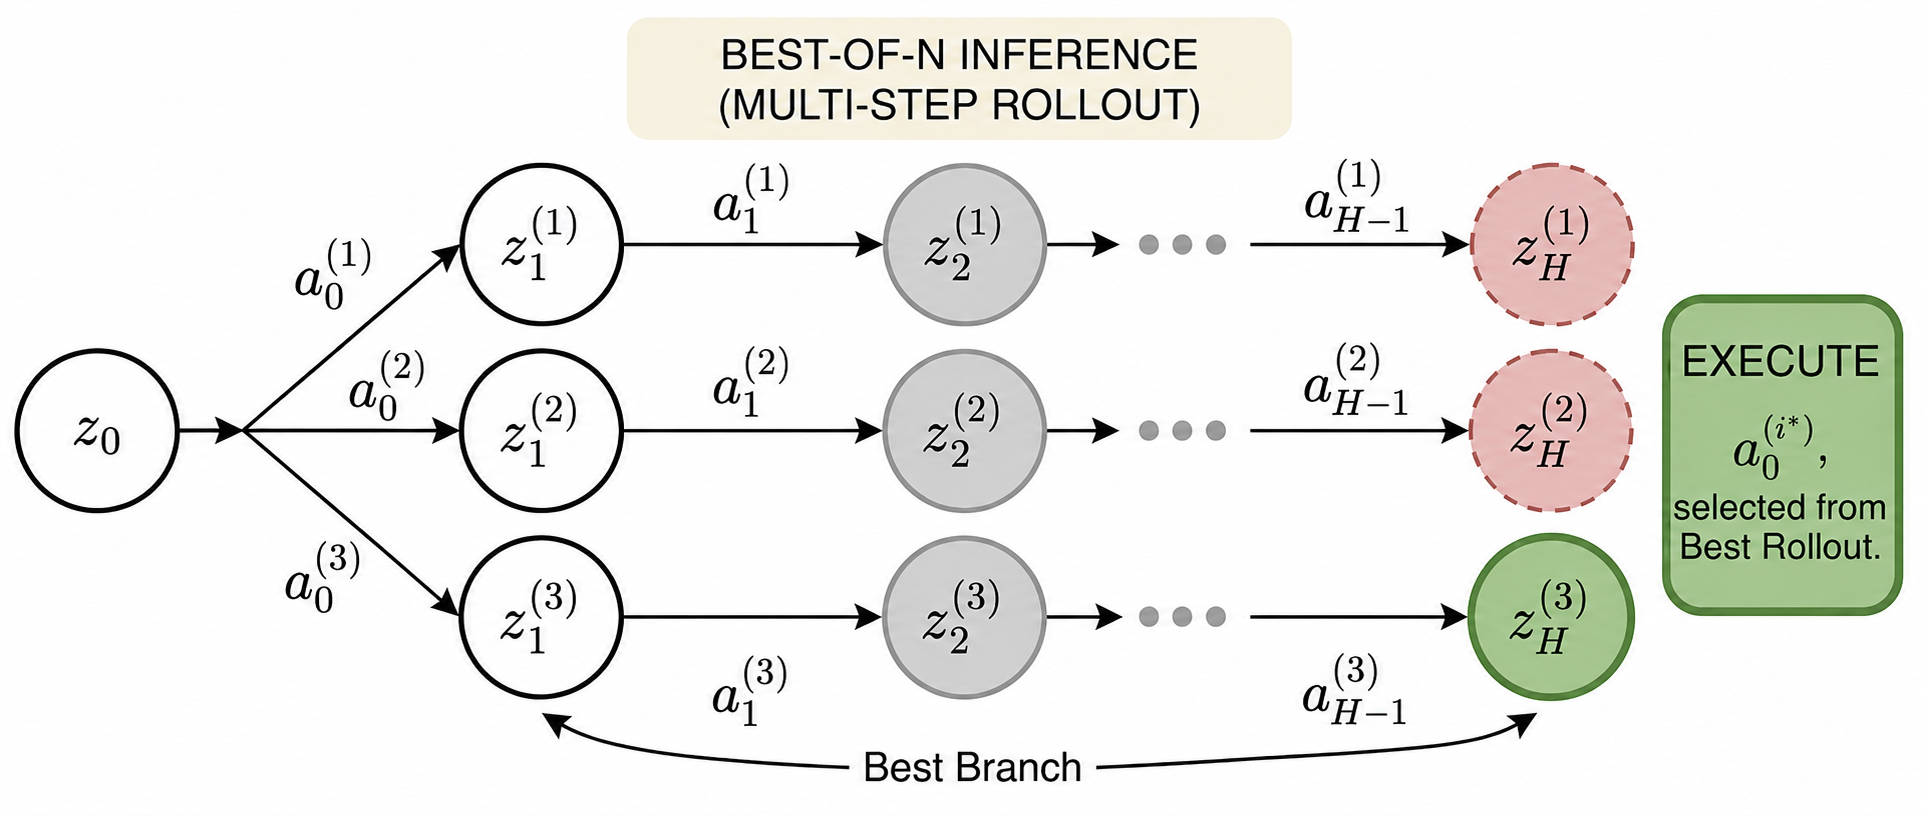
\includegraphics[width=\linewidth]{figures/bon.png}
    \caption{Illustration of Best-of-$N$ MPC at inference time. Starting from the current latent state $z_0$, the policy samples $N$ candidate first action chunks $\{a_0^{(i)}\}_{i=1}^N$. Each candidate defines a separate rollout branch, which is then propagated for $H$ steps through the world model with continuation actions re-sampled on-policy at each predicted latent state. This produces $N$ imagined trajectories with terminal latents $\{z_H^{(i)}\}_{i=1}^N$. Each rollout is scored using the critic-based objective $J$, and the branch with the highest score is selected. Only the \emph{first} action chunk $a_0^{(i^\star)}$ from the best-scoring branch is executed in the real environment.}
    \label{fig:mpc-bon}
\end{figure}

The horizon and scoring-function sweep is reported in
\S\ref{sec:exp-mpc-frozen} (Table~\ref{tab:mpc-bon}). It tests whether
additional model lookahead improves ranking or instead makes the critic
score less reliable because of predictor drift.

\begin{algorithm}[h]
\caption{Best-of-$N$ MPC inference.}
\label{alg:mpc-bon}
\begin{algorithmic}[1]
\Require current latent $z_t$, BC-flow actor $\pi_\theta$, critic $Q_\phi$, world model $f_\psi$, hyperparameters $N$, $H$, scoring $J$.
\State Tile $z_t$ to a batch $z_{\text{batch}} \in \mathbb{R}^{N \times d_z}$.
\State Sample $\{x_0^{(i)}\} \sim \mathcal{N}(0, I_{25})$ and set $a_0^{(i)} \leftarrow \Phi_\theta(z_{\text{batch}}, x_0^{(i)})$.
\State Roll each candidate forward $H$ steps through $f_\psi$ with on-policy continuation re-sampling.
\State Compute score $s_t^{(i)}$ for each candidate using $J$.
\State \Return $a_0^{(i^\star)}$ with $i^\star = \arg\max_i s_t^{(i)}$.
\end{algorithmic}
\end{algorithm}

% ---------------------------------------------------------------------
\section{Gradient-Based Value Guided Planning}
\label{sec:mpc-grad}

Best-of-$N$ MPC is fundamentally limited by the support of the
proposal distribution: it can only select actions that are already
likely under the policy. Since the world model is differentiable, we
can go beyond this limitation by directly optimising the selected
action using gradients through the model.

\paragraph{Update rule.}
Starting from the BoN winner, we run $K$ raw gradient ascent steps,
\begin{equation}
    a_0 \;\leftarrow\; \mathrm{clip}\!\Big(a_0 + \eta\,\nabla_{a_0} J(a_0;\,z_t),\;-1,\;1\Big),
    \qquad k = 1, \dots, K,
    \label{eq:mpc-grad}
\end{equation}
with step size $\eta = 0.01$ and $K=5$. This procedure, referred to
as Grad-MPC, can be seen as replacing discrete sampling in MPC with
continuous optimisation through backpropagation across the world
model rollout. It is closely related to TD-MPC-style refinement \cite{hansen2022temporaldifferencelearningmodel}, but
differs in that the optimisation is performed entirely at inference
time and is applied only to the first action chunk.

\paragraph{Gradient-step sensitivity.}
The number of gradient steps controls the trade-off between refinement
and critic extrapolation. Too few steps provide little movement beyond
the sampled proposal, while too many steps may push actions into regions
where the critic has limited support. The sweep over refinement settings
is reported in \S\ref{sec:exp-mpc-frozen} (Table~\ref{tab:mpc-grad}).

% ---------------------------------------------------------------------
\section{Flow-Matching $Q$-Guided Planning}
\label{sec:mpc-fmq}

Grad-MPC relies on iterative optimisation, which introduces both
computational overhead and sensitivity to step size. Flow Map
$Q$-Guidance (FMQ) \cite{ziakas2026aligningflowmappolicies} replaces this iterative process with a
closed-form update derived from a trust-region approximation of the
critic.

\paragraph{Trust-region objective.}
Let $\pi^{\mathrm{ref}}(\cdot \mid z)$ be a reference flow-map
policy producing actions $a_1 = a_r + (1-r)\,u^{\mathrm{ref}}_{r,1}(a_r \mid z)$
through the two-time average velocity $u^{\mathrm{ref}}_{r,1}$.
We seek a perturbation of this velocity field that improves the
critic while remaining close to the original policy:
\begin{equation}
    \max_{u_{r,1}}\; Q_\phi\!\big(z,\, a_r + (1-r)\, u_{r,1}(a_r \mid z)\big)
    \qquad\text{s.t.}\qquad
    \big\|u_{r,1} - u^{\mathrm{ref}}_{r,1}\big\|_2 \;\le\; \eta.
    \label{eq:mpc-fmq-objective}
\end{equation}

\paragraph{Closed-form solution.}
The solution to this constrained optimisation problem is given by:
\begin{equation}
    \boxed{\;u^{\,*}_{r,1}(a_r \mid z) \;=\; u^{\mathrm{ref}}_{r,1}(a_r \mid z) \;+\; \eta\,\frac{\nabla_a Q_\phi(z, a_1)}{\big\|\nabla_a Q_\phi(z, a_1)\big\|_2}\;.}
    \label{eq:mpc-fmq-target}
\end{equation}
This update has a clear interpretation: it preserves the original
policy direction and adds a fixed-magnitude step in the direction
that most increases the critic.

\paragraph{Inference-time FMQ.}
FMQ replaces the iterative refinement loop of Grad-MPC with a single
application of this update. Otherwise, the proposal sampling,
rollout, and scoring procedure are identical.
Algorithm~\ref{alg:mpc-fmq} shows the complete FMQ inference procedure.
Each policy proposal is refined once using a normalised critic gradient
through the world-model rollout, then the refined proposals are scored
and the best first action chunk is executed.

\begin{algorithm}[h]
\caption{Inference-time FMQ planning.}
\label{alg:mpc-fmq}
\begin{algorithmic}[1]
\Require current latent $z_t$, actor $\pi_\theta$, critic $Q_\phi$, world model $f_\psi$, scoring rule $J$, hyperparameters $N$, $H$, $\eta$.
\State Sample first-action proposals $\{a_0^{(i)}\}_{i=1}^N \sim \pi_\theta(\cdot \mid z_t)$.
\For{$i = 1, \dots, N$}
    \State Roll out $a_0^{(i)}$ for $H$ world-model steps, sampling continuation actions from $\pi_\theta$ with fixed noises.
    \State $g_i \leftarrow \nabla_{a_0^{(i)}} J(\tau_i)$ by backpropagating through the rollout $\tau_i$.
    \State $\tilde a_0^{(i)} \leftarrow \mathrm{clip}\big(a_0^{(i)} + \eta\, g_i / (\|g_i\|_2+\varepsilon),\;-1,\;1\big)$.
\EndFor
\For{$i = 1, \dots, N$}
    \State Roll out $\tilde a_0^{(i)}$ from $z_t$ for $H$ world-model steps with fresh continuation actions from $\pi_\theta$.
    \State $s_i \leftarrow J(\tilde\tau_i)$ for the resulting trajectory $\tilde\tau_i$.
\EndFor
\State \Return $\tilde a_0^{(i^\star)}$ with $i^\star = \arg\max_i s_i$.
\end{algorithmic}
\end{algorithm}

\paragraph{Sensitivity on the base critic.}
FMQ relies on the critic providing a locally meaningful gradient
direction. Since the critic is trained only on offline data generated by
the behaviour policy, large FMQ updates can move actions outside its
support. The trust-region sweep is reported in \S\ref{sec:exp-fmq-base}
(Table~\ref{tab:mpc-fmq-basepolicy}).

\paragraph{FMQ as a training signal.}
FMQ can also be used to generate improved supervision targets.
In the training pipeline of Chapter~\ref{chap:mpc-distillation},
FMQ is used to select action labels, which are then used to train the
actor via standard behavioural cloning in latent space.

% ---------------------------------------------------------------------
\section{Summary}

This chapter defined planners that keep the world model in a
short-horizon proposal role and delegate final action ranking to an
offline-trained critic. Best-of-$N$ search, gradient refinement, and FMQ
all share this proposal-and-score structure but differ in how candidate
actions are produced or refined. The next chapter uses the same planners
to generate training targets and synthetic transition data, rather than
using them only at inference time.

\chapter{World Model as Data Generator}
\label{chap:mpc-distillation}

\section{Motivation}
\label{sec:mpcd-motivation}

Chapter~\ref{chap:wm-planner} defined planners that use the world model
only at inference time. This keeps model use local and critic-guided, but
it also means that the final policy still depends on test-time search.
This raises a natural question: can the behaviour of the planner be
\emph{absorbed into the policy itself}, so that the final agent
executes at the same level without requiring any online search,
simulation, or test-time optimisation?
Instead of treating the world model as an external decision-time module,
we use it to generate supervision during training, transferring MPC
improvements into the actor so that planning becomes implicit in the
policy parameters.

We explore three progressively more integrated formulations. The
first is a static relabel-and-train pipeline
(\S\ref{sec:mpcd-offline}), where MPC is run once to generate a fixed
dataset of improved actions. The second is an interleaved procedure
(\S\ref{sec:mpcd-interleaved}), where MPC labels and policy updates
are continuously refreshed as training proceeds. The third is a full
online phase inside the world model
(\S\ref{sec:mpcd-online-wm}), where both MPC-generated actions and
world-model-imagined transitions are injected into the replay buffer,
creating generated transition data for continued training.
Across these variants, the central design question is where WM-derived
information enters learning: only as fixed labels, as periodically
updated supervision, or as full synthetic interaction data.

% ---------------------------------------------------------------------
\section{Offline Policy Learning from MPC-Generated Actions}
\label{sec:mpcd-offline}

We begin with the simplest way of converting inference-time gains into
training data: run MPC once over the offline dataset, then train the
policy to imitate the resulting actions.

\paragraph{Phase A --- relabel.}
For every latent state $z \in \mathcal{Z}_{\text{off}}$, we compute a
corresponding improved action chunk $\mathbf{a}^{\text{MPC}}(z)$ by
running Grad-MPC with parameters $N = 32$, $H = 2$, $K = 5$,
$\eta = 0.01$, and Q-term scoring, using the fully trained actor,
critic, and world model.
This produces a fixed relabelled dataset in which each state is paired
with an action that is locally improved according to the planner.

\paragraph{Phase B --- train.}
The BC-flow actor is then trained on these relabelled pairs
$(z, \mathbf{a}^{\text{MPC}})$ using the standard flow-matching loss
from Eq.~\eqref{eq:bc-flow-bg}. During this phase, both the critic
and the original network heads are frozen; only the actor is
updated. Training uses AdamW with learning rate $10^{-4}$, weight
decay $10^{-4}$, batch size $256$, for $10^5$ gradient steps.

\paragraph{Phase C --- evaluate.}
After training, the policy can be evaluated directly, or
used again as the proposal distribution inside MPC (BoN, Grad-MPC, or
FMQ), without requiring any additional training.

\paragraph{Limitations of static action relabelling.}
The main limitation is that the relabelled dataset is generated from a
fixed actor and critic, and therefore reflects a single snapshot of the
optimisation process.
As training progresses, the policy shifts away from the behaviour that
generated the labels, and the frozen relabelling critic cannot improve
the scoring function that defines $\mathbf{a}^{\text{MPC}}$. The
supervision signal therefore becomes stale, limiting continued training.
The next section addresses this by making MPC relabelling part of the
training loop itself.

% ---------------------------------------------------------------------
\section{Interleaved Policy Learning from MPC-Generated Actions}
\label{sec:mpcd-interleaved}

The key limitation of static relabelling is that MPC labels are computed
only once, even though they depend on the actor that proposes actions
and the critic that scores them. A more consistent approach is therefore
to recompute labels periodically as both networks evolve.

\paragraph{Mechanism.}
We maintain a buffer $\mathcal{B}_{\text{MPC}}$ of relabelled
transitions $(z, \mathbf{a}^{\text{MPC}}(z))$. After an initial warm-up
period of $T_{\text{warm}}$ steps, this buffer is refreshed every
$T_{\text{relabel}}$ gradient updates by sampling states from the
offline dataset and recomputing their MPC actions using the current
actor and critic.
During training, each minibatch is formed by mixing real offline
samples with relabelled MPC samples. Specifically, a fraction of each
batch is replaced with entries from $\mathcal{B}_{\text{MPC}}$, and
the standard FQL update is applied to the combined batch.

\paragraph{What the critic sees.}
Importantly, the replacement affects only the state-action pairs. The
rewards and next states remain those of the original offline
transition. Thus, the critic is updated on tuples of the form
$(z, \mathbf{a}^{\text{MPC}}, r, z')$, where $r$ and $z'$ correspond
to the environment transition induced by the original action, not the
MPC action.
In practice, this mismatch is often small because MPC actions remain
close to the behaviour policy due to local refinement. However, it is
conceptually important: the critic is being trained on transitions
that did not actually occur. The fully online variant in
\S\ref{sec:mpcd-online-wm} removes this inconsistency entirely.

\paragraph{Critic update.}
We compare an actor-only variant with a critic-update variant. In the
actor-only setting, MPC labels are used only for an additional policy
loss, while the critic continues to see the original offline actions. In
the critic-update setting, MPC-labelled actions are also inserted into
critic batches. This tests whether the actor can benefit from planner
labels when the critic has never been calibrated on the same action
distribution.

\paragraph{Grad-MPC vs FMQ labels.}
The relabelling procedure can use either Grad-MPC or FMQ. Grad-MPC
produces strong improvements but can introduce noisy action updates due
to iterative optimisation. FMQ produces more stable and structured
updates by constraining refinement to a trust region.
The Grad-MPC and FMQ relabelling results are reported in
\S\ref{sec:exp-mpc-interleaved-grad}--\ref{sec:exp-fmq-distil-inf}
(Tables~\ref{tab:mpc-interleaved-grad}, \ref{tab:mpc-relabel-sweep},
and~\ref{tab:mpc-fmq-distilled}), with the full hyperparameter sweep in
Appendix~\ref{app:oo-sweeps}. The next section removes the remaining
real-transition inconsistency by generating the successor state with the
same world model used for action selection.

\begin{algorithm}[h]
\caption{Interleaved training with MPC-generated actions.}
\label{alg:mpc-interleaved}
\begin{algorithmic}[1]
\Require offline dataset $\mathcal{D}_{\text{off}}$, FQL agent $(\pi_\theta, Q_\phi)$, frozen WM $f_\psi$, hyperparameters $T_{\text{warm}}$, $T_{\text{relabel}}$, buffer size $|\mathcal{B}_{\text{MPC}}|$, mix ratio $p$, label generator $\mathcal{M} \in \{\text{Grad-MPC},\, \text{FMQ}\}$.
\State $\mathcal{B}_{\text{MPC}} \leftarrow \emptyset$.
\For{$\text{step} = 1, \dots, T_{\text{total}}$}
    \If{$\text{step} \ge T_{\text{warm}}$ \textbf{and} $\text{step} \bmod T_{\text{relabel}} = 0$}
        \State Sample $|\mathcal{B}_{\text{MPC}}|$ states from $\mathcal{D}_{\text{off}}$.
        \State For each $z$, set $\mathbf{a}^{\text{MPC}}(z) \leftarrow \mathcal{M}(z;\,\pi_\theta,\,Q_\phi,\,f_\psi)$ using Grad-MPC (\S\ref{sec:mpc-grad}) or FMQ (Alg.~\ref{alg:mpc-fmq}).
        \State $\mathcal{B}_{\text{MPC}} \leftarrow \{(z,\,\mathbf{a}^{\text{MPC}}(z))\}$; reset the actor-only optimiser state.
    \EndIf
    \State Sample minibatch $B$ from $\mathcal{D}_{\text{off}}$.
    \If{$\mathcal{B}_{\text{MPC}} \ne \emptyset$}
        \State Sample $\lfloor pB \rfloor$ pairs from $\mathcal{B}_{\text{MPC}}$ and overwrite the first $\lfloor pB \rfloor$ rows of $B$'s observations and actions.
    \EndIf
    \State Update $(\pi_\theta, Q_\phi)$ on $B$ with the standard FQL critic and actor losses.
\EndFor
\end{algorithmic}
\end{algorithm}

% ---------------------------------------------------------------------
\section{Actor Fine-Tuning with World-Model Transitions}
\label{sec:mpcd-online-wm}

All methods in this chapter so far use the world model either as a
planning tool (Chapter~\ref{chap:wm-planner}) or as a way to relabel
actions in an otherwise real-data training loop
(\S\S\ref{sec:mpcd-offline}--\ref{sec:mpcd-interleaved}). In both cases,
the replay buffer remains grounded in real environment transitions.
This section goes a step further: rather than relabelling actions, we
use the world model to \emph{generate the transitions themselves}, so
that the agent effectively performs offline-to-online reinforcement
learning entirely within the learned dynamics.
This is close to the setting of Chapter~\ref{chap:wm-env}, but with two
additional constraints: actions are selected by a critic-scored MPC
controller, and successor states are generated by the same
action-conditioned model used in the rollout. The design therefore tests
whether synthetic transitions are more useful when action selection and
successor generation are kept consistent.

\paragraph{From action relabelling to full transition synthesis.}
The interleaved method (\S\ref{sec:mpcd-interleaved}) still relies on
the latents from real transitions: it modifies the action in a stored tuple but keeps the
original successor $z'$. This creates a subtle inconsistency: the critic
is trained on tuples of the form
\[
(z,\, \mathbf{a}^{\text{MPC}},\, r,\, z'),
\]
where $z'$ corresponds to the behaviour action $\mathbf{a}$, not the
MPC action $\mathbf{a}^{\text{MPC}}$. The approach works because MPC
keeps $\mathbf{a}^{\text{MPC}}$ close to $\mathbf{a}$, but it does not
represent a true transition under the modified action.

We remove this inconsistency by constructing transitions entirely inside
the world model. Starting from a real initial latent, we use FMQ-MPC to
select an action chunk $\mathbf{a}^{\text{MPC}}$ and then execute it in
the world model:
\[
z'_\psi = f_\psi(z, \mathbf{a}^{\text{MPC}}).
\]
We assign a sparse task reward in latent space,
\[
r_\psi = \mathbb{1}\{\lVert z'_\psi - z_{\text{goal}}\rVert < \delta\},
\]
and obtain a fully self-consistent synthetic transition
\[
(z,\, \mathbf{a}^{\text{MPC}},\, r_\psi,\, z'_\psi).
\]
These transitions are added to a replay buffer seeded with offline data,
and training proceeds as in standard FQL.
The key change is that the successor state is no longer inherited from
the dataset: it is now generated by the same dynamics model that
produced the action-conditioned rollout.

\paragraph{Constraints.}
At first sight, this procedure appears to reintroduce exactly the risks
identified in Chapter~\ref{chap:wm-env}. It is therefore constrained in
two ways.
First, actions are not arbitrary model rollouts but are selected by an
offline-trained critic through MPC. This means the model is only queried
along trajectories that the critic already assigns high value under real
data, effectively restricting synthetic transitions to regions close to
the data manifold.
Second, the world model is only used over short horizons inside MPC
($H=2$), where empirical drift remains limited (\S\ref{sec:wm-drift}).
Thus, the model is never required to produce long-horizon consistency,
only locally plausible one-step transitions under curated actions.

\paragraph{Training regimes.}
We evaluate two variants that differ only in whether the critic is
updated on synthetic transitions.
In the \emph{full update} variant, the critic performs standard FQL
updates on the mixed buffer. This tests whether imagined successors can
safely enter Bellman targets.
In the \emph{frozen critic} variant, the offline-trained critic is kept
fixed throughout the online phase and only used for (i) MPC scoring and
(ii) supervision of the BC-flow actor. This removes value
bootstrapping on imagined transitions. The full comparison is reported
in \S\ref{sec:exp-mpc-online-wm}
(Table~\ref{tab:mpc-online-e2}).

\paragraph{Effect of reintroducing planning at test time.}
We also evaluate whether applying MPC on top of the trained actor still
helps. This checks whether the actor has absorbed the planner's local
improvement signal or whether test-time search remains necessary.

% ---------------------------------------------------------------------
\section{Goal-Conditioned Actor Fine-Tuning with World-Model Transitions}
\label{sec:mpcd-gc}

The single-task setting isolates the online-in-WM loop, but it is also
favourable because the agent only needs to cover one narrow goal
distribution. In the goal-conditioned setting, the policy must represent
a much larger state-goal space, so world-model-driven data collection is
more likely to reduce coverage.
This section evaluates whether the same frozen-critic online-in-WM
procedure from \S\ref{sec:mpcd-online-wm} transfers to the
five-task goal-conditioned setting.

\paragraph{Setup.}
The underlying algorithm is unchanged from
\S\ref{sec:mpcd-online-wm}: FMQ-MPC is used to select actions inside
the world model, the replay buffer is augmented with imagined
transitions, and the critic is frozen so that only the BC-flow actor
is updated.
Three modifications define the goal-conditioned version. First, the
observation is augmented to include the goal embedding:
$[z, z_{\text{goal}}]$. Second, training is performed jointly across a
set of related goal-conditioned tasks rather than a single task. Third,
rewards follow the HIQL HER-style indicator formulation used in the
offline goal-conditioned baseline.
The pure offline goal-conditioned FQL checkpoint serves as the main
reference point for evaluating whether online-in-WM training provides
additional benefit.

\paragraph{HER inside the online-in-WM loop.}
During the online phase, goals can be sampled in two ways.
The default setting uses evaluation goals directly (``eval-goals''),
meaning that the same goal distribution appears both during training
and evaluation. While effective, this introduces a mild evaluation
leakage, since the agent is repeatedly trained on the exact goals it
will later be tested on.
To address this, we also evaluate a hindsight relabelling (HER)
variant \cite{her}, where goals are sampled from achieved states in
previous trajectories. Concretely, each rollout can be relabelled by
treating a future achieved state as the goal, and training goals are
drawn from a buffer of achieved states rather than the evaluation goal
set. In the indicator-reward setting, HER only modifies the goal
argument; the underlying transitions remain unchanged.
Algorithm~\ref{alg:owm-gc} summarises the full procedure.

\begin{algorithm}[h]
\caption{Goal-conditioned online-in-WM with HER. The single-task
controller of \S\ref{sec:mpcd-online-wm} is the special case in
which the goal is fixed across the entire online phase and the HER
relabelling step is skipped.}
\label{alg:owm-gc}
\begin{algorithmic}[1]
\Require offline GC checkpoint $(\pi_\theta, Q_\phi)$, frozen WM $f_\psi$, replay buffer $\mathcal{D}_{\text{off}}$ seeded with the offline transitions, achieved-state buffer $\mathcal{G}$, goal source $\mathcal{S} \in \{\text{eval}, \text{random achieved}\}$.
\State Freeze the critic $Q_\phi$.
\For{$\text{step} = 1, \dots, T_{\text{online}}$}
    \State Sample initial latent $z_0 \sim \mathcal{D}_{\text{off}}$ and goal $g \sim \mathcal{S}$ (or $g \sim \mathcal{G}$ for HER).
    \State Roll out: at each WM step $h$, $\mathbf{a}_h \leftarrow \text{FMQ-MPC}(z_h \oplus g)$ and $z_{h+1} \leftarrow f_\psi(z_h, \mathbf{a}_h)$.
    \State Compute reward $r_h = r_h^{\text{HIQL}}(z_{h+1}, g)$.
    \State Append $(z_h \oplus g,\, \mathbf{a}_h,\, r_h,\, z_{h+1} \oplus g)$ to $\mathcal{D}_{\text{off}}$ and store $z_{h+1}$ in $\mathcal{G}$.
    \State Sample minibatch from $\mathcal{D}_{\text{off}}$, take an actor-only gradient step with $Q_\phi$ frozen.
\EndFor
\end{algorithmic}
\end{algorithm}

The main limiting factor appears to be a combination of reduced
coverage and distributional drift. First, the FMQ-MPC controller
induces a narrow visitation distribution inside the world model, which
progressively biases the online buffer away from the broader
state-action coverage present in the offline data. Second, the
goal-conditioned observation space effectively increases dimensionality
relative to the single-task case, meaning that a fixed number of online
steps explores a smaller fraction of the relevant space.

A useful consistency check arises when comparing with the single-task
setting. There, critic updates on imagined transitions are a risky
design choice because the offline and generated data use different
reward scales. In the goal-conditioned setting, both offline and online
data share the same HIQL-style indicator reward convention, so the same
ablation tests whether critic updates remain fragile once the reward
scale is aligned. The corresponding results are reported in
\S\ref{sec:exp-mpc-online-wm-gc} (Table~\ref{tab:mpc-online-e3}).

\section{Static Dataset Generation with World Model}
\label{sec:mpcd-dataset-gen}

The online-in-WM method of \S\ref{sec:mpcd-online-wm} uses the world
model continuously during training: at every step it generates one MPC
transition, appends it to the replay buffer, and immediately updates
the policy. A natural alternative is to remove this coupling entirely
and use the world model only once, as a static generator of a dataset
that is then used for standard offline training.
This section evaluates whether such a decoupled use of the world model
can reproduce the benefits of online-in-WM training without requiring
any further interaction with the model during learning.

\paragraph{Experimental design.}
We construct two synthetic datasets using the frozen GC checkpoint from
\S\ref{sec:mpcd-gc}, each consisting of full trajectories:

\begin{itemize}
    \item \emph{FMQ rollout}: trajectories are generated by running
    FMQ-MPC inside the world model. At each step, FMQ selects the
    action, and the world model produces the successor state. The goal
    is used only for action selection and is not stored in the dataset.

    \item \emph{BoN rollout}: identical, but without FMQ refinement.
    Actions are taken directly from the best-of-$N$ candidate set
    produced by the BC-flow actor.
\end{itemize}

Both datasets are matched in size and episode structure to the original
offline play dataset (maximum horizon 40 or goal completion). As a
control, we also evaluate the original play dataset under the same HER
goal relabelling procedure, ensuring that all datasets are processed
with identical goal construction at training time.

\paragraph{Evaluation question.}
This experiment tests whether world-model-generated data remains useful
when data generation is decoupled from the learner. In online-in-WM
training, the current actor is repeatedly updated on the same type of
planner-improved actions it helps generate. In the static setting, a
fresh learner receives a fixed corpus generated by another policy and
critic. The comparison is reported in \S\ref{sec:exp-wm-dataset-gen}
(Table~\ref{tab:wm-dataset-gen}).
% ---------------------------------------------------------------------
\section{Summary}
\label{sec:mpcd-discussion}

This chapter defined three ways of turning planner improvements into
training signal: fixed MPC labels, periodically refreshed MPC labels,
and full online fine-tuning inside the world model. The key distinction
is how tightly generated data remains coupled to the current actor and
critic. The detailed results are reported in
\S\S\ref{sec:exp-mpc-interleaved-grad}--\ref{sec:exp-wm-dataset-gen} and
summarised in \S\ref{sec:exp-headline}.

\chapter{World Model for Subgoal Planning}
\label{chap:wm-as-subgoal}
\label{chap:latent-subgoal-planning}

\section{Motivation}
\label{sec:lsp-motivation}

The previous chapters showed that a frozen world model is most useful
when it proposes short-horizon futures that are scored by a value
function trained on real data. This chapter asks whether the same
proposal-and-score pattern extends from action-level planning to
hierarchical decision making.
In standard hierarchical offline RL, the high-level policy is typically learned by behaviour cloning. It proposes subgoals that already appear in the dataset, and the low-level policy is trained to reach them. This works well but is inherently conservative. If a useful subgoal was never explicitly observed in the dataset, the high level cannot propose it, even if it would be reachable under the dynamics learned by the world model.
We therefore explore whether the world model and offline value function can be used to search over subgoals rather than merely evaluate actions. The key idea is to treat subgoals as latent states in the same space as the world model, and to rank them using long-horizon value estimates obtained by rolling out the low-level policy inside the world model. In other words, we lift the same MPC-style mechanism from action space to subgoal space.

To study this, we introduce \textbf{Latent Subgoal Planning (LSP)}. The high-level policy proposes candidate subgoals directly in the learned latent space, the world model evaluates them by simulating low-level rollouts toward each candidate, and an offline-trained value function scores the resulting outcomes. This mirrors the structure of the previous chapters, but moves the search problem one level up the hierarchy.
We adopt the hierarchical framework of HIQL-style offline goal-conditioned RL, but replace the original discrete or dataset-constrained subgoal distribution with a continuous flow-matching policy over latent subgoals and actions (see \S\ref{sec:lsp-flow}). Importantly, the core HIQL structure remains unchanged: a high-level policy proposes subgoals every $k=10$ steps, and a low-level policy executes primitive actions conditioned on those subgoals. The modification is not in the hierarchy itself, but in how the high-level proposals are generated and evaluated.
Phase~1 follows standard offline goal-conditioned HIQL training with no world model involvement. Phase~2 then attempts to improve the high-level policy using world-model rollouts and value-function scoring in the same proposal-and-score spirit as Chapter~\ref{chap:wm-planner}. The evaluation in \S\ref{sec:exp-wm-as-subgoal} tests whether this action-level pattern transfers to hierarchical subgoal spaces.

% =====================================================================
\section{Latent Subgoal Planning Architecture}
\label{sec:lsp-architecture}

The system consists of three components operating in the learned latent space $\mathcal{Z} = \mathbb{R}^{d_z}$: a value function, a high-level policy, and a low-level policy.

\paragraph{Value function.}
We use an action-free goal-conditioned value function $V(z, g)$ trained with implicit Q-learning (IQL) via expectile regression (\S\ref{sec:iql}). It is trained entirely on offline data and is never updated with world-model-generated transitions. It estimates long-horizon return from state $z$ toward goal $g$.

\paragraph{High-level policy.}
The high-level policy $\pi^{\mathrm{HL}}$ proposes a subgoal latent $w$ conditioned on the current state and task goal:
\begin{equation}
w \;\sim\; \pi^{\mathrm{HL}}(\,\cdot\mid z,\,g).
\end{equation}
Unlike standard HIQL, where subgoals are implicitly constrained to match dataset behaviour, here $w$ is a continuous latent in the same space as $z$ and $g$. This makes it directly compatible with the world model, which can evaluate candidate subgoals by simulating trajectories toward them.

\paragraph{Low-level policy.}
The low-level policy $\pi^{\mathrm{LL}}$ maps the current latent and subgoal to primitive actions:
\begin{equation}
a \;\sim\; \pi^{\mathrm{LL}}(\,\cdot\mid z,\,w).
\end{equation}
The high-level policy replans every $k=10$ steps, following the standard horizon choice used in HIQL-style hierarchical control. Between replanning steps, the low-level policy executes actions conditioned on a fixed subgoal.

\subsection{Flow-Matching High- and Low-Level Policies}
\label{sec:lsp-flow}

Both policies are parameterised as flow-matching models, following the same construction used in Chapter~\ref{chap:wm-planner}. We do not restate the full formulation here and refer instead to \S\ref{sec:lsp-architecture} and the flow policy background (\S\ref{sec:fql-bg}).
The key idea is that instead of modelling a unimodal Gaussian over subgoals or actions, the policy learns a transport map from Gaussian noise to the empirical behaviour distribution. This is particularly important in high-dimensional latent spaces such as $\mathbb{R}^{d_z}$, where behaviour is highly multi-modal and concentrated on narrow manifolds.

Training follows the standard flow-matching behaviour cloning objective. Given a target sample $x_1$ (either a subgoal $w$ or an action $a$), we interpolate between Gaussian noise $x_0 \sim \mathcal{N}(0, I)$ and the target:
\begin{equation}
x_t = (1-t)\,x_0 + t\,x_1, \qquad t \sim \mathrm{Unif}[0,1],
\end{equation}
and train a velocity field to predict the displacement:
\begin{equation}
\mathcal{L}_{\mathrm{BC}}
= \mathbb{E}\!\left[
\|u_\theta(\mathrm{cond},\,x_t,\,t) - (x_1 - x_0)\|_2^2
\right].
\label{eq:lsp-bc}
\end{equation}
At inference time, samples are generated by integrating the learned velocity field using $S$ Euler steps. In Phase~2, these generated samples are further reweighted using advantage signals derived from the value function, following the same HIQL-style idea of advantage-weighted regression.

\subsection{Offline Hierarchical Training}
\label{sec:lsp-phase1}

Phase~1 trains the full hierarchical system purely offline, without any world model interaction. The value function is trained using expectile regression (\S\ref{sec:iql}), and both policies are trained using advantage-weighted flow-matching.

For each transition, an advantage estimate is computed from the value function and used to weight the flow-BC objective:
\begin{equation}
w_t = \min\!\bigl(\exp(\alpha\,\hat{A}_t),\,100\bigr),
\qquad
\hat{A}_t = \tfrac{1}{2}\sum_{i=1}^{2}
\bigl[
V_{\phi_i}(z_{t+1}, g_{\mathrm{sub}}) - V_{\phi_i}(z_t, g_{\mathrm{sub}})
\bigr].
\end{equation}
The clipping at $100$ prevents a small number of high-advantage transitions from dominating optimisation. The resulting Phase~1 policy provides the offline hierarchical baseline used by the Phase~2 world-model updates; its performance is reported in \S\ref{sec:exp-lsp-phase1} (Table~\ref{tab:lsp-phase1}).

% =====================================================================
\section{Using World Model to Improve High-Level Policies}
\label{sec:lsp-phase2}

After Phase-1, the high-level policy has learned a strong but dataset-limited mapping from $(z,g)$ to subgoals. It proposes latents that are consistent with the dataset distribution, but cannot reliably extrapolate beyond it. Phase-2 investigates whether the world model can be used as a proposal evaluator that reshapes this distribution using imagined rollouts, without ever changing the low-level policy or the value function.
Across all experiments, the value function $V$ and the low-level policy $\pi^{\mathrm{LL}}$ are frozen at their Phase-1 parameters. Only the high-level policy $\pi^{\mathrm{HL}}$ is updated. The world model is used to evaluate a candidate subgoal $w$ by first executing the low-level controller inside the model for $k$ steps starting from the current latent $z$, as illustrated in Figure~\ref{fig:lsp-subgoal-grounding}. Concretely, the low-level policy is unrolled conditionally on $w$, and the resulting latent after $k$ steps is
\begin{equation}
z_{\mathrm{ach}} = z_k,\quad
z_{h+1} = f_\psi\!\bigl(z_h, a_h\bigr),\quad
a_h \sim \pi^{\mathrm{LL}}(\cdot \mid z_h, w),\quad
z_0 = z,\quad h=0,\dots,k-1.
\label{eq:lsp-roll}
\end{equation}
The subgoal is then evaluated by how much downstream value it produces under the frozen critic, i.e. $V(z_{\mathrm{ach}}, g)$.

\begin{figure}[t]
    \centering
    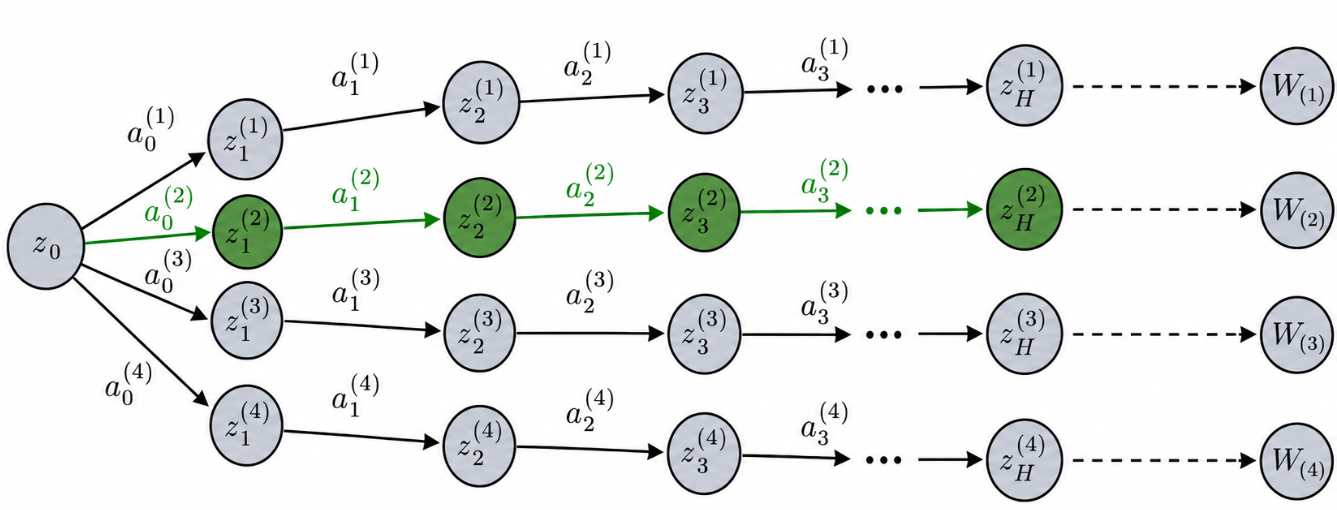
\includegraphics[width=\linewidth]{figures/subgoal_grounding.png}
    \caption{World-model-based evaluation of candidate high-level subgoals in Phase-2 of Latent Subgoal Planning. Starting from the current latent state $z_0$, the high-level policy proposes multiple candidate subgoals. For each candidate, the frozen low-level policy is rolled out for $H$ steps inside the world model, producing an imagined latent trajectory and a terminal latent $z_H^{(i)}$. Each terminal latent is then scored using the frozen value function $V$, yielding a weight or ranking for the corresponding candidate subgoal. The highest-scoring rollout indicates which subgoal is predicted to produce the greatest downstream value relative to the ultimate goal.}
    \label{fig:lsp-subgoal-grounding}
\end{figure}

The core question in all subsequent methods is whether we can use this imagined closed-loop rollout to reshape the distribution of high-level subgoals without breaking the alignment between the high- and low-level policies learned in Phase-1.

\subsection{AWR with Dataset Subgoal Targets}
\label{sec:lsp-awr-data}

The first and most direct idea is to keep the Phase-1 subgoal support fixed and simply reweight it using world-model rollouts. For each training state $z$, we sample a small set of candidate subgoals $\{w_n\}_{n=1}^N$ from the original dataset subgoal distribution used in Phase-1. Each candidate is evaluated by rolling the frozen low-level policy for $k$ steps inside the world model as in Eq.~\eqref{eq:lsp-roll}, producing $z_{\mathrm{ach},n}$.

We define an advantage relative to the current state:
\begin{equation}
J_n = V(z_{\mathrm{ach},n},\,g) - V(z,\,g),
\end{equation}
which measures whether attempting to reach $w_k$ improves predicted long-term return compared to staying at $z$. These advantages are normalised within the batch and converted into AWR weights $w_n = \min(\exp(\alpha J_n), 100)$. The high-level policy is then updated by a weighted flow-BC objective toward the dataset subgoals.

\paragraph{Distributional sharpness.}
Although this procedure is locally well-defined, it introduces a tension between the Phase-1 subgoal distribution and the broader dataset support. Phase-1 has already concentrated probability mass on a relatively narrow set of subgoals that are consistently useful under the frozen low-level policy. In contrast, the dataset distribution includes many subgoals that are valid transitions but not necessarily optimal intermediate targets.
Even with AWR weighting, every batch still contains non-zero probability mass on suboptimal subgoals. Over many updates, this can broaden the high-level flow: probability mass is pulled away from the sharp Phase-1 modes toward the wider dataset support. Increasing $\alpha$ reduces this effect but weakens the learning signal, while decreasing $\alpha$ accelerates the drift.

\subsection{AWR with On-Policy Subgoal Targets}
\label{sec:lsp-awr-self}

A natural response is to eliminate the mismatch between the dataset subgoal distribution and the current policy by sampling subgoals directly from $\pi^{\mathrm{HL}}(\cdot \mid z,g)$. This ensures that all candidates lie within the current support of the high-level policy, avoiding the broadening pressure observed above.
Each candidate subgoal $w_n \sim \pi^{\mathrm{HL}}(\cdot \mid z,g)$ is evaluated using the same world-model rollout procedure in Eq.~\eqref{eq:lsp-roll}, and scored by $V(z_{\mathrm{ach},n}, g)$. These scores are again converted into AWR weights and used to update the flow policy.

\paragraph{Value miscalibration risk.}
This variant exposes a different failure mode: the frozen value function $V(z,g)$ is not trained to evaluate arbitrary latent subgoals $w$, but only dataset-induced states. In particular, it assigns high value to latents that are close to the goal $g$, even if they are not actually reachable from $z$ within $k$ low-level steps.
As training progresses, the high-level policy exploits this bias by shifting probability mass toward subgoals $w \approx g$. However, when these subgoals are executed through the frozen low-level policy inside the world model, the resulting $z_{\mathrm{ach}}$ remains far from $g$, leading to low realised value $V(z_{\mathrm{ach}}, g)$. This creates a systematic disconnect between the training signal $V(w,g)$ and the true outcome of executing $w$ via the low-level controller, resulting in instability rather than improvement.

\subsection{AWR with Achieved Latent States}
\label{sec:lsp-hrf}

To remove the mismatch between proposed subgoals and executed outcomes, we replace the training target with the \emph{achieved state} of the rollout. Instead of regressing the high-level policy toward the proposed subgoal $w$, we regress it toward the actually reached latent $z_{\mathrm{ach}}$ obtained after executing $\pi^{\mathrm{LL}}$ in the world model for $k$ steps.

The resulting objective is:
\begin{equation}
\mathcal{L}_{\mathrm{HRF}} = \mathbb{E}\!\left[
w_n\cdot\mathcal{L}_{\mathrm{BC}}^{\mathrm{per\text{-}sample}}
\!\bigl(\pi^{\mathrm{HL}},\,z_{\mathrm{ach},n}\bigr)\right],
\quad
w_n = \min\!\bigl(\exp(\alpha\cdot\hat J_n),\,100\bigr),
\quad
J_n = V(z_{\mathrm{ach},n},\,g) - V(z,\,g).
\end{equation}
This ensures that learning is grounded in what the low-level policy can actually achieve under the world model, rather than what the high-level policy proposes.

\paragraph{Distributional mismatch between levels.}
Despite being more consistent, this objective changes the effective training distribution of the high-level policy. In Phase-1, $\pi^{\mathrm{HL}}$ is trained to produce subgoals drawn from a dataset-aligned distribution $\mathcal{D}_w$, which is itself matched to what $\pi^{\mathrm{LL}}$ expects as conditioning input.
Under HRF, the high-level policy is instead trained toward $z_{\mathrm{ach}}$, which lies in a different region of latent space: it reflects what the frozen low-level policy can reach in $k$ steps starting from $z$, not what appears as intermediate subgoals in the dataset. Although both lie in $\mathbb{R}^{d_z}$, their distributions are not aligned.
As a result, the high-level policy gradually shifts away from $\mathcal{D}_w$. The low-level policy, which has not been updated, begins to receive subgoal inputs outside its training distribution, making execution quality increasingly fragile despite the improved internal consistency of the training signal.

\paragraph{Summary of Phase-2.}
Quantitative results for the Phase-2 updates are reported in
\S\ref{sec:exp-phase2-awr} (Table~\ref{tab:lsp-phase2-awr}) and
\S\ref{sec:exp-phase2-hrf} (Table~\ref{tab:lsp-hrf}), with further
ablations in Appendix~\ref{app:lsp-ablations}. The shared distributional
risk is analysed next.

\section{High--Low Level Policy Coupling Failure Mode}
\label{sec:lsp-barrier}

The central risk in Phase~2 is not only model error or value noise, but a structural constraint of the hierarchical decomposition itself: the high-level policy $\pi^{\mathrm{HL}}$ and low-level policy $\pi^{\mathrm{LL}}$ are co-adapted in Phase~1, and their compatibility depends on a shared implicit distribution over subgoals. Any update that changes this distribution without simultaneously re-establishing that compatibility can break the equilibrium.

The three approaches can be grouped according to how they violate this constraint. Updating with dataset subgoals (Approach 1) pushes the high-level policy toward the broader dataset marginal, away from the concentrated subgoal distribution that the low-level has learned to execute reliably. Updating with on-policy subgoals preferences (Approach 2) does not change the support as drastically, but instead shifts probability mass toward near-goal or high-value regions that are not necessarily reachable within $k$ steps under the frozen low-level controller. Hindsight reality forcing (Approach 3) goes further and replaces the target distribution entirely with achieved latents $z_{\mathrm{ach}}$, which are by construction tied to the current low-level dynamics inside the world model. In each case, the effective conditioning distribution seen by $\pi^{\mathrm{LL}}$ can drift away from the one it was trained on.

A useful diagnostic is to remove the world model from the advantage computation entirely. In this controlled ablation, WM-evaluated advantages are replaced with
$V(w_k, g) - V(z, g)$ computed directly from the frozen critic, while the dataset-subgoal AWR update is otherwise unchanged. This isolates whether the central issue is compounding model error or the mismatch between the subgoal distribution induced by Phase-2 updates and the distribution on which the hierarchical policies were jointly trained. The world model can make this mismatch explicit, but it is not the only possible source of the mismatch.

\paragraph{Jointly updating the hierarchy.}
A natural repair is to update both levels so that the low-level policy can track the evolving subgoal distribution induced by the high-level updates. We evaluate this directly by allowing $\pi^{\mathrm{LL}}$ to train under the same WM-derived supervision as $\pi^{\mathrm{HL}}$. This ablation tests whether distributional drift can be absorbed by the hierarchy itself, or whether moving both policies simply shifts the inconsistency to the value function and remaining offline anchors, which still reflect the original Phase-1 equilibrium.

The underlying risk mirrors the moving-target problem analysed in Chapter~\ref{chap:mpc-distillation}. Here, the analogue is the frozen value function and the jointly trained policies: once one part of the system shifts its effective data distribution, the others can only remain consistent by shifting as well. We therefore conjecture that successful joint optimisation would require either (i) a value function that tracks the evolving hierarchy, or (ii) a mechanism that constrains both levels to a shared, fixed subgoal distribution throughout training. We leave both directions as future work.

\section{Summary}
This chapter defined a hierarchical extension of the proposal-and-score
pattern used in action-level planning. As argued in
\S\ref{sec:lsp-barrier}, the key methodological issue is the coupling
between the high-level subgoal distribution and the low-level policy
trained to execute it. Improving the high level therefore requires
maintaining that compatibility, not only finding higher-valued candidate
subgoals.

\chapter{Evaluation}
\label{chap:experiments}

This chapter evaluates the methods developed throughout the thesis and
examines the central question motivating this work: \emph{how can a
learned world model be used to improve goal-conditioned control in
high-dimensional robotic manipulation tasks?}
The chapter proceeds from the most direct uses of the world model to the
more constrained ones. We begin by evaluating the model in isolation,
using model-predictive planning directly in latent space to establish
what can be achieved without policy learning
(\S\ref{sec:exp-cem-baseline}). We then test whether the world model can
replace the training environment for reinforcement learning
(\S\ref{sec:exp-wm-as-env}), before turning to MPC methods that keep the
model in a short-horizon proposal role. Finally, we evaluate the
hierarchical framework and compare the main approaches against the
strongest baselines across the benchmark suite.
Unless otherwise stated, all results are reported using the standard
OGBench evaluation protocol in the real MuJoCo environment. Additional
ablations and supporting experiments, including resolution studies,
TD-MPC2 comparisons, and partial world-model fine-tuning experiments,
are provided in the appendix.

% ---------------------------------------------------------------------
\section{Evaluation Setup}
\label{sec:exp-setup}

Experiments are conducted using the OGBench benchmark
\cite{ogbench_park2025}, which provides a suite of goal-conditioned
robotic manipulation tasks built on top of MuJoCo. The primary benchmark
used throughout this thesis is the
\texttt{cube-single-play} domain, consisting of five object-manipulation
tasks (\texttt{horizontal}, \texttt{vertical1},
\texttt{vertical2}, \texttt{diagonal1}, and
\texttt{diagonal2}). Observations are $224\times224$ RGB images and
actions are represented as five-step chunks of $5$-dimensional
end-effector commands.
World-model training and offline reinforcement-learning datasets are
constructed from the expert demonstrations distributed with OGBench.
For the offline-to-online experiments of
Chapters~\ref{chap:wm-env}-\ref{chap:mpc-distillation}, we additionally use the
\texttt{visual-cube-single-singletask-task1-v0} benchmark to enable
direct comparison with previously reported results
\cite{li2026reinforcementlearningactionchunking}.

The primary evaluation metric throughout this chapter is the
\emph{native OGBench success rate}. Policies are deployed in the real
MuJoCo simulator and a trial is counted as successful if the manipulated
cube finishes within $4$\,cm of the target pose. Results on the
multi-task benchmark are averaged over $50$ evaluation episodes per
task, while offline-to-online experiments use $250$ evaluation episodes
to reduce variance.

One exception is the CEM planning baseline in
\S\ref{sec:exp-cem-baseline}. Following the evaluation protocol used in
LeWM \cite{maes2026leworldmodelstableendtoendjointembedding},
we additionally report a \emph{latent-reaching} metric that measures
whether planning in latent space succeeds in reaching a target latent
state. This metric is useful for diagnosing world-model behaviour, but
it should not be interpreted as a measure of task completion and is not
used elsewhere in this chapter.

\subsection{World Model and Agent Instantiation}
\label{sec:exp-wm-instantiation}

We instantiate the latent action-conditioned world model from
Chapter~\ref{chap:foundations} using LeWM
\cite{maes2026leworldmodelstableendtoendjointembedding}. We use the
public implementation and train it on the same OGBench trajectories as
the downstream policies. The encoder $E_\xi$ is a ViT-Tiny model
\cite{dosovitskiy2021vit,touvron2021deit} that maps $224\times224$ RGB
observations to $192$-dimensional latent states. The predictor
$f_\psi$ is a Transformer that receives a short latent history and an
action chunk. Each world-model step corresponds to $h=5$ primitive
actions, so the predictor operates on $25$-dimensional action chunks
$c=(a_0,\ldots,a_4)\in\mathbb{R}^{25}$. The isotropy term in
Eq.~\eqref{eq:lewm-total-clean} is implemented as the Spectral Isotropy
Regulariser (SIGReg).

Unless stated otherwise, all experiments use the action-chunked Flow
Q-Learning (FQL) agent introduced in \S\ref{sec:fql-bg}, again with
chunk length $h=5$. The main optimisation constants are fixed across
experiments: discount factor $\gamma=0.99$, target-network Polyak
coefficient $\tau=0.005$, an ensemble of two critics averaged for value
estimation, and a one-step flow distillation coefficient
$\alpha=100$. The sparse-reward threshold in \S\ref{sec:wmep-setup} is
set to $\delta=2.0$, following the latent geometry analysis in
\S\ref{sec:wm-geometry}. Other implementation constants are listed in
Appendix~\ref{app:impl}.

% ---------------------------------------------------------------------
\section{World Model Diagnostics}
\label{sec:wm-quality}

The performance of all methods developed in this thesis ultimately
depends on the quality of the learned world model. Since the world
model is used both as a latent-state encoder and as a simulator for
imagined rollouts, any prediction error directly limits the quality of
the rewards, values, and subgoals produced by downstream algorithms.
Understanding these limitations is therefore essential for interpreting
the results presented in later chapters.

This section evaluates the world model from three complementary
perspectives. First, we measure how prediction error accumulates as
the rollout horizon increases (\S\ref{sec:wm-drift}), providing an
estimate of how far into the future the model can be trusted. Second,
we examine the geometry of the latent space induced by SIGReg
(\S\ref{sec:wm-geometry}), which underpins the distance-based rewards
used throughout this thesis. Finally, we compare world models trained
on different environments to assess how these properties generalise
across tasks (\S\ref{sec:wm-quality-envs}).

% \subsection{Pre-training}
% \label{sec:wm-pretrain}
% The predictor used throughout is the
% \texttt{version\_1} checkpoint, trained for $19$ epochs on the OGBench
% cube data ($224{\times}224$ images) with the LeWM loss of
% Eq.~\eqref{eq:lewm-total-clean}; validation prediction loss settles at
% $\approx 2.5 \times 10^{-3}$ and validation SIGReg at $\approx 1.4$.

\subsection{Prediction Drift over Rollout Horizon}
\label{sec:wm-drift}

A key property of any learned dynamics model is how prediction errors
accumulate over time. Even small inaccuracies compound when predicted
states are repeatedly fed back into the model, causing imagined
trajectories to gradually diverge from reality. We quantify this
effect using \emph{latent-space drift}.

Starting from a real trajectory, a short history of latent states and
actions is provided to the predictor $f_\psi$. The model is then rolled
forward for $\Delta$ future frames, and the predicted latent state
$\hat z_{t+\Delta}$ is compared against the latent representation of
the true observation at the same timestep. Drift is measured as the
Euclidean distance

\begin{equation}
\|\hat z_{t+\Delta} - z_{t+\Delta}\|_2.
\end{equation}
Table~\ref{tab:drift} reports the average drift measured on the
\texttt{visual-cube-single} environment. We focus on this environment
because it is the only OGBench task for which the original LeWM
authors provide pretrained checkpoints, making it the foundation of
all subsequent experiments.

\begin{table}[h]
\centering
\caption{Mean latent-space prediction drift as a function of rollout
horizon. Larger values indicate greater divergence between predicted
and ground-truth latent states.}
\label{tab:drift}
\begin{tabular}{lccccc}
\toprule
Prediction horizon $\Delta$ (frames) & 1 & 5 & 10 & 25 & 50 \\
\midrule
Mean drift $\|\hat z_{t+\Delta}-z_{t+\Delta}\|_2$
& 1.77 & 3.40 & 6.10 & 11.80 & 16.54 \\
\bottomrule
\end{tabular}
\end{table}

Several observations can be made from these results. First, prediction
error grows steadily with rollout horizon, as expected for an
autoregressive dynamics model. A single world-model step corresponds
to one action chunk of five environment frames. At this horizon the
average error is only $3.4$, indicating that short-horizon predictions
remain reasonably accurate.

More importantly, these values must be interpreted relative to the
scale of the latent space itself. Across the dataset, the average
distance between two latent states is approximately $7.4$. This
provides a useful reference point: once prediction drift becomes
comparable to this value, the model's uncertainty is on the same scale
as meaningful state differences.

This transition occurs after approximately two world-model steps
($10$ frames), where the average drift reaches $6.1$. Beyond this
point, prediction error is large enough that imagined states may be
closer to modelling artefacts than to the true future dynamics. At a
horizon of $25$--$50$ frames, the accumulated error substantially
exceeds the average latent-state separation, suggesting that long
open-loop rollouts should be treated with caution.

These findings have direct implications for the algorithms introduced
later in the thesis. Methods that rely only on short-horizon
predictions, such as reward shaping or local subgoal generation, can
operate within the model's reliable regime. In contrast, approaches
that perform long imagined rollouts must account for substantial model
bias. This limitation motivates several of the design choices made in
Chapter~\ref{chap:wm-as-subgoal}, where world-model predictions are used only for
short-horizon subgoal evaluation while value estimation remains
grounded in real data.

\subsection{Latent Geometry Analysis}
\label{sec:wm-geometry}

Many of the methods introduced in later chapters use Euclidean distance
in latent space as either a reward signal or a measure of progress
towards a goal. This only makes sense if distances have a consistent
interpretation throughout the latent space. For example, if some states
naturally had very large latent norms while others had very small norms,
then the same distance threshold could correspond to very different
amounts of semantic change depending on where the agent was located.
Any reward based on latent distance would therefore require extensive
per-task tuning.

SIGReg was introduced during world-model training specifically to avoid
this issue. Rather than allowing latent representations to spread
unevenly through the embedding space, it encourages the latent
distribution to remain approximately isotropic, meaning that all
directions and regions of the space have a similar scale. In practice,
this implies that latent norms should be concentrated around a common
value rather than varying dramatically across states.

Figure~\ref{fig:latent-norms} shows the distribution of latent norms for
goal states drawn from outside the training set. The goal latent norms lie on a
similar-radius shell rather than occupying regions with very different
absolute scales. This matters because Euclidean thresholds would be hard
to interpret if some goals naturally had much larger norms than others:
distance would then be dominated by where the goal sits relative to the
origin rather than by local state similarity. Throughout this thesis we
use a fixed success threshold $\delta_d = 2.0$ in latent space, so this
plot is a sanity check that a single threshold is at least geometrically
well conditioned. The later CEM baseline tests the separate question of
whether latent proximity is sufficient for native task success.

\begin{figure}[h]
\centering
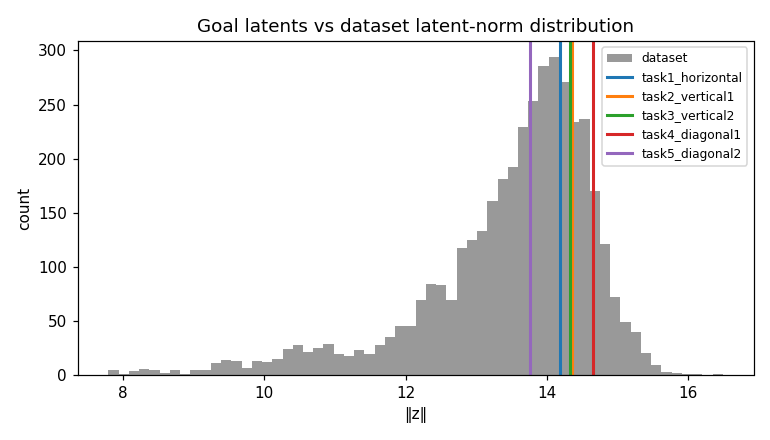
\includegraphics[width=0.55\linewidth]{figures/goal_norms_ood.png}
\caption{Distribution of latent norms for out-of-distribution goal
states. The mass is concentrated around a single radius rather than
split across widely separated norm scales. This supports using one
latent-distance threshold across goals, but does not by itself imply
that latent proximity is equivalent to task completion.}
\label{fig:latent-norms}
\end{figure}

% ---------------------------------------------------------------------
\subsection{World Model Diagnostics Across Environments}
\label{sec:wm-quality-envs}

The previous sections focused on the
\texttt{visual-cube-single-v0} environment because it is the only
OGBench task for which pretrained LeWM weights are publicly available.
To evaluate whether the conclusions generalise beyond this setting, we
also train world models for two additional OGBench environments:

\begin{itemize}
    \item \texttt{visual-scene-play-v0}, a tabletop manipulation
    environment containing multiple objects and button-press tasks;
    \item \texttt{visual-puzzle-3x3-play-v0}, a sliding-tile puzzle in
    which progress depends on discrete button activations.
\end{itemize}

All three world models are trained using the same architecture and
training procedure: a ViT-Tiny encoder, Transformer predictor,
SIGReg regularisation, and $224\times224$ image observations. The
resulting models are then evaluated using the same diagnostics
introduced above.

\paragraph{Predictor drift.}

Table~\ref{tab:drift-multienv} reports predictor drift as a function of
rollout horizon for all three environments. Recall that drift measures
the latent-space error between a predicted future state and the
corresponding ground-truth encoded state. Smaller values therefore
indicate a more accurate dynamics model. Several trends are immediately visible.

First, the scene environment is substantially easier to model than the
cube environment. Drift remains low even at longer horizons, suggesting
that imagined rollouts remain reliable for several world-model steps.
Second, the puzzle environment is dramatically more difficult. After a
single world-model step ($\Delta=5$ frames), the average prediction
error already exceeds $8.8$, which is larger than the average distance
between many semantically distinct states in the cube environment.
Errors then continue to grow with rollout horizon.
We believe this difference is a consequence of the underlying task
dynamics. The cube and scene environments are dominated by smooth,
continuous object motion, which is well suited to latent prediction.
The puzzle environment, by contrast, contains discrete button-flip
events that abruptly change the state of the puzzle. Such transitions
are difficult for a continuous predictor to anticipate accurately,
leading to significantly larger rollout errors.

\begin{table}[h]
\centering
\caption{Predictor drift
$\|\hat{z}_{t+\Delta}-z_{t+\Delta}\|_2$
across three environments. Lower values indicate more accurate
long-horizon predictions.}
\label{tab:drift-multienv}
\begin{tabular}{lcccc}
\toprule
Environment & $\Delta=5$ & $\Delta=10$ & $\Delta=25$ & $\Delta=50$ \\
\midrule
cube-single & 3.40 & 6.10 & 11.80 & 16.54 \\
scene       & 1.23 & 2.20 & 4.92 & 7.76 \\
puzzle-3x3  & 8.88 & 13.53 & 17.01 & 19.03 \\
\bottomrule
\end{tabular}
\end{table}

Figure~\ref{fig:drift-multienv} visualises the same results. The key
observation is that rollout accuracy degrades at very different rates
across environments. This suggests that downstream planning methods
should not be expected to benefit equally from a world model even when
the architecture and training procedure are identical.

\begin{figure}[h]
\centering
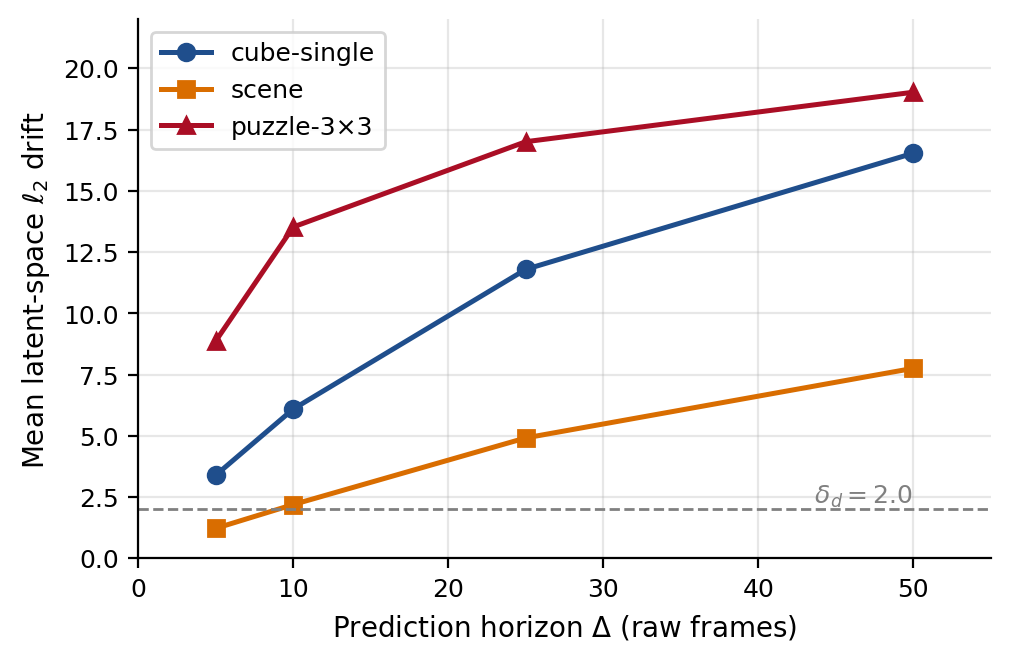
\includegraphics[width=0.68\linewidth]{figures/multi_env_predictor_drift.png}
\caption{Predictor drift as a function of rollout horizon. Lower curves
indicate more accurate imagined trajectories. The scene environment
remains predictable over substantially longer horizons than the cube or
puzzle environments.}
\label{fig:drift-multienv}
\end{figure}

\paragraph{Action conditioning.}

Predictor accuracy alone is not sufficient for planning. A planner must
also be able to influence the future state through its choice of
actions. A world model that accurately predicts the future but largely
ignores its action inputs would be unsuitable for model-based control.

To measure this property, we compare predictions generated using the
true action sequence with predictions generated using randomly shuffled
actions. If shuffling the actions causes prediction quality to
deteriorate substantially, then the predictor must be using the action
signal. Conversely, if the prediction error remains almost unchanged,
the predictor is largely insensitive to the chosen actions.

Figure~\ref{fig:action-cond} reports the resulting
action-conditioning ratio. Larger ratios indicate stronger dependence
on the action sequence and therefore greater controllability.
The cube model exhibits extremely strong action conditioning: replacing
the correct actions with shuffled actions increases prediction error by
a factor of approximately $8\times$. This indicates that the model has
learned a strong relationship between actions and future states, making
it well suited for planning.
The scene model remains action-conditioned, but much less strongly
($1.4\times$). The predictor responds to control inputs, although the
effect is relatively modest.
The puzzle model shows almost no action sensitivity
($1.1\times$). In practice, this means that imagined futures are nearly
the same regardless of which actions are supplied. Such a model may
still reconstruct the average behaviour observed in the dataset, but it
provides little useful information for selecting actions.

\begin{figure}[h]
\centering
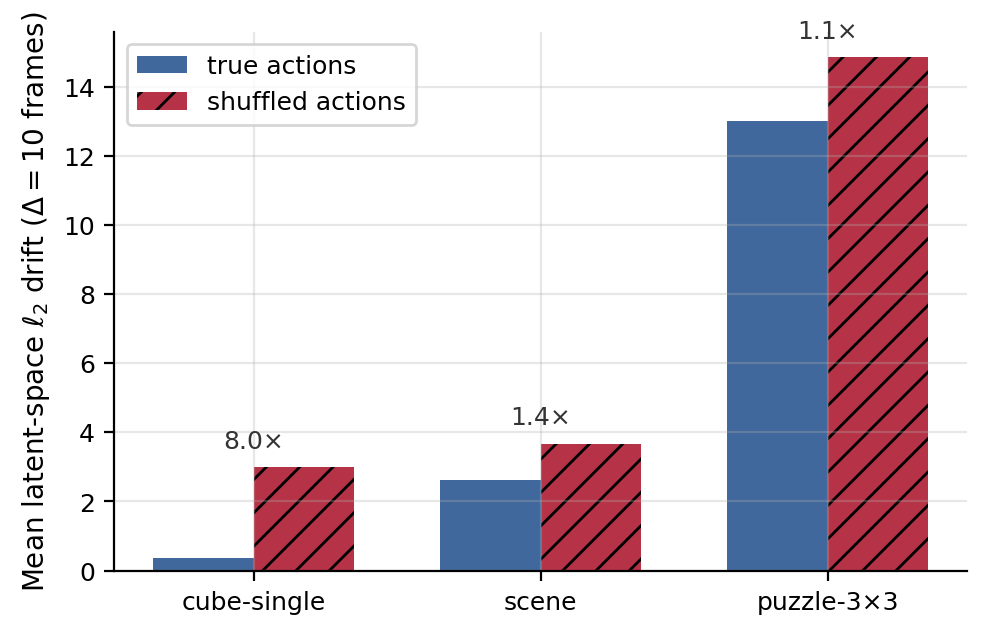
\includegraphics[width=0.65\linewidth]{figures/action_conditioning.png}
\caption{Action-conditioning diagnostic. Larger ratios indicate that
the predictor strongly depends on its action inputs, which is a
prerequisite for effective model-based planning.}
\label{fig:action-cond}
\end{figure}

\paragraph{Latent-space quality.}

Finally, we verify that the latent geometry remains well behaved across
all environments. Table~\ref{tab:norms-multienv} reports the mean and
standard deviation of latent norms for states drawn from each dataset.
The most important observation is not the exact numerical value of the
norms, but their consistency. Across all environments, latent vectors
occupy approximately the same scale and exhibit relatively small
variance. This suggests that SIGReg is successfully enforcing a
well-conditioned latent geometry regardless of task.
In addition, all goal states remain clearly separated from one another
in latent space, and no dataset state falls within the success
threshold of an incorrect goal. Consequently, the distance-based reward
functions used throughout this thesis remain meaningful without any
environment-specific recalibration.

\begin{table}[h]
\centering
\caption{Latent norm statistics across environments. Similar norm
scales indicate that SIGReg produces a consistent latent geometry even
when the underlying tasks differ substantially.}
\label{tab:norms-multienv}
\begin{tabular}{lrrl}
\toprule
Environment & Dataset mean & Dataset std & Goal mean \\
\midrule
cube-single & 13.47 & 1.26 & 14.28 \\
scene       & 13.92 & 0.70 & 13.53 \\
puzzle-3x3  & 13.80 & 0.57 & 13.97 \\
\bottomrule
\end{tabular}
\end{table}

Taken together, these diagnostics suggest that latent-space quality is
not the limiting factor for downstream performance. All three models
produce well-structured latent representations. Instead, the critical
difference lies in the interaction between prediction accuracy and
action conditioning. As we show in
\S\ref{sec:exp-generalisation}, these two properties are much more
predictive of whether model-based planning methods succeed than either
raw latent geometry or reconstruction quality alone.

% ---------------------------------------------------------------------
\section{Latent-Space Planning Baseline}
\label{sec:exp-cem-baseline}

Before evaluating learned policies, we first ask how far the frozen
world model can be pushed on its own. To answer this, we use the same
Cross-Entropy Method (CEM) \cite{Rubinstein1999} planning procedure employed in the original
LeWM work. Rather than learning a policy, CEM directly
optimises sequences of actions against the world-model dynamics,
selecting the action sequence that minimises the latent-space distance
to a target goal state.
This experiment represents the strongest possible \emph{world-model
only} baseline: planning is performed directly in the latent space used
to train the predictor, without any approximation introduced by policy
learning or value estimation.

\begin{table}[h]
\centering
\caption{CEM planning directly in the $224{\times}224$ LeWM latent
space (\texttt{terminate\_at\_goal}, $50$ episodes).
\emph{Latent-reach} is the in-distribution training-time diagnostic;
\emph{native task success} is the OGBench block-pose criterion --- the
metric every subsequent table is measured against. The contrast is
the central observation that frames the rest of this chapter.}
\label{tab:cem-baseline}
\begin{tabular}{lc}
\toprule
Setting & Value \\
\midrule
Plan / receding horizon      & 5 / 5 \\
Action block                 & 5 \\
CEM samples $\times$ iters   & $300 \times 30$ \\
CEM elite (top-$k$)          & 30 \\
\midrule
Latent-reach rate            & $72.0\%$ \\
\textbf{Native task success} & \textbf{$0.0\%$} \\
\bottomrule
\end{tabular}
\end{table}

The result (Table~\ref{tab:cem-baseline}) reveals an important limitation of the learned latent space.
While the planner successfully reaches the target latent state in
approximately $72\%$ of episodes, it fails to solve a single cube
manipulation task when evaluated in the real MuJoCo environment.
This discrepancy demonstrates that latent-space proximity and task
completion are not equivalent objectives. The world model has learned a
representation in which nearby latent states are predictive of future
observations, but reaching a target embedding does not necessarily imply
that the physical object has reached the desired configuration. In other
words, the latent geometry is useful for prediction but is not, by
itself, a sufficient control objective.
The remaining experiments therefore use latent rollouts only when their
outcomes are judged by a critic or policy trained on real task data.

% ---------------------------------------------------------------------
\section{World Model as Environment Results}
\label{sec:exp-wm-as-env}

Chapter~\ref{chap:wm-env} introduced the variants that use LeWM as a
surrogate environment for online fine-tuning. This section reports their
real-environment performance and the diagnostic comparisons needed to
interpret the failures. Across all variants tested, synthetic
world-model interaction fails to improve the offline policy.

\subsection{Offline-to-Online Reinforcement Learning inside World Model}
\label{sec:exp-oo-wm-env}

Figure~\ref{fig:wm-env-curves} shows the training curves for the
principal variants introduced in Chapter~\ref{chap:wm-env}, while
Table~\ref{tab:owm-summary} reports their final performance when
evaluated in the real MuJoCo environment.
A consistent pattern emerges across all experiments: none of the
world-model-based training procedures improve upon the offline policy
from which they start. The control row shows that the same latent
representation can support online improvement under true dynamics, so
the degradation is specific to using the predictor as the transition
model.

\begin{figure}[h]
\centering
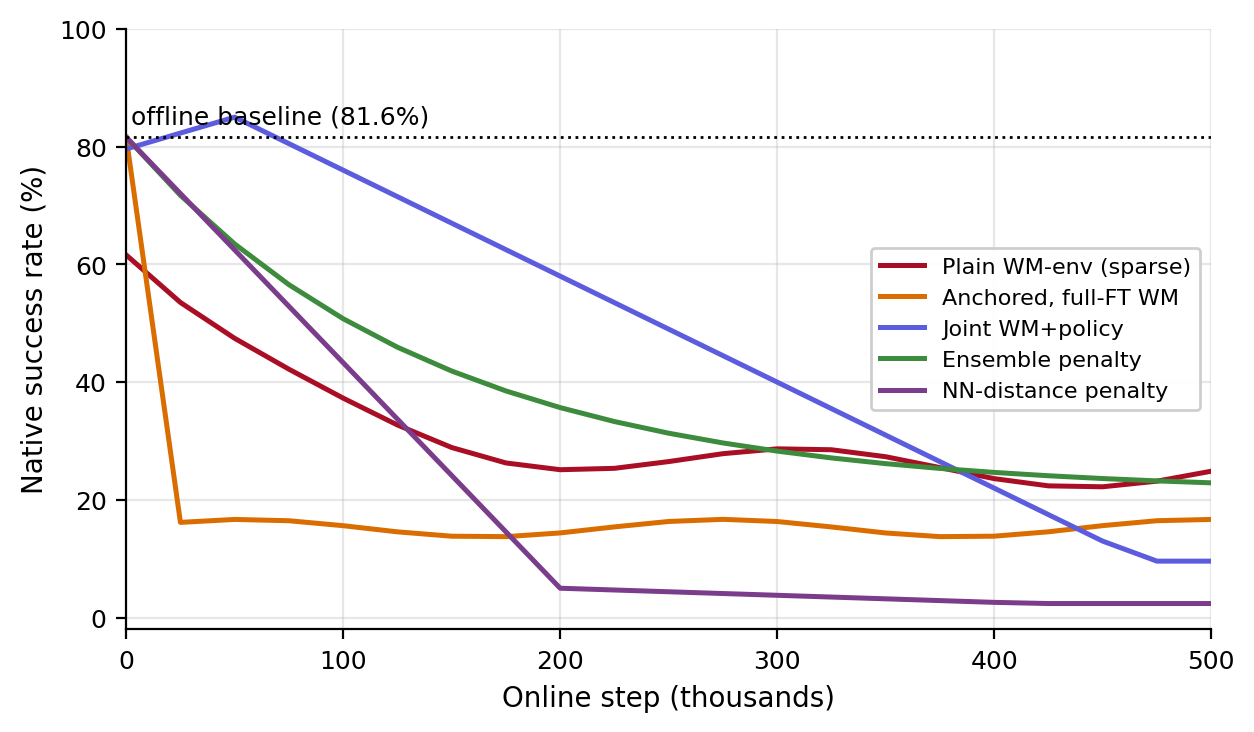
\includegraphics[width=0.85\linewidth]{figures/wm_env_training_curves.png}
\caption{Training-time success rate during world-model fine-tuning on
\texttt{visual-cube-single-singletask-task1-v0}. The horizontal dashed
line indicates the performance of the initial offline policy
($81.6\%$). All variants remain below this baseline throughout training,
demonstrating that online reinforcement learning inside the learned
world model does not translate into improved real-environment
performance.}
\label{fig:wm-env-curves}
\end{figure}

\begin{table}[h]
\centering
\caption{Final real-environment performance after the online phase for
world-model-as-environment approaches on
\texttt{visual-cube-single-singletask-task1-v0}. The main offline
starting checkpoint has $81.6\%$ success; the jointly trained policy
starts from $79.6\%$. The table reports the final online result only,
measured over $250$ evaluation episodes, except for the real-dynamics
control, which was evaluated over $50$ episodes. Multi-run settings
report mean $\pm$ standard deviation; single-run diagnostics are marked
with $1$ run.}
\label{tab:owm-summary}
\begin{tabular}{lcr}
\toprule
Variant & Runs & Final SR (\%) \\
\midrule
\multicolumn{3}{l}{\emph{Real-dynamics control}} \\
Latent observations, real dynamics & 1 & \textbf{100.0} \\
\midrule
\multicolumn{3}{l}{\emph{Direct WM interaction}} \\
Sparse reward & 3 & $24.5 \pm 5.1$ \\
Anchored, sparse reward & 3 & $17.2 \pm 4.9$ \\
Anchored, dense reward & 3 & $15.2 \pm 2.3$ \\
\midrule
\multicolumn{3}{l}{\emph{Predictor adaptation and component swap}} \\
Joint predictor--policy training & 1 & 9.6 \\
\quad Base policy + jointly trained predictor & 1 & 7.2 \\
\quad Jointly trained policy + base predictor & 1 & 30.0 \\
\midrule
\multicolumn{3}{l}{\emph{Uncertainty-penalised rewards}} \\
Ensemble uncertainty penalty & 1 & 21.2 \\
Nearest-neighbour regularisation & 1 & 2.4 \\
\bottomrule
\end{tabular}
\end{table}

The most striking observation is the contrast with the control
experiment. When the policy is trained online using the real
environment while retaining the same latent observation space,
performance improves from $81.6\%$ to perfect success. The limitation
therefore does not lie in the policy architecture or the latent
representation itself; it lies in treating the learned predictor as a
drop-in replacement for the environment.

The direct world-model interaction and anchored rows show that shortening
imagined rollouts is not enough to recover performance. Sparse
world-model interaction ends at $24.5 \pm 5.1\%$, while anchored sparse
and dense variants reach only $17.2 \pm 4.9\%$ and $15.2\%$. This
supports the interpretation from Chapter~\ref{chap:wm-env}: anchoring
can limit the most extreme predictor drift, but the replay buffer still
contains model-generated transitions whose errors enter value learning.
The uncertainty-penalised rows tell a similar story. Ensemble
disagreement improves only modestly to $21.2\%$, while nearest-neighbour
regularisation falls to $2.4\%$, consistent with the concern that
distance from the offline dataset is not the same as prediction error
and can penalise task-relevant but sparsely represented states.

\paragraph{Joint predictor--policy component swap.}
\label{sec:eval-joint}
The diagnostic rows associated with joint predictor--policy training
provide further insight. Replacing the jointly trained policy with the
original offline policy while keeping the jointly trained predictor
reduces performance to only $7.2\%$. Conversely, replacing the
jointly trained predictor with the original frozen predictor raises
performance to $30.0\%$. This points more strongly to the predictor
than to the policy as the source of the collapse: modifying the world
model during training appears to introduce errors that are subsequently
exploited by the reinforcement-learning objective. Together, these
results support the negative case developed in Chapter~\ref{chap:wm-env}:
LeWM is useful as a representation and short-horizon predictor, but not
as an unrestricted training environment.

% ---------------------------------------------------------------------

% \paragraph{Flow-DPO (CPU test only).}
% A contrastive preference update (Flow-DPO, \S\ref{sec:phase2-dpo})
% that selects the highest-scoring WM-rollout candidate as ``winner''
% and the lowest as ``loser'' was validated on CPU only. The
% WM-rollout metric $V_{\mathrm{roll}}$ fell from $-34.4$ to $-46.3$
% in $20$ steps --- the sharpest degradation of any approach tested
% --- owing to high gradient correlation between winner and loser in
% the Phase-1 flow's concentrated distribution. Flow-DPO was not run
% on the cluster.

% ---------------------------------------------------------------------
\section{World Model as Planner Results}
\label{sec:exp-mpc}

Chapter~\ref{chap:wm-planner} introduced the inference-time planners.
Here we evaluate them on the frozen offline policy. The pattern is
simple: short-horizon planning improves action selection, while longer
rollouts lose reliability as world-model error accumulates.

\subsection{Scoring Functions}
\label{sec:exp-scoring}

We use the three scoring rules defined in
Chapter~\ref{chap:wm-planner}: terminal critic scoring (Q-term),
trajectory-wide critic scoring (Q-all), and latent-distance shaping plus
terminal critic scoring (Dense+Q). Unless otherwise stated we use
Q-term. Q-all becomes useful later, after the critic has been trained on
planner-shaped actions.

\subsection{Inference-Time MPC on a Frozen Policy}
\label{sec:exp-mpc-frozen}

We first evaluate planning without any parameter updates. Starting from
the $81.6\%$ offline checkpoint, BoN-MPC samples $N=32$ action chunks
and ranks their short rollouts. Grad-MPC then adds five gradient-ascent
steps through the differentiable world model. Any improvement therefore
comes from test-time computation alone.

\begin{table}[h]
\centering
\caption{Best-of-$N$ MPC applied to a frozen offline policy.
Performance is measured in the real environment over 250 evaluation
episodes. The offline policy achieves 81.6\% success without planning.}
\label{tab:mpc-bon}
\begin{tabular}{l c l r}
\toprule
Method & Horizon $H$ & Trajectory Score & Success (\%) \\
\midrule
BoN-MPC                 & 1 & Q-term    & \textbf{88.0} \\
BoN-MPC                 & 1 & dense$+$Q & 87.2 \\
BoN-MPC                 & 2 & Q-term    & 83.6 \\
BoN-MPC                 & 2 & dense$+$Q & 81.6 \\
BoN-MPC                 & 3 & Q-term    & 80.4 \\
BoN-MPC                 & 3 & dense$+$Q & 79.2 \\
\bottomrule
\end{tabular}
\end{table}

Table~\ref{tab:mpc-bon} demonstrates that planning provides a
meaningful improvement even when all learned parameters remain frozen.
The best configuration reaches $88.0\%$ success, improving upon the
$81.6\%$ offline baseline by $6.4$ percentage points.
More interesting than the absolute gain is the effect of planning
horizon. Performance peaks at a single world-model step and then
degrades as the horizon increases. By $H=3$, performance has fallen
below the offline baseline.
This behaviour mirrors the world-model drift analysis of
\S\ref{sec:wm-drift}. Small prediction errors accumulate across the
rollout, causing the terminal state evaluated by the critic to become
progressively less reliable. The planner therefore receives the most
useful signal when the world model is used only for short-range
lookahead.

\begin{table}[h]
\centering
\caption{Gradient-refined MPC applied to the same frozen offline policy.
Starting from the best BoN candidate, actions are refined using five
gradient-ascent steps through the world model.}
\label{tab:mpc-grad}
\begin{tabular}{l c l r}
\toprule
Method & $H$ & Scoring & SR (\%) \\
\midrule
Grad-MPC      & 1 & Q-term    & 88.8 \\
Grad-MPC      & 2 & Q-term    & \textbf{90.0} \\
Grad-MPC      & 3 & Q-term & 88.8 \\
\bottomrule
\end{tabular}
\end{table}

Grad-MPC further improves performance, reaching $90.0\%$ success at
$H=2$. Relative to the offline baseline this corresponds to an
absolute gain of $8.4$ percentage points, achieved without any
additional policy training.
The improvement suggests that the world model contains useful local
gradient information even when its long-horizon predictions are
imperfect. Rather than relying entirely on sampled candidates,
Grad-MPC is able to exploit the differentiable structure of the
predictor to refine actions toward higher-value outcomes.

\paragraph{Why does Q-term outperform Dense+Q?}

Across both MPC variants, the strongest results are obtained using
Q-term scoring. Incorporating latent-distance rewards consistently
reduces performance.
This result is important because it links directly back to the CEM
baseline of \S\ref{sec:exp-cem-baseline}. There we observed that
optimising purely for latent proximity produced a $72.0\%$
latent-reach rate but $0.0\%$ task success. The latent geometry learned
by the world model therefore does not perfectly align with task
completion in the real environment.
The critic provides a way around this problem. Unlike latent distance,
the critic was trained using real task rewards and therefore encodes
information about actual task progress. Q-term effectively uses the
world model only to propose future states while delegating the final
evaluation to a function grounded in real experience.
The results suggest that the limitation is not the imagined rollout
itself, but rather the objective used to evaluate it.

\subsection{FMQ on the Frozen Offline Critic}
\label{sec:exp-fmq-base}

FMQ replaces iterative gradient optimisation with a single
normalised gradient step constrained by a trust-region radius
$\eta$. Intuitively, FMQ attempts to move actions toward regions of
higher critic value while remaining close to the behaviour policy.
Table~\ref{tab:mpc-fmq-basepolicy} evaluates FMQ using the original
offline critic.

\begin{table}[h]
\centering
\caption{FMQ planning using the original offline critic.
The critic was trained only on dataset actions and has not been
exposed to FMQ-optimised actions.}
\label{tab:mpc-fmq-basepolicy}
\begin{tabular}{c l c r}
\toprule
$H$ & Scoring & $\eta$ & SR (\%) \\
\midrule
2 & Q-all  & 0.10 & \textbf{90.0} \\
2 & Q-all  & 0.30 & 57.2 \\
2 & Q-all  & 0.50 & 25.6 \\
1 & Q-all  & 0.30 & 60.0 \\
2 & Q-term & 0.30 & 58.8 \\
1 & Q-term & 0.30 & 61.2 \\
\bottomrule
\end{tabular}
\end{table}

The best configuration reaches $90.0\%$ success at $\eta=0.1$,
matching the strongest Grad-MPC result. However, performance
deteriorates rapidly as the trust-region radius increases.
At $\eta=0.3$, success falls to approximately $60\%$, and by
$\eta=0.5$ it drops below $30\%$. This behaviour indicates that the
failure is not caused by FMQ itself but by critic extrapolation.
The offline critic was trained exclusively on actions produced by the
behaviour policy. Large FMQ updates move candidate actions into
regions of the action space where the critic has little training data.
Although the critic may assign high values to these actions, those
estimates are no longer reliable, causing the planner to optimise
against inaccuracies in the value function.
This observation motivates the interleaved training procedure of
the next section. By retraining the critic on FMQ-generated actions,
the region of reliable optimisation can be expanded substantially,
allowing larger planning improvements without critic collapse.

% ---------------------------------------------------------------------
\section{World Model as Data Generator Results}

This section evaluates three ways of turning short-horizon planning into
training data. The first uses the planner only to relabel actions for
offline states. The second generates full imagined transitions during an
online fine-tuning phase inside the world model. The third removes the
online loop entirely by generating a fixed synthetic corpus before
training.
The key distinction is whether generated data remains coupled to the
current actor and critic. Interleaved action relabelling keeps this loop
tight: planner-generated actions are produced from the current networks
and can be folded back into actor and critic updates. Online
world-model fine-tuning keeps the planner in the loop but asks a harder
question, namely whether imagined successor states can safely enter
replay. Static dataset generation breaks the loop, so the learner must
extract value from trajectories produced by a different fixed policy.
The results below show that generated data is useful mainly in the
coupled settings; as a one-shot replacement for real offline data, it is
substantially weaker.

\subsection{Interleaved Learning from Grad-MPC Actions}
\label{sec:exp-mpc-interleaved-grad}

We first evaluate planner-generated action targets. In this setting the
world model is not used to create new states or rewards. Instead,
Grad-MPC is applied to offline latent states to produce improved action
chunks, which are then used as additional training targets.
The interleaved training procedure of \S\ref{sec:mpcd-interleaved}
periodically runs Grad-MPC on a fresh batch of offline latent states and
stores the resulting labelled pairs
$(z,\mathbf{a}^{\mathrm{MPC}})$. In the experiments below this
relabel step is performed every $25$k gradient updates, using
Grad-MPC with $K=5$.
We compare two ways of using these labels. In the actor-only setting,
the labels are used for an additional policy update and the critic
continues to train on the original offline actions. In the critic-update
setting, a fraction of each training batch is replaced by MPC-labelled
actions, so the critic is also trained on the planner's action
distribution. This distinction tests whether the actor can benefit from
planner labels when the critic has never been calibrated on the same
actions.

\begin{table}[h]
\centering
\caption{Interleaved training with Grad-MPC labels. All runs start from
the $81.6\%$ offline checkpoint and train for $5\times 10^5$ gradient
steps. \emph{0-S SR} evaluates the trained actor zero-shot, without
world-model planning at test time ($\mathrm{BoN}\,N=4$). \emph{MPC SR} reapplies
Grad-MPC ($N=32$, $H=2$, $K=5$) on top of the final actor. The critic
update column indicates whether MPC-labelled actions are also used in
critic batches.}
\label{tab:mpc-interleaved-grad}
\begin{tabular}{lcrr}
\toprule
Planner label config & Critic update & 0-S SR (\%) & MPC SR (\%) \\
\midrule
$N=8,\ H=1,\ K=3$  & No & 83.6 & 86.8 \\
$N=8,\ H=1,\ K=3$  & Yes, $p=0.3$ & 81.6 & 91.2 \\
$N=32,\ H=2,\ K=5$ & No & 84.0 & 85.6 \\
$N=32,\ H=2,\ K=5$ & Yes, $p=0.3$ & 82.8 & \textbf{92.4} \\
\bottomrule
\end{tabular}
\end{table}

Table~\ref{tab:mpc-interleaved-grad} shows that the critic-update
setting is consistently better under MPC evaluation. Although the
standalone actor does not improve dramatically, exposing the critic to
planner-shaped actions keeps the actor and critic calibrated to the same
local policy-improvement step. The comparison suggests that
planner-generated actions are most useful when the critic is trained on
the same action distribution as the actor.

\subsection{Interleaved Learning from FMQ Actions}
\label{sec:exp-mpc-fmq-distil}

We next replace Grad-MPC with the FMQ label generator introduced in
\S\ref{sec:mpcd-interleaved}. Each relabelling pass uses
$\eta_{\mathrm{train}}=0.1$, $H=2$, and $N=32$, and mixes the resulting
actions into the main FQL batch with probability $p=0.3$. This tests
whether training on FMQ-shaped actions resolves the narrow
trust-region sensitivity observed with the frozen critic in
\S\ref{sec:exp-fmq-base}.

\paragraph{Effect of the relabelling interval.}
Figure~\ref{fig:fmq-distil-curves} and
Table~\ref{tab:mpc-relabel-sweep} compare two relabelling schedules.
The medium schedule relabels every $25$k steps, while the slow schedule
relabels every $50$k steps. This sweep tests the trade-off between
targets that change too quickly and labels that become stale.

\begin{figure}[h]
\centering
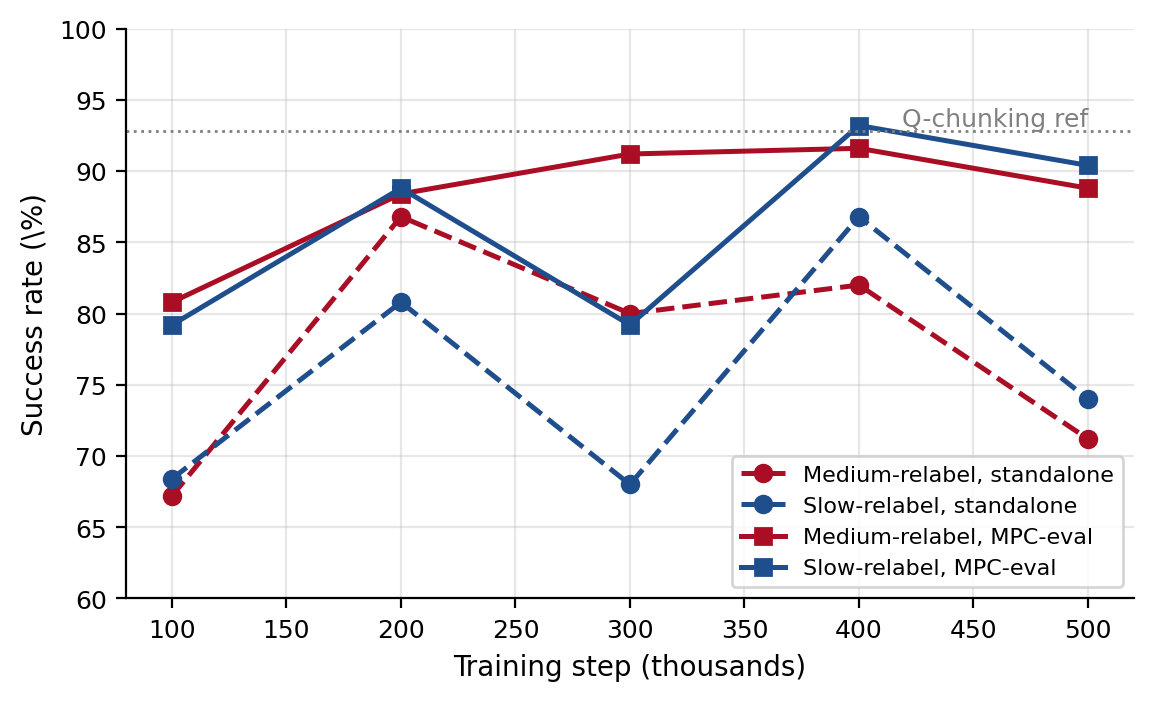
\includegraphics[width=0.85\linewidth]{figures/fmq_distil_curves.png}
\caption{Training curves for FMQ-label interleaved training.
Dashed lines show standalone success rate without world-model planning
at test time. Solid lines show MPC success rate after applying
Grad-MPC ($N=32$, $H=2$, $K=5$) to the trained actor. The slow
relabel schedule produces a cleaner peak of $93.2\%$ MPC success
at $400$k steps. The dotted line marks the Q-chunking reference
($92.8\%$).}
\label{fig:fmq-distil-curves}
\end{figure}

\begin{table}[h]
\centering
\caption{Effect of the FMQ relabelling interval during interleaved
MPC-based training. All runs use FMQ labels with
$\eta_{\mathrm{train}}=0.1$, $H=2$, $N=32$, and critic-update
probability $p=0.3$. Standalone SR evaluates the actor without the
world model. MPC SR applies Grad-MPC
($N=32$, $H=2$, $K=5$, Q-term) on top of the actor at each checkpoint.}
\label{tab:mpc-relabel-sweep}
\begin{tabular}{llrrrrr}
\toprule
Evaluation & Relabel Interval & 100k & 200k & 300k & 400k & 500k \\
\midrule
Standalone SR (\%) -- FMQ labels & 25k & 67.2 & \textbf{86.8} & 80.0 & 82.0 & 71.2 \\
Standalone SR (\%) -- FMQ labels & 50k & 68.4 & 80.8 & 68.0 & \textbf{86.8} & 74.0 \\
\midrule
MPC SR (\%) -- FMQ labels & 25k & 80.8 & 88.4 & 91.2 & 91.6 & 88.8 \\
MPC SR (\%) -- FMQ labels & 50k & 79.2 & 88.8 & 79.2 & \textbf{93.2} & 90.4 \\
\bottomrule
\end{tabular}
\end{table}

The medium relabelling schedule improves quickly but is less stable:
standalone success rises to $86.8\%$ at $200$k, then falls to
$71.2\%$ by $500$k. This suggests that frequent relabelling creates a
moving-target effect, where the actor and critic repeatedly adapt to
labels produced by a rapidly changing optimisation landscape.
The slow relabelling schedule is less aggressive but produces the best
checkpoint. At $400$k steps it reaches $86.8\%$ standalone success and
$93.2\%$ under MPC evaluation. This checkpoint is then used for the FMQ inference sweep below.
A full sweep over learning rate, buffer size, mix ratio, relabelling
interval, and trust-region radius, together with the early
high-frequency-relabel variants, is reported in
Appendix~\ref{app:oo-sweeps}.

\subsection{FMQ Inference after Learning from Generated Actions}
\label{sec:exp-fmq-distil-inf}

We now test whether FMQ-labelled training improves inference-time FMQ
planning. The key question is whether a critic trained on FMQ-shaped
actions remains reliable over a wider range of trust-region radii
$\eta$.
Table~\ref{tab:mpc-fmq-distilled} confirms this hypothesis. Unlike the
base critic in Table~\ref{tab:mpc-fmq-basepolicy}, which collapsed
rapidly for large $\eta$, the FMQ-trained critic remains above
$94.0\%$ success for $\eta \in [0.01,0.05]$ and reaches a peak success
rate of $96.0\%$ at both $\eta=0.02$ and $\eta=0.03$.

\begin{table}[h]
\centering
\caption{Inference-time planning on the FMQ-trained actor. The actor
is the $400$k checkpoint from the slow-relabel FMQ-trained run.
FMQ uses Q-all scoring unless stated otherwise. The broad high-performing
range of $\eta$ shows that the critic has become calibrated for
FMQ-shaped actions.}
\label{tab:mpc-fmq-distilled}
\begin{tabular}{lllr}
\toprule
Inference Method & Trajectory Score & Configuration & Success (\%) \\
\midrule
FMQ & Q-all  & $\eta = 0.01$ & 94.8 \\
FMQ & Q-all  & $\eta = 0.02$ & \textbf{96.0} \\
FMQ & Q-all  & $\eta = 0.03$ & \textbf{96.0} \\
FMQ & Q-all  & $\eta = 0.05$ & 94.0 \\
FMQ & Q-all  & $\eta = 0.10$ & 90.8 \\
FMQ & Q-all  & $\eta = 0.20$ & 80.8 \\
FMQ & Q-term & $\eta = 0.05$ & 93.6 \\
\midrule
Grad-MPC & Q-term & $K = 5$  & 93.2 \\
Grad-MPC & Q-term & $K = 8$  & \textbf{96.0} \\
Grad-MPC & Q-term & $K = 10$ & 90.8 \\
\midrule
Standalone trained actor & -- & $\mathrm{BoN}\,N=4$ & 86.8 \\
Q-chunking reference & -- & Published baseline & 92.8 \\
\bottomrule
\end{tabular}
\end{table}

This setting reaches a $96.0\%$ success rate, exceeding the Q-chunking
reference by $3.2$ percentage points and improving substantially over
the original $81.6\%$ offline checkpoint. Importantly, this improvement
does not come from using the world model as a training environment.
Instead, the world model is used in a controlled way: first to generate
planner-improved action labels, and then at inference time to make
short, trust-region-constrained action refinements.

\paragraph{Why Q-all works after FMQ-based training.}
The FMQ-trained rows use Q-all scoring by default. This differs from
the earlier frozen-policy MPC experiments, where Q-term was more robust.
The reason is that the critic has now been trained on FMQ-shaped actions
throughout the rollout, not only at the terminal state. Intermediate
critic values are therefore better calibrated, allowing Q-all to extract
more information from each imagined trajectory.
This isolates the role of critic calibration. Q-all is unreliable when
the critic has only seen dataset actions, but becomes useful once
interleaved training brings FMQ-modified actions into the critic's
training distribution.

\subsection{Actor Fine-Tuning with World-Model Transitions}
\label{sec:exp-mpc-online-wm}

The experiments above generate improved action targets but no new
state transitions. We next evaluate the online-in-WM procedure of
\S\ref{sec:mpcd-online-wm}, where FMQ-MPC rollouts inside the frozen
world model append imagined transitions to a replay buffer seeded with
offline data. We compare actor+critic updates against an actor-only
variant with the critic frozen, isolating whether imagined successors
can safely enter value learning.

\begin{table}[h]
\centering
\caption{Online fine-tuning with world-model-generated transitions on
\texttt{visual-cube-single-singletask-task1-v0}. All online runs use
FMQ-MPC inside the world model for $500{,}000$ steps
($N=32$, $H=2$, $\eta=0.02$, Q-all scoring). Success rate is measured
without a planner at test time over $250$ episodes, reported as mean
$\pm$ standard deviation over three seeds.}
\label{tab:mpc-online-e2}
\begin{tabular}{lcc}
\toprule
Method & Final Success (\%) & Peak Success (\%) \\
\midrule
Offline FQL checkpoint & 81.6 & 88.0 \\
Actor+critic update on imagined data & 30.7 $\pm$ 20.8 & 89.5 $\pm$ 0.7 \\
Actor-only update with frozen critic & \textbf{90.7 $\pm$ 0.8} & \textbf{94.8 $\pm$ 0.7} \\
\midrule
Frozen-critic checkpoint + FMQ-MPC at test time & -- & 93.2 $\pm$ 0.7 \\
\bottomrule
\end{tabular}
\end{table}

Table~\ref{tab:mpc-online-e2} and Figure~\ref{fig:online-in-wm-curves} show a sharp contrast between the two
training strategies. When the critic is updated on imagined transitions,
training initially improves but later collapses, ending at only
$30.7 \pm 20.8\%$ success. This mirrors the failure mode observed in
the world-model-as-environment experiments: once the critic is trained
on model-generated targets, value estimates become corrupted by
prediction error and, in the single-task setting, by the mismatch
between offline and generated reward scales. The actor then begins to
exploit those inaccuracies.
Freezing the critic prevents this collapse. The actor-only variant
improves smoothly, reaching a peak success rate of
$94.8 \pm 0.7\%$ and a final success rate of $90.7 \pm 0.8\%$. This is a
substantial improvement over the offline starting point, demonstrating
that imagined transitions can be useful when they are used as
policy-improvement data rather than as targets for critic learning.
Relative to the perfect-success latent-observation control in
Table~\ref{tab:owm-summary}, the frozen-critic method closes most of the
gap without additional real-environment interaction: the peak checkpoint
is only $5.2$ percentage points below the control.

\begin{figure}[h]
\centering
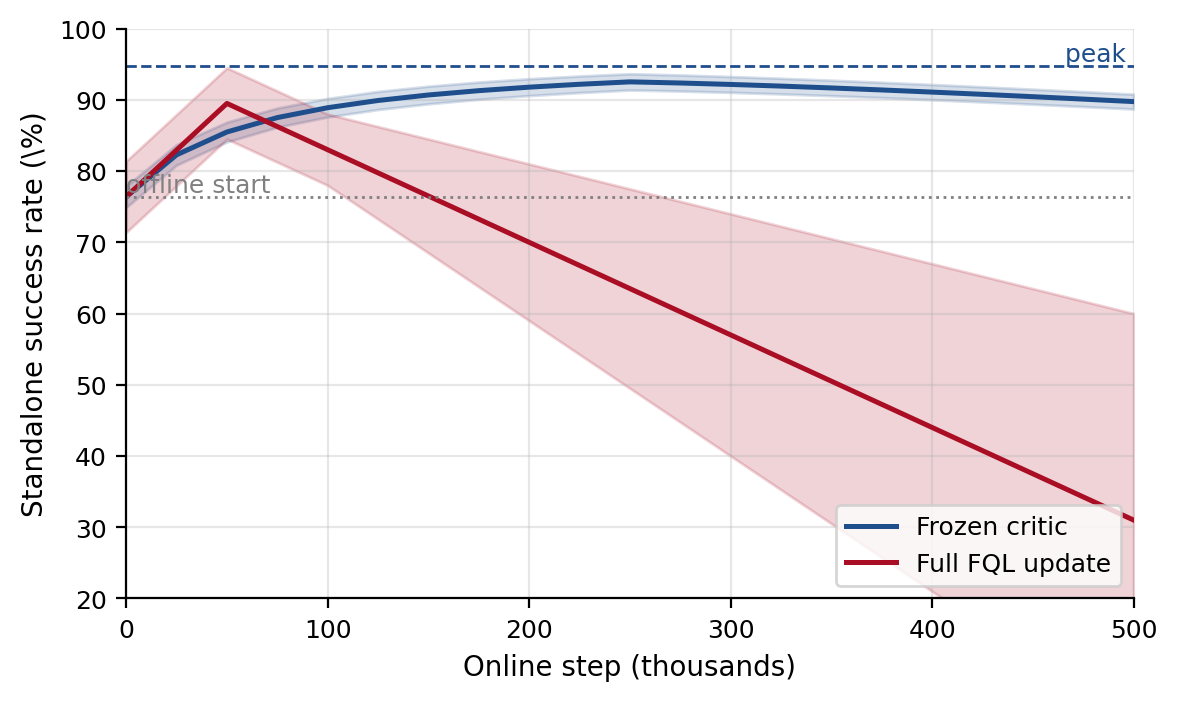
\includegraphics[width=0.85\linewidth]{figures/online_in_wm_curves.png}
\caption{Training trajectories for online fine-tuning inside the world
model. Both variants start from the same offline FQL checkpoint and use
the same FMQ-MPC planner to generate imagined transitions. Updating the
critic on imagined data leads to collapse after an early transient
improvement, whereas freezing the critic yields stable policy
improvement. Shaded regions show $\pm 1\sigma$ over three seeds.}
\label{fig:online-in-wm-curves}
\end{figure}

The final row of Table~\ref{tab:mpc-online-e2} applies the same FMQ-MPC
planner at test time on top of the best frozen-critic checkpoints. This
does not improve over the standalone actor peak
($93.2 \pm 0.7\%$ versus $94.8 \pm 0.7\%$). This suggests that the
actor has already absorbed most of the useful behaviour provided by the
planner during online fine-tuning. In other words, the world model has
served not as a reliable environment for critic learning, but as a
source of short-horizon policy-improvement supervision.
Thus, imagined transitions help only through an actor-only interface:
they provide useful policy-improvement data, but corrupt bootstrapped
value learning.

% ---------------------------------------------------------------------
\subsection{Goal-Conditioned Actor Fine-Tuning}
\label{sec:exp-mpc-online-wm-gc}

We now test the actor-only recipe in the full goal-conditioned setting
defined in \S\ref{sec:mpcd-gc}. The policy conditions on
$[z,z_{\mathrm{goal}}]$, training is shared across the five
\texttt{visual-cube-single} tasks, and rewards use the same
goal-conditioned indicator as offline pretraining. We compare direct
use of evaluation goals with achieved-state goals sampled from the
online buffer; the latter is the leakage-free protocol.

\begin{table}[h]
\centering
\caption{Goal-conditioned online fine-tuning inside the world model on
the five-task \texttt{visual-cube-single} benchmark. Success rate is
the standalone native OGBench success rate averaged over all five tasks
($50$ episodes per task), reported as mean $\pm$ standard deviation over
three seeds unless noted. The offline goal-conditioned baseline is
$90.0\%$.}
\label{tab:mpc-online-e3}
\begin{tabular}{llc}
\toprule
Online Training Variant & Goal Source & Final Success (\%) \\
\midrule
Offline goal-conditioned baseline & -- & 90.0 \\
\midrule
\multicolumn{3}{l}{\emph{Evaluation-goal training}} \\
HER relabelling, frozen critic & evaluation goals & 80.1 $\pm$ 1.6 \\
No HER relabelling, frozen critic & evaluation goals & 73.2 $\pm$ 1.2 \\
Mixed HER/no-HER (50/50), frozen critic & evaluation goals & 77.8 $\pm$ 3.0 \\
Mixed HER/no-HER (75/25), frozen critic & evaluation goals & 80.9 $\pm$ 1.5 \\
HER relabelling, updated critic & evaluation goals & 81.5 $\pm$ 1.3 \\
\midrule
\multicolumn{3}{l}{\emph{Achieved-state goal training}} \\
HER relabelling, frozen critic & achieved-state goals & 84.0 $\pm$ 1.5 \\
Mixed HER/no-HER (50/50), frozen critic & achieved-state goals & \textbf{84.4 $\pm$ 0.9} \\
\bottomrule
\end{tabular}
\end{table}

Table~\ref{tab:mpc-online-e3} shows that goal-conditioned
online-in-WM fine-tuning does not reliably improve over the offline
baseline. All final checkpoints fall below the $90.0\%$ offline policy,
including the variants that train directly on evaluation goals. The
strongest final results come from the leakage-free achieved-state
goal protocol: mixed HER/no-HER reaches $84.4 \pm 0.9\%$, and pure HER
reaches $84.0 \pm 1.5\%$. HER remains important, since the no-HER
evaluation-goal variant ends at only $73.2 \pm 1.2\%$.
The updated-critic row is also informative. Unlike the single-task
actor+critic update in Table~\ref{tab:mpc-online-e2}, it does not
collapse catastrophically: with the shared HIQL-style indicator reward,
updating the critic reaches $81.5 \pm 1.3\%$, close to the corresponding
frozen-critic evaluation-goal result of $80.1 \pm 1.6\%$. This supports
the interpretation that reward-scale mismatch was an important part of
the single-task critic-update failure, but it also shows that aligning
the reward scale is not sufficient to beat the offline baseline.
Unlike the single-task setting, freezing the critic is not sufficient to
produce a stable improvement. The likely reason is that the
goal-conditioned problem has substantially broader coverage
requirements. The actor must learn over the joint space
$(z,z_{\mathrm{goal}})$, and the online buffer generated by FMQ-MPC
covers only the narrow region visited by the current policy. As a
result, online fine-tuning tends to specialise the actor to the
distribution of imagined rollouts rather than improving performance
across the full benchmark.

% ---------------------------------------------------------------------
\subsection{Static World-Model Generated Dataset}
\label{sec:exp-wm-dataset-gen}

The previous experiments kept data generation coupled to the current
learner. We now evaluate the decoupled dataset-generation setting of
\S\ref{sec:mpcd-dataset-gen}: use the world model once to generate a
fixed synthetic corpus, then train offline RL methods without further
access to the model.

\paragraph{Setup.}
We compare three offline corpora, each containing approximately
$800$k goal-conditioned transitions across the five
\texttt{visual-cube-single} tasks:

\begin{itemize}
    \item \textbf{Real play data}: the original OGBench play dataset.
    \item \textbf{FMQ-generated data}: trajectories rolled out inside
    the world model using FMQ-MPC action selection
    ($N=32$, $H=2$, $\eta=0.02$).
    \item \textbf{BoN-generated data}: trajectories rolled out inside
    the world model using best-of-$N$ action selection without gradient
    refinement.
\end{itemize}

All corpora are stored without explicit goals: each transition contains
only latent states and actions, and goals are assigned during training
using the same HER sampler. This ensures that differences in downstream
performance come from the transition data itself, not from differences
in goal labelling.
We evaluate three downstream learners: FQL with a BC-flow actor, IQL
with AWR, and ReBRAC \cite{tarasov2023rebrac}. Performance is reported as the five-task native
success rate, averaged over three seeds.

\begin{table}[h]
\centering
\caption{Offline goal-conditioned learning from real and
world-model-generated corpora. Each corpus contains approximately
$800$k transitions and is processed with the same HER sampler during
training. \emph{Best Success} is the highest checkpoint over training;
\emph{Final Success} is the last checkpoint. Results are mean
$\pm$ standard deviation over three seeds.}
\label{tab:wm-dataset-gen}
\begin{tabular}{llrr}
\toprule
Learner & Training Corpus & Best Success (\%) & Final Success (\%) \\
\midrule
FQL (BC-flow actor) & Real play data & \textbf{90.3 $\pm$ 1.6} & 81.3 \\
FQL (BC-flow actor) & FMQ-generated data & 57.7 $\pm$ 3.8 & 41.7 \\
FQL (BC-flow actor) & BoN-generated data & 64.7 $\pm$ 3.7 & 55.7 \\
\midrule
IQL (AWR actor) & Real play data & 9.6 $\pm$ 1.8 & 5.3 \\
IQL (AWR actor) & FMQ-generated data & \textbf{16.4 $\pm$ 5.4} & 6.1 \\
IQL (AWR actor) & BoN-generated data & 16.0 $\pm$ 1.8 & 5.3 \\
\midrule
ReBRAC (TD3+BC actor) & Real play data & \textbf{13.7 $\pm$ 2.7} & 7.5 \\
ReBRAC (TD3+BC actor) & FMQ-generated data & 12.5 $\pm$ 3.4 & 5.7 \\
ReBRAC (TD3+BC actor) & BoN-generated data & 11.6 $\pm$ 1.4 & 6.7 \\
\bottomrule
\end{tabular}
\end{table}

Table~\ref{tab:wm-dataset-gen} shows that world-model-generated
datasets are substantially weaker than the original real play data for
the strongest downstream learner. FQL trained on real play reaches
$90.3 \pm 1.6\%$ best success, while the best synthetic corpus
(BoN-generated data) reaches only $64.7 \pm 3.7\%$. This gap persists
even though all corpora use the same HER procedure, indicating that the
limitation lies in the imagined trajectories themselves rather than in
the goal assignment process.
The comparison between FMQ-generated and BoN-generated data is also
informative. Although FMQ is the stronger online planner, it produces a
weaker offline dataset than BoN for FQL. This is because FMQ actions are
gradient-refined relative to the particular actor and critic used during
generation. When these actions are handed to a fresh learner, they no
longer arise from that learner's own policy distribution and are harder
to imitate. By contrast, BoN actions are unmodified samples from the
flow actor, making them more natural targets for a new flow-matching
policy.
The weaker performance of IQL and ReBRAC is less informative about the
datasets themselves. Both methods perform poorly across all corpora,
including real play data, suggesting that their policy classes and
training objectives struggle with the high-dimensional action chunks in
this benchmark. FQL is therefore the clearest indicator of corpus
quality.
Overall, the world model is not an adequate one-shot replacement for
real offline data. The useful signal in earlier sections depends on the
closed loop between the current actor, planner, and critic; once a fixed
synthetic corpus is handed to a fresh learner, much of that benefit is
lost.

% ---------------------------------------------------------------------
\section{World Model as Data Generator for New Environments}
\label{sec:exp-generalisation}

We next ask whether online-in-WM generalises beyond
\texttt{cube-single}. We evaluate two additional OGBench domains:
\texttt{visual-scene-play-v0}, which contains object-placement tasks in
a cluttered scene, and \texttt{visual-puzzle-3x3-play-v0}, which
contains button-configuration tasks on a $3\times3$ puzzle. In both
cases, a separate LeWM world model is trained from the corresponding
play dataset.

The key diagnostic is the \emph{action-conditioning ratio}: the factor
by which prediction error increases when the action sequence is
shuffled. High ratios indicate a steerable model; ratios near $1.0$
indicate that MPC has little basis for distinguishing action sequences.

\subsection{Action Conditioning as a Generalisation Diagnostic}
\label{sec:exp-gen-wm}

Before running the full RL pipeline, we measure the action-conditioning
ratio for each environment. This diagnostic is cheap to compute from
the latent cache and does not require pixel re-rendering or policy
training.

\begin{table}[h]
\centering
\caption{Action-conditioning ratio across environments. The ratio
measures how much prediction error increases when actions are shuffled
relative to the true action sequence. Larger values indicate that the
world model is more strongly action-conditioned and therefore more
suitable for MPC-based control.}
\label{tab:action-conditioning}
\begin{tabular}{lcc}
\toprule
Environment & Action-conditioning ratio & Expected online-in-WM effect \\
\midrule
\texttt{cube-single} & $8.0\times$ & strong improvement \\
\texttt{scene} & $1.4\times$ & small or marginal improvement \\
\texttt{puzzle-3x3} & $1.1\times$ & weak or harmful effect \\
\bottomrule
\end{tabular}
\end{table}

Table~\ref{tab:action-conditioning} shows that the three environments
span a wide range of action sensitivity. The cube environment has a
strongly action-conditioned world model, which is consistent with the
large gains observed earlier. In contrast, the scene and puzzle models
are only weakly action-conditioned. This suggests that MPC rollouts in
these environments may not reliably distinguish good actions from bad
ones, limiting the effectiveness of online-in-WM.
The remainder of this section tests whether this diagnostic predicts
the downstream RL results.

\subsection{Single-Task Online-in-WM}
\label{sec:exp-gen-single-task}

We first evaluate the single-task version of online-in-WM, matching the
protocol of \S\ref{sec:exp-mpc-online-wm}. The agent is trained for
$500$k FMQ-MPC steps inside the world model, using a frozen critic and
standalone evaluation without a planner at test time.

\begin{table}[h]
\centering
\caption{Single-task online-in-WM generalisation results. The method is
the frozen-critic online-in-WM procedure from
\S\ref{sec:exp-mpc-online-wm}, evaluated on task 1 of each environment.
Success is measured without a planner at test time over $250$
episodes.}
\label{tab:gen-single-task}
\begin{tabular}{lccc}
\toprule
Environment & Offline Success (\%) & Final Success (\%) & Peak Success (\%) \\
\midrule
\texttt{scene} & 18.8 & $17.1 \pm 2.4$ & $20.4 \pm 1.2$ \\
\texttt{puzzle-3x3} & 44.4 & 50.4 & 54.0 \\
\bottomrule
\end{tabular}
\end{table}

Table~\ref{tab:gen-single-task} reports these results. For \texttt{scene},
online-in-WM provides at most a marginal improvement. The peak success rate rises from $18.8\%$ to
$20.4 \pm 1.2\%$, but the final checkpoint falls slightly below the
offline baseline. This is consistent with the weak
$1.4\times$ action-conditioning ratio: the world model contains some
action information, but not enough to support strong policy
improvement.
The \texttt{puzzle-3x3} result is numerically positive, reaching
$54.0\%$ peak success from a $44.4\%$ offline baseline. However, this
environment has an action-conditioning ratio of only $1.1\times$, so
the result should be interpreted cautiously. The world model is nearly
action-agnostic, and the online curve is correspondingly high variance.
The result is therefore best viewed as a weak positive signal rather
than strong evidence of robust generalisation.
Overall, the single-task results are much weaker than those observed on
\texttt{cube-single}. This already suggests that online-in-WM depends
strongly on the steerability of the learned dynamics model.

\subsection{Goal-Conditioned Online-in-WM}
\label{sec:exp-gen-goal-conditioned}

We next evaluate the full goal-conditioned setting. This is the harder
test: the policy must generalise across all five tasks, conditions on
both the current latent state and the goal latent, and uses HER during
online fine-tuning. The protocol matches
\S\ref{sec:exp-mpc-online-wm-gc}.

\begin{table}[h]
\centering
\caption{Goal-conditioned online-in-WM generalisation results.
Performance is averaged across all five tasks, with $50$ evaluation
episodes per task. Success is measured without a planner at test time.}
\label{tab:gen-goal-conditioned}
\begin{tabular}{lccc}
\toprule
Environment & Offline Success (\%) & Final Success (\%) & Peak Success (\%) \\
\midrule
\texttt{scene} & 8.4 & $8.4 \pm 0.6$ & $10.7 \pm 1.0$ \\
\texttt{puzzle-3x3} & 3.2 & 0.8 & 3.6 \\
\bottomrule
\end{tabular}
\end{table}

Table~\ref{tab:gen-goal-conditioned} reports the goal-conditioned results,
which are weaker than the single-task results.
For \texttt{scene}, online-in-WM matches the offline baseline at the
final checkpoint and reaches only a small peak improvement of
$10.7 \pm 1.0\%$. For \texttt{puzzle-3x3}, performance decreases:
the final success rate falls from $3.2\%$ to $0.8\%$, and the best
checkpoint only recovers to $3.6\%$.
The per-task breakdown in Table~\ref{tab:gen-goal-conditioned-tasks}
shows why the five-task average remains low. In both environments,
non-zero success is concentrated almost entirely on task 1, while tasks
2--5 remain unsolved. The online-in-WM phase therefore does not
discover broad goal-conditioned competence; it mainly reinforces the
easiest part of the task distribution.

\begin{table}[h]
\centering
\caption{Per-task final success rates for goal-conditioned
online-in-WM. Success is concentrated on task 1; tasks 2--5 remain at
$0\%$ throughout training in both environments.}
\label{tab:gen-goal-conditioned-tasks}
\begin{tabular}{lrrrrrr}
\toprule
Environment & Task 1 & Task 2 & Task 3 & Task 4 & Task 5 & Average \\
\midrule
\texttt{scene} & $\sim 41.0$ & 0.0 & 0.0 & 0.0 & 0.0 & 8.4 \\
\texttt{puzzle-3x3} & 4.0 & 0.0 & 0.0 & 0.0 & 0.0 & 0.8 \\
\bottomrule
\end{tabular}
\end{table}

These results indicate that the goal-conditioned setting is more
sensitive to weak action conditioning than the single-task setting. The
policy must cover a larger input space, since observations contain both
the current latent state and the goal latent. In addition, successful
online updates require the MPC controller to generate transitions that
move specifically toward the requested goal, not merely plausible
transitions under the world model. When the predictor is weakly
action-conditioned, imagined rollouts do not reliably reflect
goal-directed consequences of actions, and the generated buffer becomes
too noisy to improve the policy.

\paragraph{Summary.}
The three-environment comparison points to a simple regularity:
action conditioning appears to be necessary for online-in-WM to work.
On \texttt{cube-single}, where the action-conditioning ratio is
$8.0\times$, the method produces a large improvement. On
\texttt{scene}, where the ratio is only $1.4\times$, gains are small.
On \texttt{puzzle-3x3}, where the ratio is $1.1\times$, the
goal-conditioned method is ineffective or harmful.
This diagnostic is useful because it can be computed cheaply before
running the full RL pipeline. In practice, it provides a screening test
for whether a learned world model is likely to be steerable enough to
support MPC-based online fine-tuning.

% ---------------------------------------------------------------------
\section{Latent Subgoal Planning Results}
\label{sec:exp-wm-as-subgoal}

The final experiments evaluate Latent Subgoal Planning (LSP), introduced
in Chapter~\ref{chap:wm-as-subgoal}. LSP uses the world model at the
high level: Phase 1 trains a purely offline hierarchy, while Phase 2
freezes the low-level controller and value function and updates only
the high-level subgoal policy.

\subsection{Offline Hierarchical Baseline}
\label{sec:exp-lsp-phase1}

Phase 1 establishes the offline LSP baseline. It replaces the Gaussian
high- and low-level policies of HIQL with flow-matching actors, but uses
no world-model rollouts during training.

\begin{table}[h]
\centering
\caption{Offline hierarchical baseline on OGBench
\texttt{cube-single}. LSP Phase 1 replaces the Gaussian high- and
low-level policies of HIQL with flow-matching policies while remaining
purely offline. Success rate is the native five-task average.}
\label{tab:lsp-phase1}
\begin{tabular}{lr}
\toprule
Method & Success (\%) \\
\midrule
HIQL end-to-end & 87.0 \\
LSP Phase 1 (flow HL + flow LL) & \textbf{88.0} \\
\bottomrule
\end{tabular}
\end{table}

Table~\ref{tab:lsp-phase1} shows that the Phase-1 LSP baseline is
already competitive with end-to-end HIQL, slightly improving the
five-task average from $87.0\%$ to $88.0\%$. The remaining experiments
therefore test whether the world model can improve an already strong
offline hierarchy, rather than rescuing a weak baseline.

\subsection{World-Model-Grounded AWR}
\label{sec:exp-phase2-awr}

Table~\ref{tab:lsp-phase2-awr} evaluates the Phase-2 AWR update from
\S\ref{sec:lsp-awr-data}, sweeping the temperature $\alpha$. The frozen
high-level control checks whether Phase-1 performance is preserved, and
the offline AWR control isolates the effect of the high-level update
from world-model rollout error.

\begin{table}[h]
\centering
\caption{Phase-2 high-level AWR updates on OGBench
\texttt{cube-single}. Step-0 is the Phase-1 checkpoint at the start of
Phase 2. Peak is the best evaluation checkpoint, and final is the
checkpoint after $500{,}000$ updates. All runs freeze the low-level
policy.}
\label{tab:lsp-phase2-awr}
\begin{tabular}{llrrr}
\toprule
Update Type & $\alpha$ & Step-0 (\%) & Peak (\%) & Final (\%) \\
\midrule
No high-level update & --  & 85 & 89 & 87 \\
\midrule
World-model AWR & 5.0  & 77 & 88 & 79 \\
World-model AWR & 2.0  & 82 & 84 & 76 \\
World-model AWR & 1.0  & 83 & 71 & 54 \\
World-model AWR & 0.5  & 80 & 39 & 29 \\
World-model AWR & 0.1  & 88 & 12 & 6 \\
\midrule
Offline AWR control & 2.0  & 81 & 92 & 63 \\
Offline AWR control & 1.0  & 83 & 73 & 60 \\
Offline AWR control & 0.1  & 80 & 15 & 6 \\
\bottomrule
\end{tabular}
\end{table}

The frozen high-level control preserves performance, ending at
$87\%$. This confirms that degradation is not caused by the evaluation
protocol; it appears only when
the high-level policy is updated.
The world-model AWR rows show no reliable improvement over Phase 1.
At high temperature ($\alpha=5.0$), the update is highly selective and
performance is mostly preserved, reaching $88\%$ peak but falling to
$79\%$ final. As $\alpha$ decreases, the update spreads probability mass
over a broader set of subgoal targets and performance degrades rapidly,
collapsing to $6\%$ final at $\alpha=0.1$.
The offline AWR control shows the same pattern. Even without world-model
rollouts, updating the high-level flow policy toward broad dataset
subgoal targets destabilises the hierarchy. The $\alpha=2.0$ offline
control briefly reaches $92\%$, but this is not stable and falls to
$63\%$ by the final checkpoint. This suggests that the core failure is
not simply inaccurate world-model evaluation. Instead, the high-level
AWR update changes the subgoal distribution in a way that the frozen
low-level policy cannot reliably follow. In effect, the update
de-sharpens a strong Phase-1 high-level policy rather than improving it.

\subsection{AWR with Achieved Latent States}
\label{sec:exp-phase2-hrf}

Table~\ref{tab:lsp-hrf} evaluates Hindsight Reality Forcing (HRF), the
achieved-state variant introduced in \S\ref{sec:lsp-hrf}. HRF tests
whether replacing proposed subgoals with rollout endpoints avoids the
value-gaming failure mode of AWR.

\begin{table}[h]
\centering
\caption{Phase-2 Hindsight Reality Forcing (HRF). Step-0 is the
Phase-1 baseline. HRF replaces proposed-subgoal targets with the latent
states achieved after world-model rollouts.}
\label{tab:lsp-hrf}
\begin{tabular}{llrrrr}
\toprule
Update Type & Low-Level Policy & Step-0 (\%) & 50k (\%) & 100k (\%) & 500k (\%) \\
\midrule
HRF, $\alpha=1.0$ & frozen  & 82 & 0 & 0 & 0 \\
HRF, $\alpha=3.0$ & frozen  & 88 & 0 & 1 & 0 \\
HRF, $\alpha=1.0$ & updated & 80 & 0 & 0 & 0 \\
\bottomrule
\end{tabular}
\end{table}

HRF fails immediately. All configurations collapse to approximately
zero success by the first evaluation checkpoint at $50$k steps. This
shows that the problem is not only value gaming. Even when the update
is forced to imitate the achieved rollout endpoint, the resulting
targets occupy a distribution that differs from the dataset subgoals on
which the low-level policy was trained.
Updating the low-level policy alongside the high-level policy does not
solve the issue. Once the high-level distribution shifts, the low-level
targets shift with it, and the hierarchy loses the coordination learned
during Phase 1.
The LSP experiments are therefore a negative result. Phase 1 gives a
strong offline hierarchy, but both AWR and HRF destabilise it once the
high-level subgoal distribution shifts away from the distribution on
which the low-level policy was trained.
Further Phase-2 ablations --- the low-level reachability metric,
low-level freezing, high-level update cadence, and an alternative
real-candidate grounding mode --- are reported in
Appendix~\ref{app:lsp-ablations}.

% ---------------------------------------------------------------------
\section{Headline Results and Empirical Findings}
\label{sec:exp-headline}

This section collects the main empirical results and the two findings
that explain the overall pattern.

\begin{table}[h]
\centering
\caption{Headline comparison across the main experimental settings.
Single-task results are evaluated on
\texttt{visual-cube-single-singletask-task1-v0} over $250$ episodes.
Goal-conditioned results are five-task native OGBench averages. The
table reports the best representative result for each method family.}
\label{tab:headline}
\begin{tabular}{llc}
\toprule
Method & Setting & Success (\%) \\
\midrule
\multicolumn{3}{l}{\emph{Offline and non-WM baselines}} \\
Offline FQL checkpoint & single-task & 81.6 \\
Q-chunking reference & single-task & 92.8 \\
HIQL end-to-end & goal-conditioned, 5 tasks & 87.0 \\
\midrule
\multicolumn{3}{l}{\emph{World model as a training environment}} \\
World Model RL (Sparse Reward, 3 seeds) & single-task & $24.5 \pm 5.1$ \\
Anchored World Model RL (Dense Reward) & single-task & 15.2 \\
Joint Predictor--Policy Training & single-task & 9.6 \\
Nearest-Neighbour Regularisation & single-task & 2.4 \\
\midrule
\multicolumn{3}{l}{\emph{Inference-time planning with a frozen policy}} \\
BoN-MPC, $H=1$ & single-task & 88.0 \\
Grad-MPC, $H=2$, $K=5$ & single-task & 90.0 \\
FMQ on frozen critic, $\eta=0.1$ & single-task & 90.0 \\
\midrule
\multicolumn{3}{l}{\emph{Policy learning from MPC-generated data and calibrated inference}} \\
Grad-MPC interleaved training, critic-update setting & single-task & 92.4 \\
FMQ-trained actor + FMQ inference & single-task & \textbf{96.0} \\
FMQ-trained actor + Grad-MPC inference, $K=8$ & single-task & \textbf{96.0} \\
\midrule
\multicolumn{3}{l}{\emph{Online fine-tuning inside the world model}} \\
Online-in-WM, actor+critic update & single-task & 30.7 $\pm$ 20.8 \\
Online-in-WM, frozen critic (final) & single-task & 90.7 $\pm$ 0.8 \\
Online-in-WM, frozen critic (peak) & single-task & \textbf{94.8 $\pm$ 0.7} \\
Goal-conditioned online-in-WM, achieved-state goals (final) & goal-conditioned, 5 tasks & 84.4 $\pm$ 0.9 \\
\midrule
\multicolumn{3}{l}{\emph{Latent Subgoal Planning}} \\
LSP Phase 1 (flow HL + flow LL) & goal-conditioned, 5 tasks & \textbf{88.0} \\
LSP Phase 2, World-model AWR, best final & goal-conditioned, 5 tasks & 79.0 \\
LSP Phase 2, Hindsight Reality Forcing & goal-conditioned, 5 tasks & $\approx 0$ \\
\midrule
\multicolumn{3}{l}{\emph{Generalisation to new environments}} \\
Single-task online-in-WM, \texttt{scene}  & single-task & 20.4 $\pm$ 1.2 \\
Single-task online-in-WM, \texttt{puzzle-3x3} & single-task & 54.0 \\
Goal-conditioned online-in-WM, \texttt{scene}  & goal-conditioned, 5 tasks & 10.7 $\pm$ 1.0 \\
Goal-conditioned online-in-WM, \texttt{puzzle-3x3} & goal-conditioned, 5 tasks & 3.6 \\
\bottomrule
\end{tabular}
\end{table}

Table~\ref{tab:headline} shows the main pattern. The weakest results
come from treating the world model as a replacement environment; the
strongest single-task results come from local planning,
planner-generated action supervision, and actor-only online-in-WM. The
goal-conditioned results are more limited: LSP Phase 1 is the strongest
stable five-task method, but Phase 2 world-model updates and
goal-conditioned online-in-WM do not reliably beat the offline
baselines.

\paragraph{Finding 1: the offline critic is the most reliable bridge
between imagined rollouts and real task success.}
The most successful methods use LeWM to generate candidate futures and
the offline critic to choose among them. This matters because the critic
is better aligned with native task success than latent distance alone:
CEM reaches the goal embedding with $0.0\%$ native success, whereas
BoN-MPC, Grad-MPC, and FMQ improve by ranking candidates with the
real-data critic. Once imagined successors enter Bellman targets,
however, prediction error can corrupt the critic itself.

\paragraph{Finding 2: world models are useful locally, but unreliable
as long-horizon training environments.}
One- and two-step planning improves performance, and gradient-based
action refinement provides additional gains. Longer imagined training
loops are much less reliable: prediction drift corrupts value learning,
static synthetic corpora underperform real play data, and Phase-2 LSP
updates create a subgoal distribution shift that the frozen low-level
policy cannot absorb. The consistent positive case is therefore local:
LeWM proposes short-horizon improvements, the offline critic selects
among them, and the actor absorbs the improvement without rewriting the
value function.

% ---------------------------------------------------------------------
\section{Limitations and Threats to Validity}
\label{sec:exp-threats}

The results in this chapter give a consistent picture, but they should
not be read as a complete statement about all latent world models or all
offline RL settings. The strongest single-task results come from one
OGBench domain, and each environment is evaluated with one frozen LeWM
checkpoint. The cross-environment experiments in
\S\ref{sec:exp-generalisation} make this less narrow by testing where
the recipe transfers, but they do not remove the dependence on the
particular model family used here. A world model with different training
data, architecture, or long-horizon accuracy could change where the
boundary lies between useful short-horizon prediction and harmful model
exploitation.

The experimental coverage is also uneven. The online-in-WM comparisons
use three or four seeds, but several inference-time MPC sweeps
(Tables~\ref{tab:mpc-bon}--\ref{tab:mpc-fmq-distilled}) and the LSP
Phase-2 experiments are single runs evaluated over many episodes. The
$96.0\%$ result is also the best checkpoint from a sweep, so it is best
viewed as evidence that the method can reach that level, not as a fully
seeded estimate of its expected performance. This is why final
checkpoints are reported alongside peak checkpoints where possible:
final performance is the fairer measure when no real-environment
validation signal should be available during deployment.

Comparisons with external baselines should be interpreted with similar
care. The methods in this thesis were tuned through the sweeps in
Appendix~\ref{app:oo-sweeps}, while the Q-chunking reference value of
$92.8\%$ is a published number obtained under a separate tuning budget.
The comparison is still useful as a reference point, but the margin over
Q-chunking should not be treated as a perfectly controlled benchmark
comparison.

There is also a leakage issue in some of the goal-conditioned
experiments. Variants that train directly on evaluation goals are useful
diagnostics, because they show what happens when the intended goal
distribution is given to the online-in-WM loop. They are not, however,
the cleanest protocol. For that reason, the achieved-state goal results
in \S\ref{sec:exp-mpc-online-wm-gc} are the main leakage-free numbers,
and the conclusions about goal-conditioned online-in-WM are based on
those results.

Finally, the most successful online-in-WM method relies heavily on the
offline critic. The same critic scores MPC candidates and provides the
training signal for the actor, so any systematic critic error could be
reinforced rather than corrected. The real-environment gains suggest
that this was not the dominant failure mode on the benchmarks studied,
but the method still depends on the critic being better grounded than
the world model predictions it evaluates.


\chapter{Conclusion}
\label{chap:conclusion}

\section{Summary of Findings}
\label{sec:concl-summary}

This thesis investigated how a frozen latent world model can be used to
improve offline reinforcement learning for high-dimensional robotic
manipulation. We evaluated a latent action-conditioned world model in several roles: as
a training environment, as a short-horizon planner, as a source of
world-model-generated training data, and as a tool for grounding
hierarchical subgoals. The central finding is that these roles are not
equivalent. The world model is useful when used locally and
conservatively, but unreliable when treated as a replacement for the
environment or as an unconstrained source of training data.

Using the world model as a surrogate environment for reinforcement
learning consistently failed to improve over the offline baseline.
Across sparse rewards, dense rewards, anchoring, joint
predictor--policy training, uncertainty penalties, and
nearest-neighbour regularisation, policy optimisation inside the
learned dynamics either underperformed or collapsed. The failure mode is
consistent with the predictor-drift analysis: small latent prediction
errors accumulate over rollout horizons, and once the critic is allowed
to bootstrap on imagined successors, value estimates become corrupted.
This shows that accurate short-horizon prediction is not sufficient for
stable long-horizon reinforcement learning inside a learned simulator.

In contrast, the world model is useful for short-horizon
value-guided planning. Best-of-$N$ MPC improves the single-task offline
policy from $81.6\%$ to $88.0\%$, and gradient-based value-guided
planning reaches $90.0\%$ with no parameter updates. FMQ achieves the
same level on the frozen offline critic, but only within a narrow
trust-region range. After training the actor and critic on
planner-generated actions, FMQ inference becomes substantially more
robust and reaches $96.0\%$ success. This result highlights the key
mechanism: the planner benefits from the world model's local
counterfactual predictions, but only when the critic remains calibrated
to the actions being evaluated.

The online-in-WM experiments provide the clearest evidence for how
imagined transitions should be used during training. Updating both actor
and critic on world-model-generated transitions collapses to
$30.7 \pm 20.8\%$. Freezing the critic and updating only the actor
instead reaches a standalone peak of $94.8 \pm 0.7\%$ and a final
success rate of $90.7 \pm 0.8\%$ on the single-task benchmark. The
world model can therefore provide useful policy-improvement
supervision, but should not be used to generate bootstrapping targets
for value learning.

The same recipe does not transfer cleanly to the full
goal-conditioned benchmark. Goal-conditioned online-in-WM briefly
matches or exceeds the offline baseline, but final performance remains
below it; the strongest leakage-free achieved-state-goal variant reaches
$84.4 \pm 0.9\%$ compared with a $90.0\%$ offline baseline. Generating a
fixed offline corpus from the world model also underperforms real play
data: with identical HER processing, FQL reaches $90.3 \pm 1.6\%$ on
real data but only $64.7 \pm 3.7\%$ on the best world-model-generated
corpus. These results suggest that the successful single-task methods
depend on closed-loop interaction between the current actor, planner,
and frozen critic. Once that loop is broken, much of the benefit is
lost.

Latent Subgoal Planning (LSP) provides the strongest stable
goal-conditioned result. Phase 1, trained entirely offline with
flow-matching high- and low-level policies, reaches $88.0\%$ on the
five-task benchmark, slightly exceeding the HIQL end-to-end baseline.
However, Phase 2 attempts to improve the high-level policy using
world-model-grounded AWR or achieved-state subgoal regression do not
surpass this baseline. Conservative updates preserve some Phase-1
performance but do not improve it, while more aggressive updates
collapse the hierarchy. The likely cause is distributional coupling:
shifting the high-level subgoal distribution pushes the frozen low-level
policy outside the conditioning distribution it was trained to execute.

Several early SAC-based approaches, including curriculum SAC, HER+SAC,
and hierarchical SAC with expert-guided stabilisation, were also
explored. These methods could often optimise latent-reaching objectives
inside the world model, but did not transfer to native task success in
MuJoCo. They are therefore treated as exploratory negative results and
documented separately in the appendix.

Overall, the thesis supports a constrained view of learned world models
for offline robotic control. The world model is not reliable enough to
serve as a standalone simulator, a replacement offline dataset, or an
unconstrained subgoal generator. Its strength lies in short-horizon,
local counterfactual reasoning. When paired with a critic trained on
real transitions, this local reasoning can improve action selection,
generate useful actor-training data, and produce substantial gains in
single-task manipulation.

\section{Future Work}
\label{sec:concl-future}

\paragraph{Improving world-model reliability and action conditioning.}
The methods that succeed in this thesis all avoid long-horizon open-loop
rollouts. They use the world model over one or two prediction steps and
rely on a critic trained on real data to score the result. Future work
should repeat the same diagnostic pipeline with world-model
architectures that may offer longer reliable horizons or stronger action
conditioning, such as diffusion-transformer world models,
Dreamer-style recurrent state-space models, or value-aware latent
models. The action-conditioning ratio used in the generalisation
experiments is also a useful pre-screening diagnostic: online-in-WM
should only be expected to help when the learned dynamics are
sufficiently sensitive to actions.

\paragraph{Scaling generated-data methods to goal-conditioned control.}
The single-task online-in-WM method improves substantially, but the
goal-conditioned extension does not reliably beat the offline baseline.
Future work should focus on coverage: more diverse goal sampling,
explicit exploration bonuses in the MPC scorer, higher weighting of
real offline replay during online updates, or goal-conditioned critics
specialised to different regions of the goal space. These directions
target the main weakness observed here: the generated online buffer
becomes concentrated around the states visited by the current planner,
rather than covering the full state-goal distribution.

\paragraph{Stabilising hierarchical world-model learning.}
The LSP Phase-2 failures leave a clear open problem: how can a
hierarchical policy use world-model-derived supervision without breaking
coordination between the high and low levels? In the flat single-task
case, the successful rule is to freeze the critic and update only the
actor. The analogous rule for hierarchical agents is less obvious,
because changing the high-level policy also changes the conditioning
distribution faced by the low-level policy. Future work could explore
conservative subgoal trust regions, explicit low-level reachability
models, or joint update rules that maintain compatibility between
proposed subgoals and low-level competence. The broader challenge is to extend the local usefulness of learned
world models to broader goal-conditioned and hierarchical settings
without losing the grounding provided by real experience.



\bibliographystyle{vancouver}
\bibliography{bibs/sample}

\chapter{Declarations}
\label{chap:declarations}

\section{Use of Generative AI}
\label{sec:decl-ai}

I acknowledge the use of GPT-5.5 (https://chatgpt.com/) to support the editing of this report. In particular, it was used to help improve existing wording, restructure sections and refine the presentation of tables and figures. I also used Claude Opus 4.7 (https://claude.ai/) to assist with experiment code, debugging, and the generation of figures and tables.

All technical decisions, experimental design choices, implementation decisions, and final interpretations of results remain my own. Outputs from generative AI tools were reviewed, edited, and verified before inclusion. I confirm that no AI-generated content has been presented as my own independent work.

\section{Ethical Considerations}
\label{sec:decl-ethics}

This project does not involve human participants, patient data, personally identifiable information, or sensitive personal data. The experiments are conducted using publicly available or research-standard reinforcement learning benchmarks and simulated robotic environments. As such, the project does not raise the same data privacy or consent concerns associated with studies involving human subjects.

The main ethical considerations relate to responsible reporting of results and the limitations of simulated robotics research. Policies trained in simulation may not transfer safely to real robotic systems without further validation, particularly where physical interaction, contact dynamics, or unsafe exploration could cause damage. For this reason, all claims in this thesis are limited to the simulated benchmark settings evaluated, and no claim is made that the learned policies are safe for direct deployment on real robotic hardware.

\section{Sustainability}
\label{sec:decl-sustainability}

This project required the use of GPU compute for training world-model-based reinforcement learning agents and running evaluation experiments. I made efforts to reduce unnecessary computation where possible. In particular, pretrained or frozen representations were reused across experiments, cached latent datasets were used to avoid repeated image encoding, and evaluation was generally performed at fixed checkpoints rather than continuously. Several experiments also reused offline buffers and saved checkpoints rather than retraining complete pipelines from scratch.

Despite these efforts, the project involved a significant number of GPU training runs due to the experimental nature of reinforcement learning research and the need to compare multiple methods, ablations, and random seeds. The sustainability impact of this compute usage is acknowledged as a limitation of the work.

\section{Availability of Data and Materials}
\label{sec:decl-availability}

The project materials are available as follows:

\begin{itemize}
    \item Project source code: \url{https://github.com/jdefreitas02/latent-subgoal-chaining}.
    \item Benchmark environments and datasets: experiments are based on the OGBench simulated robotic manipulation benchmarks.
    \item The official LeWM checkpoints can be found on Hugging Face here \url{https://huggingface.co/papers/2603.19312}. Generated datasets, and experiment outputs can be reproduced by following the instructions provided in the project repository.
\end{itemize}

\appendix
\chapter{First Appendix}

\section{Offline-to-Online Hyperparameter Sweeps}
\label{app:oo-sweeps}

The tables below collect the full hyperparameter sweeps referenced in
Chapter~\ref{chap:mpc-distill}. All entries use the same environment
(\texttt{visual-cube-single-singletask-task1-v0}, $250$ episodes per
evaluation) and the same offline policy starting point
(\texttt{sd55445}, $81.6\%$).

\begin{table}[h]
\centering
\caption{FMQ-label early variants (D7a, D7b) at a $10$k relabeling
   interval. The high-frequency relabeling causes oscillation: D7a
   reaches $90.0\%$ standalone at $200$k but the checkpoint was not
   saved, and the final-checkpoint MPC-eval matches the D4 Grad-MPC
   baseline.}
\label{tab:app-d7ab}
\begin{tabular}{l l r l}
\toprule
Run & Mode & Final SA (\%) & MPC-eval (\%) \\
\midrule
D7a (FMQ mixed)     & mixed     & 72.8 & 92.4 (Grad-MPC $K{=}5$); 86.8 (FMQ $\eta{=}0.1$) \\
D7b (FMQ mixed-awr) & mixed-awr & 75.6 & 88.8 (Grad-MPC $K{=}5$); 86.4 (FMQ $\eta{=}0.1$) \\
\bottomrule
\end{tabular}

\medskip
\noindent\textbf{D7a standalone progression} (eval every $100$k steps):
$100$k:~$70.4\%$, \textbf{$200$k:~$90.0\%$}, $300$k:~$77.6\%$,
$400$k:~$81.6\%$, $500$k:~$72.8\%$. The $200$k peak was lost due to
missing intermediate checkpoints; this bug was fixed in all subsequent
runs (D7c onwards).
\end{table}

\begin{table}[h]
\centering
\caption{Training hyperparameter sweep (D7e--D7p). All runs use FMQ
   label generation at $\eta_{\text{train}}$, mixed injection,
   eval+checkpoint every $25$k. Baseline (D7d): $\mathrm{lr}{=}3\times
   10^{-4}$, $\mathrm{mix}{=}0.3$, $\mathrm{relabel}{=}50$k,
   $\mathrm{buf}{=}2000$, $\mathrm{warmup}{=}100$k,
   $\eta_{\text{train}}{=}0.1$, seed $42$. ``Peak SA'' is the highest
   standalone success rate ($\mathrm{BoN}\,N{=}4$) across all saved
   checkpoints. D7e/D7n/D7o/D7p were run for $300$k steps; the rest are
   $500$k.}
\label{tab:app-d7-train-sweep}
\begin{tabular}{l l l l l l l l}
\toprule
Run & lr & mix & relabel & buf & warmup & $\eta_{\text{train}}$ & Peak SA (\%) \\
\midrule
\multicolumn{8}{l}{\emph{Relabeling interval / buffer / mix ratio variants}} \\
D7f & $3{\times}10^{-4}$ & 0.5 & 10k & 2000 & 100k & 0.10 & 82.4 \\
D7g & $3{\times}10^{-4}$ & 0.5 & 25k & 2000 & 100k & 0.10 & 86.4 \\
D7h & $3{\times}10^{-4}$ & 0.3 & 10k & 2000 &  50k & 0.10 & 86.0 \\
D7i & $3{\times}10^{-4}$ & 0.3 & 10k &  500 & 100k & 0.10 & 82.4 \\
D7j & $3{\times}10^{-4}$ & 0.3 & 50k & 5000 & 100k & 0.10 & 89.2 \\
D7k & $3{\times}10^{-4}$ & 0.3 & 10k & 2000 & 100k & 0.05 & 88.0 \\
D7l & $3{\times}10^{-4}$ & 0.3 & 10k & 2000 & 100k & 0.10 & 88.0 \\
D7m & $3{\times}10^{-4}$ & 0.5 & 10k &  500 & 100k & 0.10 & 84.0 \\
\midrule
\multicolumn{8}{l}{\emph{Lower learning-rate variants}} \\
D7e & $3{\times}10^{-4}$ & 0.3 & 10k & 2000 & 100k & 0.10 & 87.6 (at 150k) \\
D7n & $1{\times}10^{-4}$ & 0.3 & 50k & 2000 & 100k & 0.10 & 86.0 \\
D7o & $5{\times}10^{-5}$ & 0.3 & 50k & 2000 & 100k & 0.10 & 81.2 \\
D7p & $1{\times}10^{-4}$ & 0.5 & 50k & 2000 & 100k & 0.10 & \textbf{90.0 (at 275k)} \\
\bottomrule
\end{tabular}

\medskip
\noindent\textbf{Key takeaways.} Buffer size has the largest single
effect: D7j ($\mathrm{buf}{=}5000$, peak $89.2\%$) vs.\ D7i
($\mathrm{buf}{=}500$, $82.4\%$) is a $+6.8\%$ absolute lift. A lower
learning rate paired with a stronger mix ratio (D7p) produces the
cleanest single peak ($90.0\%$ at $275$k), suggesting reduced
oscillation lets the training maintain the peak. The very low learning
rate $5\times 10^{-5}$ (D7o) underperforms: too slow even at $300$k.
\end{table}

\begin{table}[h]
\centering
\caption{FMQ ($\eta=0.02$, $H=2$, $J_{\text{Q-all}}$, $N=32$)
   evaluation on the best-of-each-run standalone checkpoints. Pending
   evaluations are marked ``--''.}
\label{tab:app-d7-fmq002}
\begin{tabular}{l l r r}
\toprule
Run & Checkpoint & Standalone SR (\%) & FMQ $\eta{=}0.02$ SR (\%) \\
\midrule
D7p & \texttt{params\_275000.pkl} & 90.0 & -- \\
D7j & \texttt{params\_300000.pkl} & 89.2 & -- \\
D7k & \texttt{params\_200000.pkl} & 88.0 & -- \\
D7l & \texttt{params\_275000.pkl} & 88.0 & -- \\
D7e & \texttt{params\_150000.pkl} & 87.6 & -- \\
D7d & \texttt{params\_400000.pkl} & 86.8 & 96.0 (ref., Table~\ref{tab:mpc-fmq-distilled}) \\
\bottomrule
\end{tabular}
\end{table}

\begin{table}[h]
\centering
\caption{D7q combined-best run, $500$k steps: $\mathrm{lr}{=}10^{-4}$
   (from D7p), $\mathrm{mix}{=}0.5$ (D7p), $\mathrm{buf}{=}5000$
   (D7j), $\mathrm{relabel}{=}50$k (D7d/D7j),
   $\eta_{\text{train}}{=}0.1$. Pending at the time of writing.}
\label{tab:app-d7q}
\begin{tabular}{l r l}
\toprule
Step & Standalone SR (\%) & Note \\
\midrule
25k--475k & -- & ($20$ eval points, saved at every $25$k) \\
500k      & -- & final \\
\midrule
Peak                            & -- & \\
Best MPC-eval (FMQ $\eta=0.02$) & -- & \\
\bottomrule
\end{tabular}
\end{table}


\end{document}
